\documentclass[a4paper,12pt,twoside]{memoir}

% Castellano
\usepackage[spanish,es-tabla]{babel}
\selectlanguage{spanish}
\usepackage[utf8]{inputenc}
\usepackage[T1]{fontenc}
\usepackage{lmodern} % scalable font
\usepackage{microtype}
\usepackage{placeins}

\RequirePackage{booktabs}
\RequirePackage[table]{xcolor}
\RequirePackage{xtab}
\RequirePackage{multirow}

\usepackage[defernumbers=true, sorting=none]{biblatex}
\addbibresource{bibliografiaAnexos.bib}

% Links
\PassOptionsToPackage{hyphens}{url}\usepackage[colorlinks]{hyperref}
\hypersetup{
	allcolors = {red}
}

% Ecuaciones
\usepackage{amsmath}

% Rutas de fichero / paquete
\newcommand{\ruta}[1]{{\sffamily #1}}

% Párrafos
\nonzeroparskip

% Huérfanas y viudas
\widowpenalty100000
\clubpenalty100000

% Evitar solapes en el header
\nouppercaseheads

% Imagenes
\usepackage{graphicx}
\newcommand{\imagen}[2]{
	\begin{figure}[!h]
		\centering
		\includegraphics[width=0.9\textwidth]{#1}
		\caption{#2}\label{fig:#1}
	\end{figure}
	\FloatBarrier
}

\newcommand{\imagenflotante}[2]{
	\begin{figure}%[!h]
		\centering
		\includegraphics[width=0.9\textwidth]{#1}
		\caption{#2}\label{fig:#1}
	\end{figure}
}



% El comando \figura nos permite insertar figuras comodamente, y utilizando
% siempre el mismo formato. Los parametros son:
% 1 -> Porcentaje del ancho de página que ocupará la figura (de 0 a 1)
% 2 --> Fichero de la imagen
% 3 --> Texto a pie de imagen
% 4 --> Etiqueta (label) para referencias
% 5 --> Opciones que queramos pasarle al \includegraphics
% 6 --> Opciones de posicionamiento a pasarle a \begin{figure}
\newcommand{\figuraConPosicion}[6]{%
  \setlength{\anchoFloat}{#1\textwidth}%
  \addtolength{\anchoFloat}{-4\fboxsep}%
  \setlength{\anchoFigura}{\anchoFloat}%
  \begin{figure}[#6]
    \begin{center}%
      \Ovalbox{%
        \begin{minipage}{\anchoFloat}%
          \begin{center}%
            \includegraphics[width=\anchoFigura,#5]{#2}%
            \caption{#3}%
            \label{#4}%
          \end{center}%
        \end{minipage}
      }%
    \end{center}%
  \end{figure}%
}

%
% Comando para incluir imágenes en formato apaisado (sin marco).
\newcommand{\figuraApaisadaSinMarco}[5]{%
  \begin{figure}%
    \begin{center}%
    \includegraphics[angle=90,height=#1\textheight,#5]{#2}%
    \caption{#3}%
    \label{#4}%
    \end{center}%
  \end{figure}%
}
% Para las tablas
\newcommand{\otoprule}{\midrule [\heavyrulewidth]}
%
% Nuevo comando para tablas pequeñas (menos de una página).
\newcommand{\tablaSmall}[5]{%
 \begin{table}
  \begin{center}
   \rowcolors {2}{gray!35}{}
   \begin{tabular}{#2}
    \toprule
    #4
    \otoprule
    #5
    \bottomrule
   \end{tabular}
   \caption{#1}
   \label{tabla:#3}
  \end{center}
 \end{table}
}

%
%Para el float H de tablaSmallSinColores
\usepackage{float}

%
% Nuevo comando para tablas pequeñas (menos de una página).
\newcommand{\tablaSmallSinColores}[5]{%
 \begin{table}[H]
  \begin{center}
   \begin{tabular}{#2}
    \toprule
    #4
    \otoprule
    #5
    \bottomrule
   \end{tabular}
   \caption{#1}
   \label{tabla:#3}
  \end{center}
 \end{table}
}

\newcommand{\tablaApaisadaSmall}[5]{%
\begin{landscape}
  \begin{table}
   \begin{center}
    \rowcolors {2}{gray!35}{}
    \begin{tabular}{#2}
     \toprule
     #4
     \otoprule
     #5
     \bottomrule
    \end{tabular}
    \caption{#1}
    \label{tabla:#3}
   \end{center}
  \end{table}
\end{landscape}
}

%
% Nuevo comando para tablas grandes con cabecera y filas alternas coloreadas en gris.
\newcommand{\tabla}[6]{%
  \begin{center}
    \tablefirsthead{
      \toprule
      #5
      \otoprule
    }
    \tablehead{
      \multicolumn{#3}{l}{\small\sl continúa desde la página anterior}\\
      \toprule
      #5
      \otoprule
    }
    \tabletail{
      \hline
      \multicolumn{#3}{r}{\small\sl continúa en la página siguiente}\\
    }
    \tablelasttail{
      \hline
    }
    \bottomcaption{#1}
    \rowcolors {2}{gray!35}{}
    \begin{xtabular}{#2}
      #6
      \bottomrule
    \end{xtabular}
    \label{tabla:#4}
  \end{center}
}

%
% Nuevo comando para tablas grandes con cabecera.
\newcommand{\tablaSinColores}[6]{%
  \begin{center}
    \tablefirsthead{
      \toprule
      #5
      \otoprule
    }
    \tablehead{
      \multicolumn{#3}{l}{\small\sl continúa desde la página anterior}\\
      \toprule
      #5
      \otoprule
    }
    \tabletail{
      \hline
      \multicolumn{#3}{r}{\small\sl continúa en la página siguiente}\\
    }
    \tablelasttail{
      \hline
    }
    \bottomcaption{#1}
    \begin{xtabular}{#2}
      #6
      \bottomrule
    \end{xtabular}
    \label{tabla:#4}
  \end{center}
}

%
% Nuevo comando para tablas grandes sin cabecera.
\newcommand{\tablaSinCabecera}[5]{%
  \begin{center}
    \tablefirsthead{
      \toprule
    }
    \tablehead{
      \multicolumn{#3}{l}{\small\sl continúa desde la página anterior}\\
      \hline
    }
    \tabletail{
      \hline
      \multicolumn{#3}{r}{\small\sl continúa en la página siguiente}\\
    }
    \tablelasttail{
      \hline
    }
    \bottomcaption{#1}
  \begin{xtabular}{#2}
    #5
   \bottomrule
  \end{xtabular}
  \label{tabla:#4}
  \end{center}
}



\definecolor{cgoLight}{HTML}{EEEEEE}
\definecolor{cgoExtralight}{HTML}{FFFFFF}

%
% Nuevo comando para tablas grandes sin cabecera.
\newcommand{\tablaSinCabeceraConBandas}[5]{%
  \begin{center}
    \tablefirsthead{
      \toprule
    }
    \tablehead{
      \multicolumn{#3}{l}{\small\sl continúa desde la página anterior}\\
      \hline
    }
    \tabletail{
      \hline
      \multicolumn{#3}{r}{\small\sl continúa en la página siguiente}\\
    }
    \tablelasttail{
      \hline
    }
    \bottomcaption{#1}
    \rowcolors[]{1}{cgoExtralight}{cgoLight}

  \begin{xtabular}{#2}
    #5
   \bottomrule
  \end{xtabular}
  \label{tabla:#4}
  \end{center}
}




\graphicspath{ {./img/} }

% Capítulos
\chapterstyle{bianchi}
\newcommand{\capitulo}[2]{
	\setcounter{chapter}{#1}
	\setcounter{section}{0}
	\chapter*{#2}
	\addcontentsline{toc}{chapter}{#2}
	\markboth{#2}{#2}
}

% Apéndices
\renewcommand{\appendixname}{Apéndice}
\renewcommand*\cftappendixname{\appendixname}

\newcommand{\apendice}[1]{
	%\renewcommand{\thechapter}{A}
	\chapter{#1}
}

\renewcommand*\cftappendixname{\appendixname\ }

% Formato de portada
\makeatletter
\usepackage{xcolor}
\newcommand{\tutor}[1]{\def\@tutor{#1}}
\newcommand{\course}[1]{\def\@course{#1}}
\definecolor{cpardoBox}{HTML}{E6E6FF}
\def\maketitle{
  \null
  \thispagestyle{empty}
  % Cabecera ----------------
\noindent
\includegraphics[width=\textwidth]{cabecera}\vspace{1cm}%
  \vfill
  % Título proyecto y escudo informática ----------------
  \colorbox{cpardoBox}{%
    \begin{minipage}{.8\textwidth}
      \vspace{.5cm}\Large
      \begin{center}
      \textbf{TFG del Grado en Ingeniería Informática}\vspace{.6cm}\\
      \textbf{\LARGE\@title{}}
      \end{center}
      \vspace{.2cm}
    \end{minipage}

  }%
  \hfill\begin{minipage}{.20\textwidth}
    
\includegraphics[width=\textwidth]{escudoInfor}
  \end{minipage}
  \vfill
  % Datos de alumno, curso y tutores ------------------
  \begin{center}%
  {%
    \noindent\fontsize{18}{18}\selectfont
    Presentado por \@author{}\\ 
    en Universidad de Burgos --- \@date{}\\
    Tutores: \@tutor{}\\
  }%
  \end{center}%
  \null
  \cleardoublepage
  }
\makeatother


% Datos de portada
\title{\fontsize{25}{25}\selectfont JIZT \\[0.5cm] \fontsize{15}{15}\selectfont Generación de resúmenes abstractivos en la nube mediante Inteligencia Artificial}
\author{Diego Miguel Lozano}
\tutor{Dr. Carlos López Nozal y \\ Dr. José Francisco Díez Pastor}
\date{\today}

\begin{document}

\maketitle



\cleardoublepage



%%%%%%%%%%%%%%%%%%%%%%%%%%%%%%%%%%%%%%%%%%%%%%%%%%%%%%%%%%%%%%%%%%%%%%%%%%%%%%%%%%%%%%%%



\frontmatter


\clearpage

% Indices
\tableofcontents

\clearpage

\listoffigures

\clearpage

\listoftables

\clearpage

\mainmatter

\appendix

\apendice{Plan de Proyecto Software}

\section{Introducción}

La planificación de todo proyecto es un proceso de gestión organizado e integrado, centrado en las actividades necesarias para asegurar una exitosa consecución del proyecto. Esta planificación contribuye a una mejor utilización de los recursos, y a un uso óptimo del tiempo asignado a un proyecto, algo crucial en todo proyecto, y especialmente relevante en el caso de un Trabajo de Fin de Grado (TFG).

En este apartado se recogen los aspectos más relevantes en cuánto a la planificación temporal de nuestro proyecto, así como su viabilidad, tanto económica como legal.

\vspace{1cm}
\section{Planificación temporal}

Una de las primeras decisiones que se llevaron a cabo en el marco del proyecto JIZT, fue la elección de la metodología de desarrollo \emph{software} que adoptaríamos.

Lo primero que llevamos a cabo fue un análisis de las necesidades y limitaciones que presentaba nuestro proyecto, las cuales eran: tiempo limitado, eficiencia y velocidad, motivación y progreso del proyecto, y satisfacción de los usuarios.

Derivado de estas necesidades, se decidió que emplearíamos una metodología ágil. Las principales metodologías ágiles consideradas fueron Scrum, Kaban y Programación Extrema (XP).

Finalmente, nos decantamos por Kanban. Esta decisión estuvo en gran medida motivada por el hecho de que una planificación temporal rígida y prefijada, como ocurre por ejemplo en Scrum, era muy difícil de llevar a cabo en este proyecto dada nuestra inexperiencia con muchas de las herramientas y \emph{frameworks} utilizados.

Kanban nos permitía un flujo continuo de trabajo, permitiendo añadir historias de usuario no contempladas inicialmente si así se consideraba apropiado.

En total se estimaron 465 horas, de las cuales se emplearon realmente 464:

\begin{figure}[h]
	\centering
	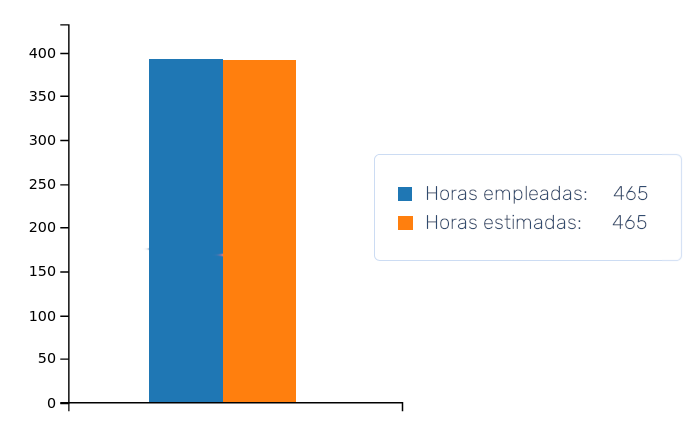
\includegraphics[width=0.6\textwidth]{hours-spent}
	\caption{Horas estimadas frente horas empleadas.}
\end{figure}

En esta planificación, se emplearon dos conceptos ágiles fundamentales:

\vspace{-0.3cm}
\begin{itemize}[\textbullet]
	\item \textbf{Historia de usuario}: se trata de una descripción de una funcionalidad del \emph{software} a implementar.
	\item \textbf{\emph{Epics}}: agrupan historias de usuario que conformen una misma \emph{feature}, o funcionalidad a desarrollar.
\end{itemize}

\vspace{-0.2cm}
En total, se especificaron 99 historias de usuario repartidas entre 8 \emph{epics}\footnote{Para la representación de las historias de usuarios y los \emph{epics} a GitHub se emplearon \emph{Issues} y \emph{Milestones}, respectivamente.}. Estos \emph{epics} fueron, ordenados de manera cronológica:

\vspace{-0.3cm}
\begin{itemize}[\textbullet]
	\item \textbf{Puesta en marcha}: tareas preliminares de organización y puesta en marcha del proyecto (elección de metodologías, herramientas, etc.).

	\item \textbf{Motor de Resumen v0.1}: implementar una primera versión del Motor de Resumen a través de los modelos preentrenados proporcionados por el módulo \texttt{transformers} de Hugging Face \cite{transformers}.

	\item \textbf{Arquitectura Microservicios v0.1}: implementar una primera versión reducida de la Arquitectura de Microservicios, configurando el componente Ingress de Kubernetes \cite{ingress}, y dos microservicios: el Dispatcher y el Pre-procesador de textos.
	
	\item \textbf{Arquitectura Microservicios v0.2}: continuar con la implementación de la arquitectura de microservicios, añadiendo la capacidad de realizar peticiones asíncronas y desarrollando la arquitectura dirigida por eventos. De momento, se sigue trabajando con una versión de la misma, esto es, con el Dispatcher y el  Pre-procesador de textos.

	\item \textbf{Arquitectura Microservicios v0.3}: una vez disponemos de una versión reducida de nuestra arquitectura que funciona correctamente en local, el siguiente paso es desplegarla en Google Kubernetes Engine (GKE) \cite{gke}. Además, se deben implementar los microservicios restantes (Codificador, Motor de Resumen y Post-procesador) y la base de datos para gestionar los resúmenes.
	
	\item \textbf{Cliente v0.1}: desarrollar el cliente (aplicación) que consumirá la API y permitirá al usuario final obtener resúmenes de sus textos. Dicho cliente se implementará con ayuda de Flutter \cite{flutter-es}, por lo que en principio estará disponible en plataformas móvil, \emph{web} y escritorio.
	
	\item \textbf{Arquitectura Microservicios v0.4}: ampliar la especificación de la API para que en las peticiones se puedan detallar todos los parámetros del resumen. Continuar con la mejora del sistema.
	
	\item \textbf{Documentación v0.1}: escribir la Memoria y los Anexos. Generar una primera versión de la documentación de la API REST y del código perteneciente a JIZT.
\end{itemize}

En la \autoref{gantt} se recoge un diagrama Gantt con el objetivo de facilitar la comprensión de la dimensión temporal del proyecto.

\begin{figure}[h]
	\centering
	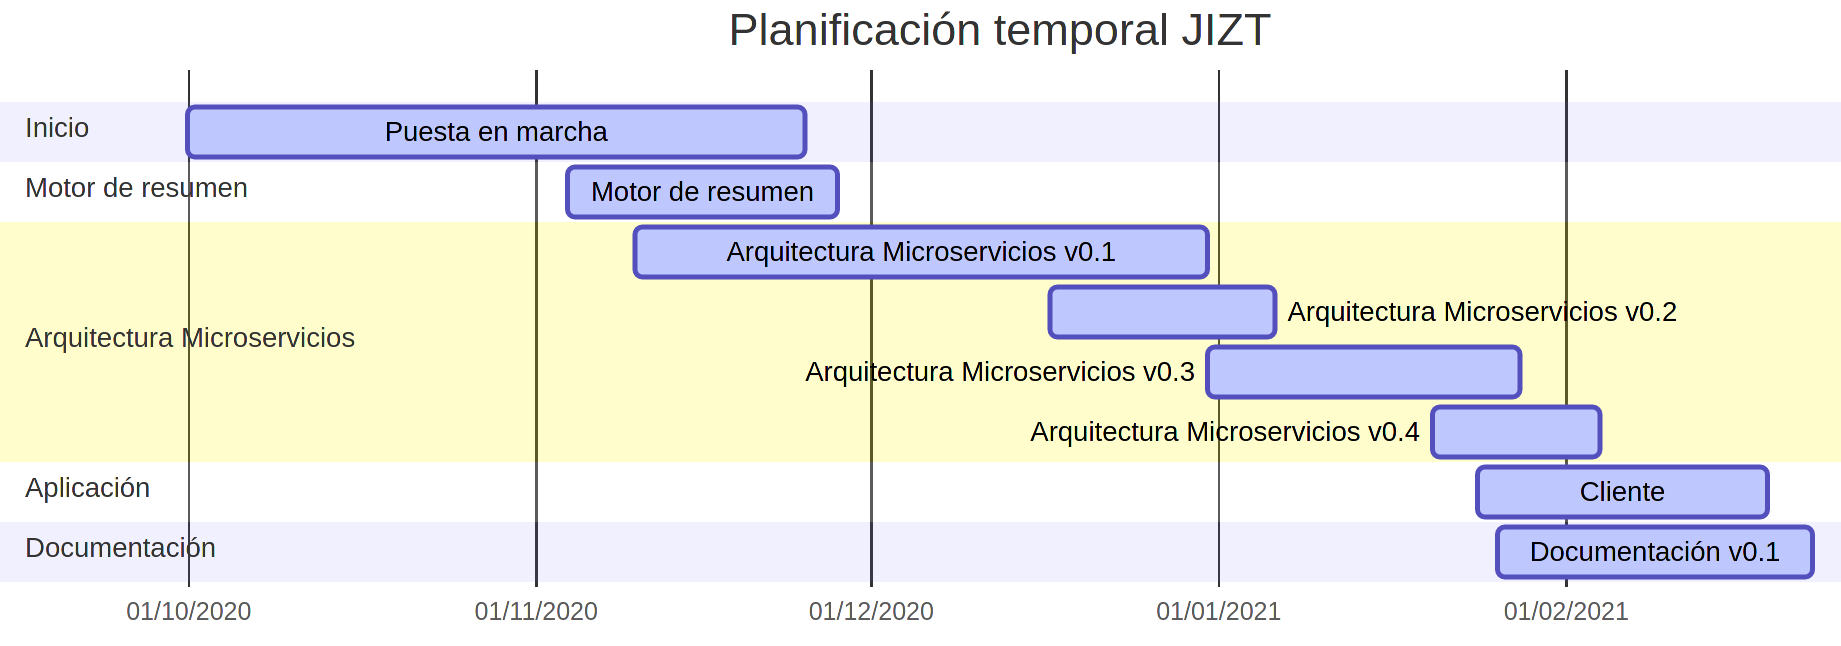
\includegraphics[width=\textwidth]{gantt-epics}
	\vspace{-0.6cm}
	\caption[Diagrama Gantt del proyecto.]{El proyecto comenzó el 1 de octubre de 2021, y finalizó el 16 de febrero de 2021.}
	\label{gantt}
\end{figure}

Dos conceptos importantes dentro de la metodología son \emph{lead time} y \emph{cycle time} \cite{anderson10}. Veamos qué significa cada uno de ellos.

\vspace{-0.3cm}
\begin{itemize}[\textbullet]
	\item \emph{Lead time}: es el período que transcurre entre la aparición de una nueva tarea en el flujo de trabajo y su salida final del sistema. Dicho de otro modo, es el tiempo total que el cliente está esperando la entrega de una parte del producto.
	
	\item \emph{Cycle time}: es la cantidad de tiempo que el equipo realmente empleó en una tarea, es decir, no se cuenta el tiempo que una tarea estuvo <<en espera>>. Por lo tanto, el tiempo del ciclo debe comenzar a medirse cuando la tarea pasa a la columna <<trabajando>>, y no antes.
\end{itemize}

\begin{figure}[h]
	\centering
	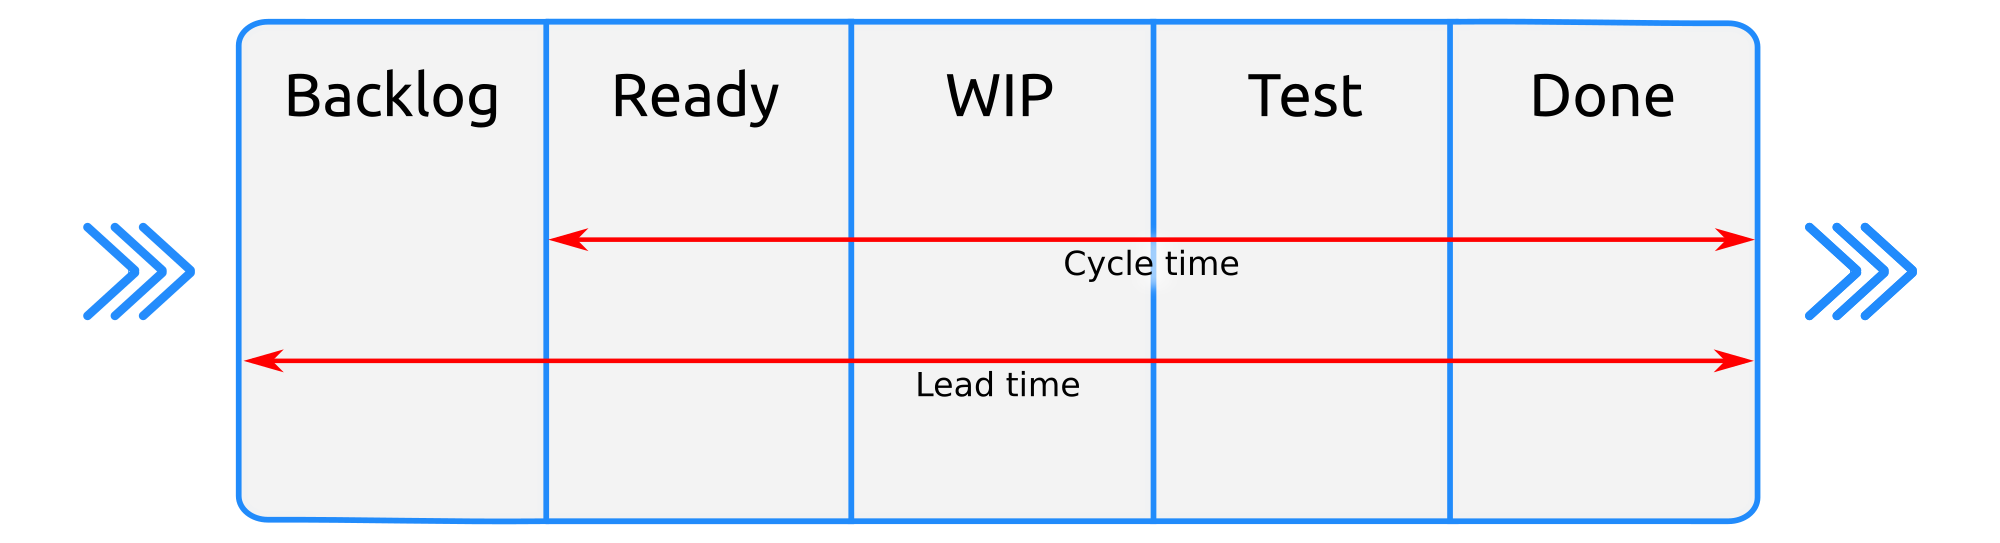
\includegraphics[width=\textwidth]{lead-cycle-time}
	\vspace{-0.6cm}
	\caption[Visualización del \emph{lead} y \emph{cycle time}.]{Explicación gráfica del \emph{lead} y \emph{cycle time} sobre un tablero Kanboard.}
\end{figure}

Esta métrica nos aporta información que nos permite conocer cuánto tiempo tardaremos en entregar una determinada parte del producto. Es importante mantener el \emph{lead} y \emph{cycle time} tan cortos como sea posible, a fin de mantener pocas tareas <<en ejecución>> (WIP), permitiendo mantener un flujo constante de trabajo y aportar valor al cliente de manera frecuente.

\begin{figure}[h]
	\centering
	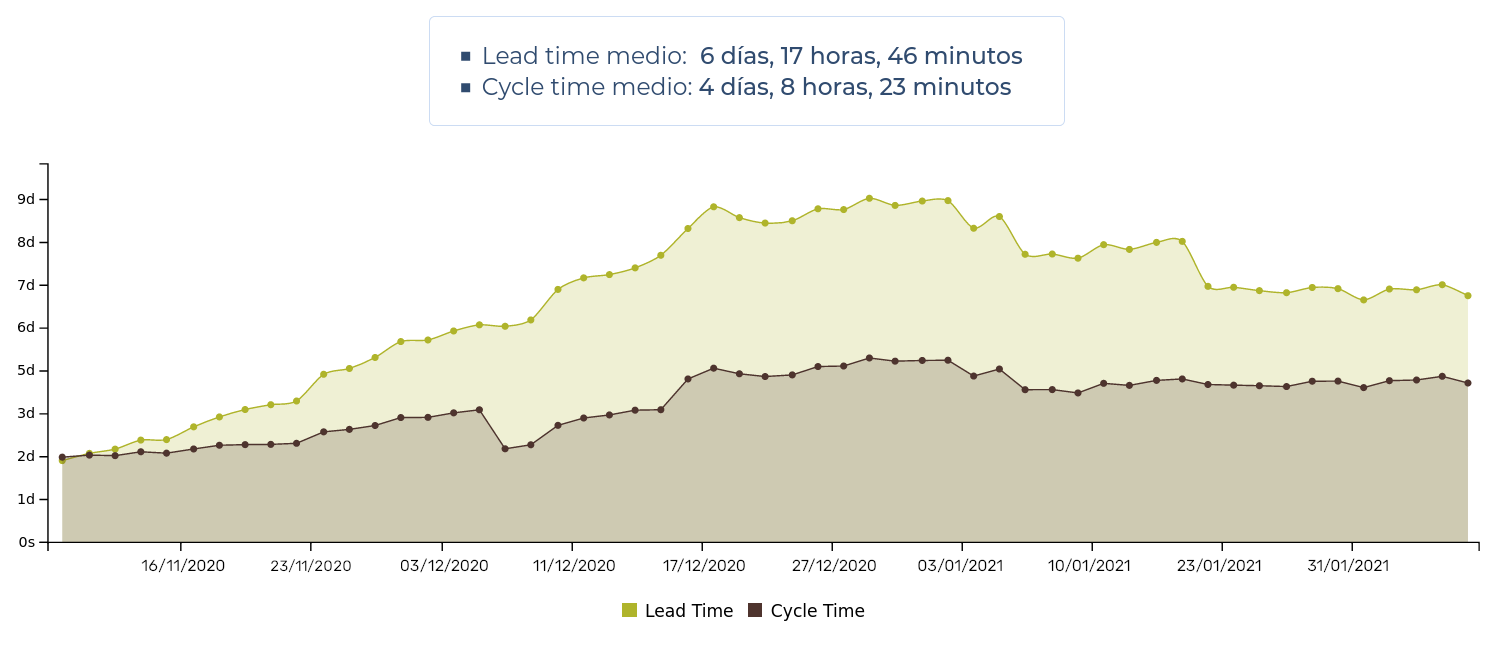
\includegraphics[width=\textwidth]{average-lead-cycle}
	\vspace{-0.7cm}
	\caption{Gráfico de \emph{lead} y \emph{cycle time} medios.}
	\label{average-lead-cycle}
\end{figure}

Como vemos en la \hyperref[average-lead-cycle]{anterior figura}, el \emph{lead time} medio fue de algo menos de 7 días, y el \emph{cycle time} de 4 días y 8 horas. Como es lógico, las primeras tareas se completaron más rápido, pero según la complejidad de las mismas fue incrementándose, también se reflejo en los tiempos. En el punto central del proyecto, se alcanzó una media de \emph{lead time} de 9 días, aunque el \emph{cycle time} se mantuvo por debajo de los 5, lo que indica que existía un mayor número de tareas esperando a ser atendidas.

Otro de los gráficos propios de Kanban que nos puede ofrecer información valiosa es el llamado diagrama de flujo acumulado (CFD, por sus siglas en inglés). Este gráfico muestra el número de tareas que hay en cada columna a lo largo del tiempo.

\begin{figure}[h]
	\centering
	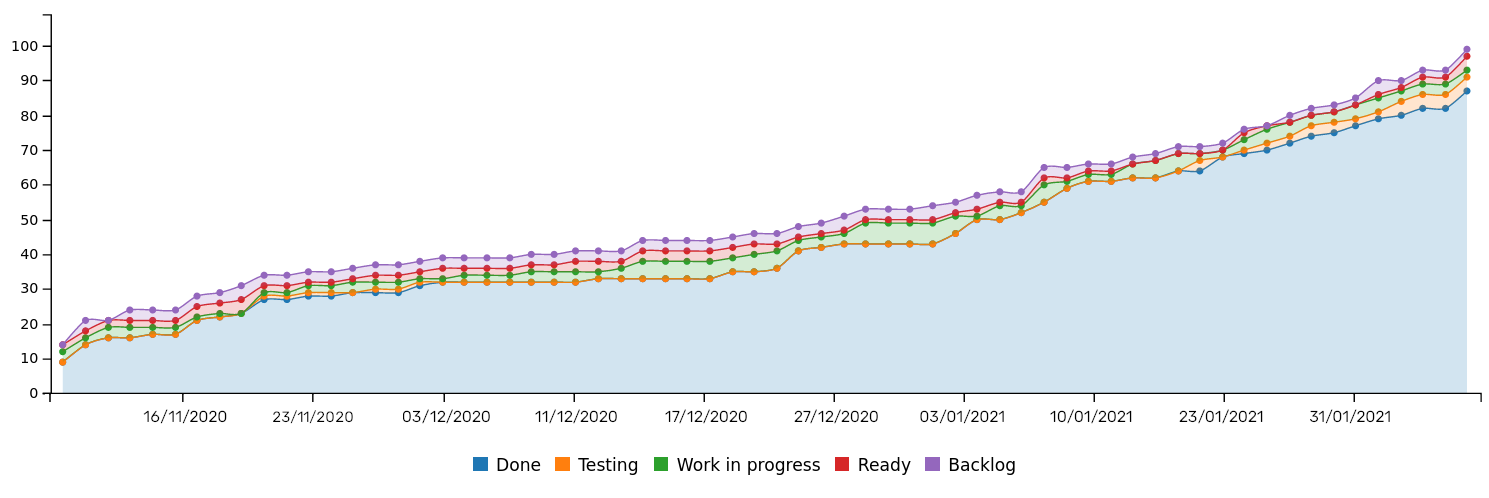
\includegraphics[width=\textwidth]{cfd}
	\vspace{-0.7cm}
	\caption{Diagrama de flujo acumulado desde el comienzo del proyecto.}
	\label{cfd}
\end{figure}

Como podemos ver en el \hyperref[cfd]{anterior diagrama}, el trabajo en las diferentes columnas se distribuyó de forma correcta, no apareciendo grandes diferencias entre ellas. En este gráfico, también podemos apreciar que en la parte central del proyecto, las tareas en <<\emph{Work in progress}>> fueron algo mayores que en el resto de columnas, lo cual es comprensible.

El diagrama de flujo acumulado obtenido muestra también que el ritmo de trabajo fue constante, incrementándose ligeramente hacia el final del proyecto.

Podemos visualizar también la distribución de las tareas en función de su tipo:

\begin{figure}[h]
	\centering
	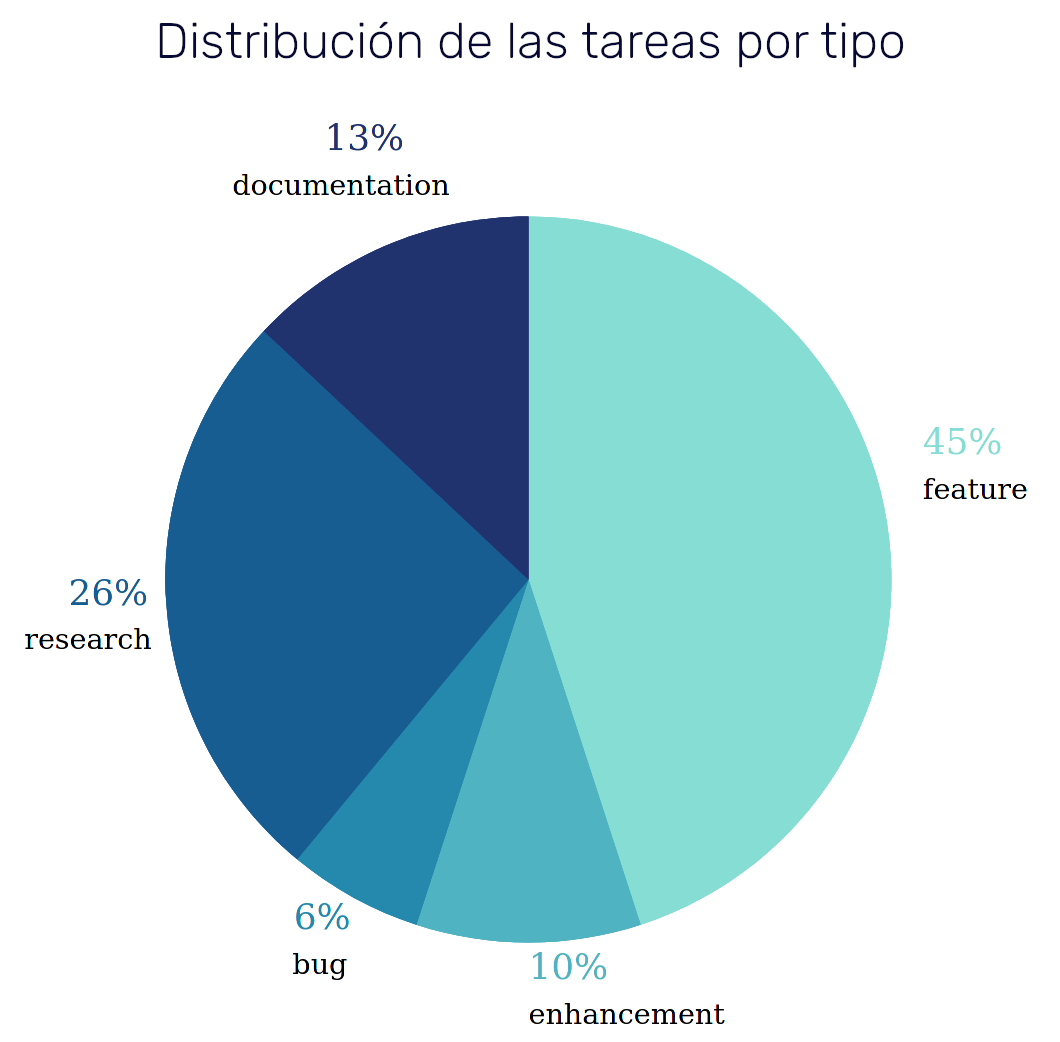
\includegraphics[width=0.7\textwidth]{distribucion-tareas}
	\caption{Distribución de las tareas según su tipo.}
\end{figure}

Como es lógico, la mayor parte de las tareas se dedicaron a ofrecer nuevas funcionalidades (\emph{feature}), aunque gran número de ellas se dedicaron al aprendizaje y búsqueda de información (\emph{research}), lo cual también parece ajustarse a la realidad, puesto que como ya hemos mencionado, muchas de las herramientas y técnicas que hemos utilizado eran nuevas para nosotros. 

Para finalizar esta sección, cabe mencionar que en el \href{https://github.com/dmlls/jizt/milestones}{repositorio del proyecto}, y en su \href{https://board.jizt.it/public/board/c08ea3322e2876652a0581e79d6430e2dc0c27720d8a06d7853e84c3cd2b}{tablero Kanban}, se puede encontrar información más detallada de cada historia de usuario y \emph{epic}.

\newpage

\section{Estudio de viabilidad}

\subsection{Viabilidad económica}

Uno de los puntos cruciales a la hora de estudiar la viabilidad de un proyecto, y que en muchos casos determina el éxito o el fracaso del mismo, es la viabilidad económica.

En esta sección analizamos los costes y beneficios de JIZT.


\subsubsection{Costes del proyecto}

En nuestro caso, dividiremos los costes del proyecto n costes fijos, directos e indirectos.

\vspace{0.4cm}
\noindent
\textbf{\emph{Costes fijos}}

Los costes fijos son aquellos costes invariables que debemos abonar, independientemente del desarrollo del proyecto \cite{perez18}.

\begin{table}[h!]
	\centering
	\begin{tabular}{>{\raggedright}b{0.6\linewidth}>{\raggedleft\arraybackslash}b{0.2\linewidth}}
		\toprule
		\textbf{{\scriptsize CONCEPTO}}  & \textbf{{\scriptsize IMPORTE}} \\
		\midrule
		\small{\; Servicio de Internet} & \small{200,00 €} \\
		\midrule
		\small{\; Servicio de Luz$^1$} & \small{225,00 €} \\
		\midrule
		\small{\; Materiales de oficina} & \small{5,00 €} \\
		\midrule
		\small{\; Salarios$^2$} & \small{9911,88 €} \\
		\scriptsize{\qquad Salario mensual neto} & \scriptsize{1000,00 €} \\
		\scriptsize{\qquad Retenciones1 por IRPF (24 \%)$^3$} & \scriptsize{528,63 €} \\
		\scriptsize{\qquad Cuotas a la Seg. Social (30,6 \%)$^4$} & \scriptsize{674,01 €} \\
		\scriptsize{\qquad Salario mensual bruto} & \scriptsize{2202,64 €} \\
		\bottomrule
		\textbf{{\scriptsize TOTAL}}  & \textbf{\small 10341,88 €} \\
		\bottomrule
		\multicolumn{2}{l}{\scriptsize{$^1$ Costes calculados para 4,5 meses, con tarifa de mercado libre y potencia}} \\
		\multicolumn{2}{l}{\hspace{0.11cm} \scriptsize{contratada de 3,3 kW (precio mensual medio de 50 €).}} \\
		\multicolumn{2}{l}{\scriptsize{$^2$ Costes calculados para 4,5 meses.}} \\
		\multicolumn{2}{l}{\scriptsize{$^3$ Según la tabla de retenciones por IRPF aplicable al ejercicio 2021 \cite{irpf21}}} \\
		\multicolumn{2}{l}{\scriptsize{$^4$ Porcentaje para autónomos según la Ley 11/2020, de 30 de diciembre, de}} \\
		\multicolumn{2}{l}{\hspace{0.11cm} \scriptsize{Presupuestos Generales del Estado para el año 2021 \cite{boe341}.}} \\
		\bottomrule
	\end{tabular}
	\caption{Desglose de costes fijos del proyecto.}
\end{table}

\newpage

\noindent
\textbf{\emph{Costes directos}}

Los costes directos son aquellos costes derivados directamente del desarrollo del proyecto.

\begin{table}[h!]
	\centering
	\begin{tabular}{>{\raggedright}m{0.58\linewidth}>{\raggedleft}m{0.16\linewidth}>{\raggedleft\arraybackslash}m{0.15\linewidth}}
		\toprule
		\textbf{{\scriptsize CONCEPTO}}  & \textbf{{\scriptsize IMPORTE}} & \textbf{{\scriptsize IMPORTE AMORTIZ.}} \\
		\midrule
		\small{\; Costes de \emph{hardware}$^1$} & \small{2509,58 €} & \small{79,49 €} \\
		\scriptsize{\qquad Ordenador personal} & \scriptsize{845,00 €} & \scriptsize{63,37 €} \\
		\scriptsize{\qquad \emph{Smartphone} Android} & \scriptsize{215,00 €} & \scriptsize{16,12 €} \\
		\scriptsize{\qquad Servicio GKE$^2$ de Google Cloud} & \scriptsize{1449,58 €} & - \\
		\midrule
		\small{\; Costes de \emph{software}$^3$} & \small{89,95 €} & \small{16,86 €} \\
		\scriptsize{\qquad Adobe Illustrator} & \scriptsize{89,95 €} &  \scriptsize{16,86 €} \\

	
		\bottomrule
		\textbf{{\scriptsize TOTAL}}  & \textbf{\small 2599,53 €} & \textbf{\small 96,35 €} \\
		\bottomrule
		\multicolumn{3}{l}{\scriptsize{$^1$ Se han calculado con una amortización de 5 años, habiendo sido utilizado 4,5 meses.}} \\
		\multicolumn{3}{l}{\scriptsize{$^2$ Google Kubernetes Engine \cite{gke}.}} \\
		\multicolumn{3}{l}{\scriptsize{$^1$ Se han calculado con una amortización de 2 años, habiendo sido utilizado 4,5 meses.}} \\
		\bottomrule
	\end{tabular}
	\caption{Desglose de costes directos del proyecto.}
\end{table}

\noindent
\textbf{\emph{Costes indirectos}}

Los costes indirectos son aquellos que no dependen directamente del desarrollo del proyecto.

\begin{table}[h!]
	\centering
	\begin{tabular}{>{\raggedright}b{0.6\linewidth}>{\raggedleft\arraybackslash}b{0.2\linewidth}}
		\toprule
		\textbf{{\scriptsize CONCEPTO}}  & \textbf{{\scriptsize IMPORTE}} \\
		\midrule
		\small{\; Dominio \href{https://www.jizt.it}{jizt.it}} & \small{4,81 €} \\
		\small{\; Cuenta de Google Play} & \small{20,76 €} \\
		\small{\; Impresión de la Memoria y el cartel del TFG} & \small{40,00 €} \\
		\bottomrule
		\textbf{{\scriptsize TOTAL}}  & \textbf{\small 65,57 €} \\
		\bottomrule
	\end{tabular}
	\caption{Desglose de costes indirectos del proyecto.}
\end{table}

\noindent
\textbf{\emph{Costes totales del proyecto}}

Considerando las tres categorías de costes recogidas anteriormente, la suma de los costes totales del proyecto asciende a \textbf{13006,10 €}.

\newpage

\subsubsection{Beneficios}

La API REST de JIZT se ofrece en tres planes de suscripción diferentes.

\vspace{-0.3cm}
\begin{itemize}[\textbullet]
	\item \textbf{\emph{Gratuito}}: este plan se ajusta a las necesidades de cualquier usuario regular que no vaya a realizar un uso exhaustivo del servicio. Se permiten 5.000 peticiones a la API REST, pudiendo hacerse hasta 5 peticiones por minuto. No incluye soporte técnico.
	
	\item \textbf{Estándar}: para aquellas empresas o particulares que van a realizar un uso más intensivo del servicio. Se incluyen 15.000 peticiones a la API REST, pudiendo hacerse hasta 15 peticiones por minuto. Incluye soporte técnico y de integración. El precio es de 166 €/mes.
	
	\item \textbf{Personalizado}: para aquellos usuarios cuyas necesidades no encajen en ninguno de los anteriores precios. El precio se establecerá en función de los requerimientos concretos del usuario.
\end{itemize}

En cuanto a la aplicación, es totalmente gratuita y no contiene publicidad.

\newpage
\subsection{Análisis DAFO}

Tras llevar a cabo un pequeño análisis de mercado, hemos identificado que las principales debilidades, amenazas, fortalezas y oportunidades de nuestro proyecto son las siguientes:

\begin{figure}[h]
	\centering
	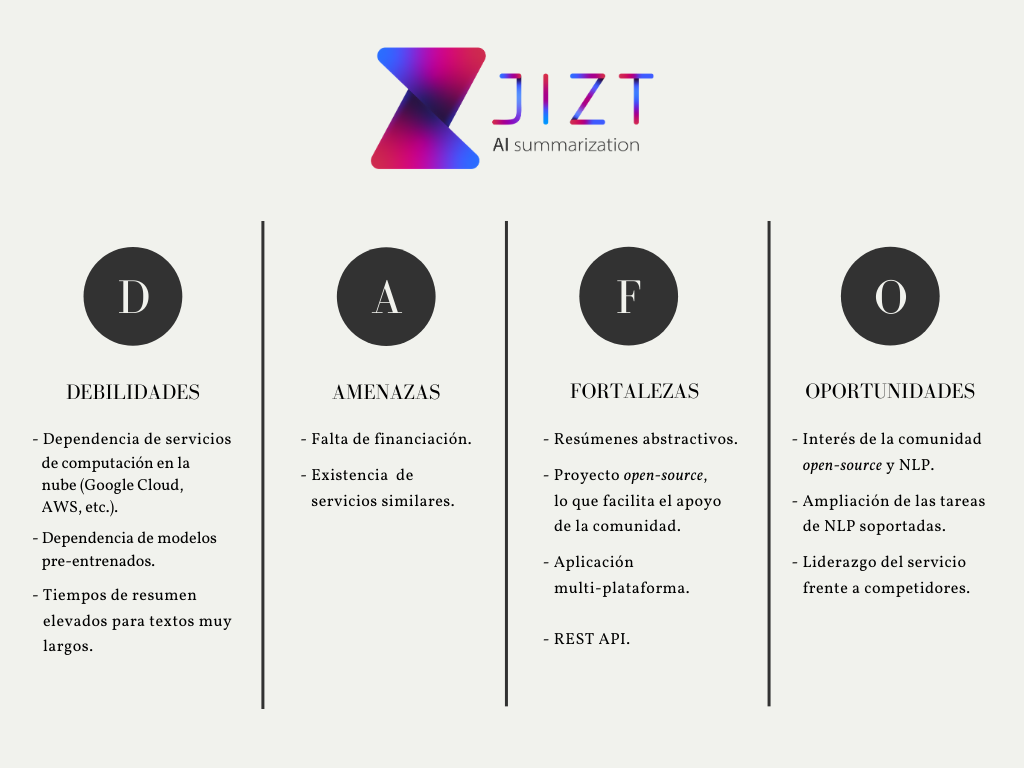
\includegraphics[width=1\textwidth]{dafo}
	\vspace{-0.5cm}
	\caption{Análisis DAFO de JIZT.}
\end{figure}

\subsection{Viabilidad legal}

\subsubsection{Licencia del código fuente del proyecto}

Desde un primer momento nuestra intencción era licenciar el proyecto bajo una licencia de \emph{Software} Libre. Dentro de este entorno, se han considerado las tres licencias más extendidas: Apache-2.0, MIT, y GPLv3.

Tras una lectura exhaustiva de las cláusulas de cada una de ellas, así como de opiniones en \emph{blogs}, charlas, foros, etc., y tras una profunda reflexión, considerando especialmente la licencia MIT y la GPLv3, hemos tomado la decisión de que nuestro software estará licenciado bajo \textbf{GNU GPLv3} \cite{gplv3}, cuyos puntos principales se recogen en la \autoref{gnu-gpl3}.

\begin{figure}[h]
	\centering
	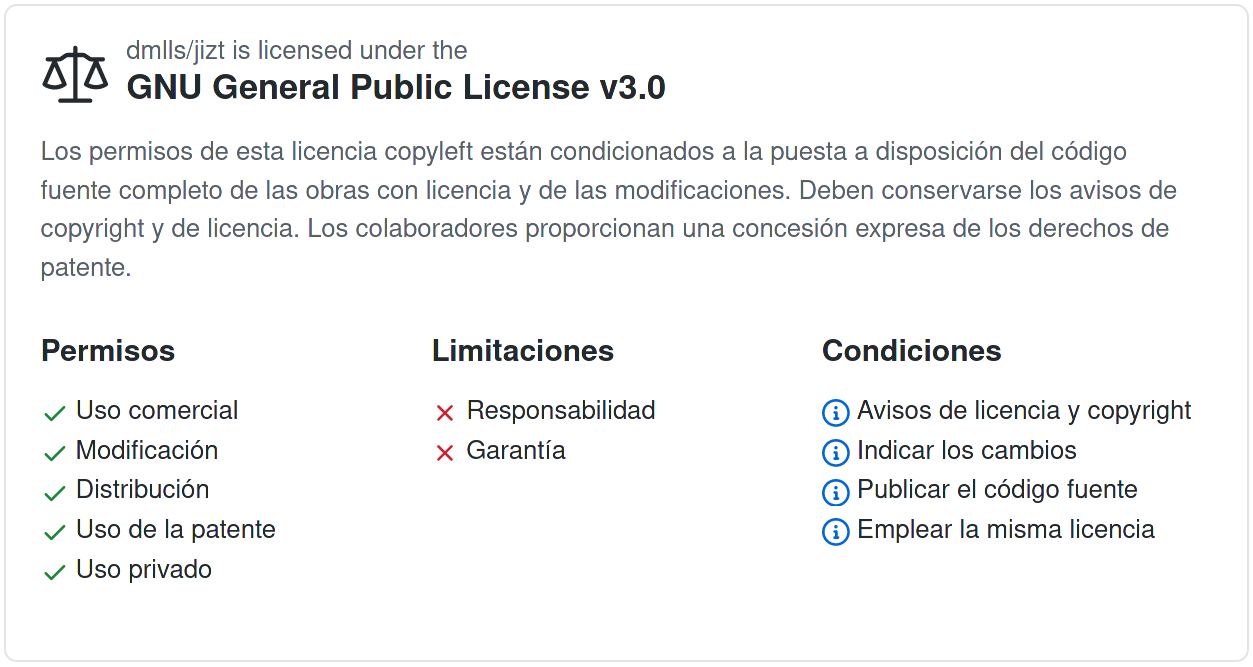
\includegraphics[width=1\textwidth]{gnu-gpl3}
	\vspace{-0.5cm}
	\caption[Resumen de la licencia GNU GPLv3]{Resumen de la licencia GNU GPLv3. Imagen extraída y traducida de \href{https://github.com/dmlls/jizt/blob/main/LICENSE}{https://github.com/dmlls/jizt/blob/main/LICENSE}.}
	\label{gnu-gpl3}
\end{figure}

Las principales razones de nuestra elección son:

\vspace{-0.3cm}
\begin{itemize}[\textbullet]
	\item Pese a que la licencia MIT pueda parecer más permisiva en un primer lugar, ya que no obliga a que el código fuente se mantenga abierto en un futuro, creemos que a largo plazo esta <<permisividad>>, paradójicamente, puede resultar en una limitación de sí misma. Esto es, el hecho de que ese supuesto \emph{software} <<libre>> se pueda volver \emph{software} <<cerrado>>, lo excluye en primer lugar de esa definición de <<libre>>, en nuestra opinión.

	\item Este proyecto no podría existir sin las contribuciones de \emph{software} libre anteriores. Por ello, queremos asegurar que este proyecto siempre se mantenga abierto para poder ayudar a otros y retroalimentarse con los aportes de la comunidad.
	
	\item El simple hecho de elegir una licencia, conlleva un sinnúmero de implicaciones morales, económicas, sociales, etc., pero es algo necesario, ya que el \emph{software} sin licencia explícita se toma por defecto como \emph{copyright}.
\end{itemize}

\newpage

\noindent
\textbf{Listado de dependencias}

Todas las dependencias del proyecto se encuentran licenciadas bajo licencias compatibles con GNU GPLv3.

A continuación, se recoge una lista detallada de las mismas:

\begin{table}[h!]
	\centering
	\begin{tabular}{>{\raggedright}b{0.25\linewidth}>{\centering}b{0.15\linewidth}>{\raggedright}b{0.3\linewidth}>{\raggedleft\arraybackslash}b{0.15\linewidth}}
		\toprule
		\textbf{Dependencia} & \textbf{Versión} & \textbf{Descripción} & \textbf{Licencia} \\
		\midrule
		\small{\; API REST} & & & \\
		\small{\qquad \texttt{NLTK}} & \small{3.5} & \scriptsize{Utilidades de NLP.} & \small{Apache v2.0} \\
		\small{\qquad \texttt{transformers}} & \small{4.1.1} & \scriptsize{Modelos pre-entrenados.} & \small{Apache v2.0} \\
		\small{\qquad \texttt{truecase}} & \small{0.0.12} & \scriptsize{\emph{Truecaser}.} & \small{Apache v2.0} \\
		\small{\qquad \texttt{confluent}-\\ \qquad \texttt{kafka}} & \small{1.5.0} \\ & \scriptsize{Cliente de Kafka para} \\ \scriptsize{Python.} & \small{Apache v2.0} \newline \\
		\small{\qquad \texttt{strimzi}-\\ \qquad \texttt{operator}} & \small{0.21.0} \\ & \scriptsize{Kafka en Kubernetes.} \\ \scriptsize{} & \small{Apache v2.0} \newline \\
		\small{\qquad \texttt{postgres}-\\ \qquad \texttt{operator}} & \small{0.21.0} \\ & \scriptsize{PostgreSQL en Kubernetes.} \\ \scriptsize{} & \small{Apache v2.0} \newline \\
		\small{\qquad \texttt{blingfire}} & \small{0.1.3} & \scriptsize{Utilidades de NLP.} & \small{MIT} \\
		\small{\qquad \texttt{marshmallow} \\ \texttt{}} & \small{3.10.0} \\ & \scriptsize{Serialización y de-} \\ \scriptsize{serialización.} & \small{\hspace{1.1cm} MIT} \newline \\
		
		\midrule
		
		\small{\; Aplicación} & & & \\
		\bottomrule
	\end{tabular}
	\caption{Listado de dependencias.}
\end{table}1

\subsubsection{Licencia de la documentación del proyecto}

La totalidad de la documentación de JIZT se distribuye bajo licencia GNU Free Documentation License (GFDL) \cite{gfdl}.

Esta licencia es una adaptación al contexto de la documentación de la GNU General Public License (GPL), la cual está pensada para licenciar código fuente.

La GFDL da permiso a los lectores de copiar, redistribuir y modificar (excepto las <<secciones invariables>>) una obra y exige que todas las copias y derivados estén disponibles bajo la misma licencia. Las copias también pueden venderse comercialmente, pero, si se producen en grandes cantidades (más de 100), el documento original o el código fuente deben ponerse a disposición del destinatario de la obra \cite{gfdl}. 

\apendice{Especificación de Requisitos}

\section{Introducción}

En este apéndice se recoge una descripción del sistema \emph{software} a desarrollar. Más concretamente, se presentan aspectos como el propósito, alcance y objetivos generales del mismo, así como los requisitos específicos que el sistema debe implementar.

La forma en la que hemos organizado la Especificación está basada parcialmente en las recomendaciones del estándar IEEE 830-1998, considerado como la principal referencia para la aplicación de buenas prácticas en la escritura del Documento de Especificación de Requistios (SRS).

\subsection{Propósito}

El propósito de la presente Especificación de Requisitos tiene como objetivo ofrecer una descripción detallada del sistema \emph{software} desarrollado.

Este documento está orientado principalmente al equipo de desarrollo del proyecto, pero queda también a libre disposición de cualquier persona que pudiera estar interesada.

\subsection{Alcance}

El sistema \emph{software} a desarrollar recibirá el nombre de JIZT. El objetivo y funcionalidad principal de JIZT será la generación de resúmenes abstractivos en la nube. Dicho sistema estará orientado tanto a usuarios con conocimientos de informática básicos, así como usuarios con experiencia en el campo.

Para los primeros, es decir, usuarios con conocimientos básicos, se ofrecerá una aplicación multiplataforma desarrollada con la usabilidad en mente.

Para aquellos usuarios más avanzados, además de la aplicación, se proporcionará una API REST, permitiéndoles realizar peticiones directamente, e incluso desarrollar sus propias aplicaciones que consuman dicha API.

Se pondrá especial atención en el desarrollo de una documentación completa, accesible y de fácil comprensión. Esta documentación recogerá tanto los aspectos técnicos de la aplicación y la API REST, así como manuales de uso para el usuario y para el desarrollador.

\subsection{Definiciones, siglas, y abreviaciones}

A continuación se recogen las definiciones, siglas y abreviaciones más relevantes para el proyecto:

\vspace{-0.3cm}
\begin{itemize} [\textbullet]
	\item \textbf{NLP}: Procesamiento de Lenguaje Natural (\emph{Natural Language Processing}).
	\vspace{-0.1cm}
	\item \textbf{Resumen extractivo}: aquel resumen generado a partir de la \emph{extracción} de las frases del texto consideradas más relevantes. Es decir, este tipo de resúmenes contienen únicamente frases tomadas literalmente del texto original.
	\vspace{-0.1cm}
	\item \textbf{Resumen abstractivo}: aquel resumen que incluye palabras o expresiones que no aparecen en el texto original.
	\vspace{-0.1cm}
	\item \textbf{API REST}: servicio \emph{web} que proporciona una serie de \emph{endpoints} para llevar a cabo operaciones HTTP (métodos), que proporcionan acceso para crear, recuperar, actualizar o eliminar los recursos del servicio.
	\vspace{-0.1cm}
	\item \textbf{\emph{Endpoint}}: punto de entrada en un canal de comunicación cuando dos sistemas interactúan. En una API REST los \emph{endpoints} son generalmente URLs.
	\vspace{-0.1cm}
	\item \textbf{HTTP}: \emph{Hypertext Transfer Protocol}, protocolo para sistemas de información distribuidos, colaborativos e hipermedia. Este protocolo es la base de la comunicación de datos para la World Wide Web (WWW).
	\vspace{-0.1cm}
	\item \textbf{URL}: \emph{Uniform Resource Locator}, referencia a un recurso web que especifica su ubicación en una red informática y un mecanismo para recuperarlo.
	\vspace{-0.1cm}
	\item \textbf{\emph{Frontend}}: la infraestructura \emph{frontend} incluye todos aquellos elementos del sistema con los que el usuario final interactúa.
	\vspace{-0.1cm}
	\item \textbf{\emph{Backend}}:parte de la infraestructura que contiene el conjunto de servidores, bases de datos, APIs y los sistemas operativos que alimentan el \emph{frontend} de una aplicación.
\end{itemize}

\section{Descripción global}

\subsection{Objetivos generales}

Los principales objetivos del sistema \emph{software} a desarrollar son los siguientes:

\vspace{-0.3cm}
\begin{itemize} [\textbullet]
	\item Implementar un servicio de generación de resúmenes abstractivos en la nube, empleando modelos pre-entrenados del estado del arte.
	\vspace{-0.1cm}
	\item Implementar el \emph{backend} que haga posible esta generación de resúmenes, así como una API REST para exponer el \emph{backend}.
	\vspace{-0.1cm}
	\item Diseñar la arquitectura del \emph{backend} con aspectos como la flexibilidad, la escalabilidad y la alta disponibilidad como pilares fundamentales.
	\vspace{-0.1cm}
	\item Implementar un \emph{frontend} (aplicación multiplataforma) que consuma la REST API y dé la posibilidad de generar resúmenes a cualquier usuario.
	\vspace{-0.1cm}
	\item Implementar una interfaz (tanto en el \emph{backend} como en el \emph{fontend}) que permita a los usuarios especificar los parámetros con los que el resumen será generado, como por ejemplo, su longitud relativa al texto original.
	
\end{itemize}


\subsection{Características del usuario}

Los usuarios potenciales de JIZT se pueden dividir en dos categorías fundamentales:

\vspace{-0.3cm}
\begin{itemize} [\textbullet]
	\item Estudiantes de edades comprendidas entre los 15 y 25 años. El uso principal que harán del producto será el resumen de textos académicos.
	\item Personas de edades comprendidas entre los 25 y 50 años, cuyo principal uso será el resumen de noticias y artículos periodísticos.
\end{itemize}

En cuanto al sexo, el uso por parte tanto de hombres como mujeres será aproximadamente equivalente.

Un tercer tipo de usuario, no incluido anteriormente, serían partidos interesados en el uso del producto (empresas, particulares, etc.), que fueran a hacer un uso extensivo y exhaustivo del mismo. Este tipo de usuario requiere unas prestaciones más exigentes, pudiendo llegar a solicitar el despliegue de JIZT en sus propias dependencias.

Es por ello que el producto desarrollado deberá ser lo más independiente del entorno en el que se despliegue como sea posible.


\section{Catalogo de requisitos}

A continuación se detallan los requisitos funcionales y no funcionales del producto a desarrollar. Estos requisitos son globales al proyecto y, por tanto, involucran tanto al \emph{backend} como a la aplicación a desarrollar.

\subsection{Requisitos funcionales}

\begin{itemize}[\textbullet]
	\item \textbf{RF-1 Solicitar resumen}: la API REST debe proporcionar un \emph{endpoint} para que el usuario pueda solicitar un resumen de un texto.
	\begin{itemize}[◦]
		\item \textbf{RF-1.1 Elegir modelo de generación de resumen}: el usuario deberá ser capaz de especificar el modelo de generar su resumen\footnote{\, Este requisito solo se ha implementado en el \emph{backend}. En la aplicación decidimos no incluirlo dado que por el momento solo hacemos uso de un modelo.}.
		\item \textbf{RF-1.2 Especificar longitud relativa del resumen}: el usuario deberá ser capaz de especificar la longitud del resumen generado, de manera relativa al texto original.
		\item \textbf{RF-1.3 Especificar parámetros del resumen}: el usuario deberá ser capaz de especificar los parámetros concretos con los que se generará su resumen\footnote{\, Este requisito solo se ha implementado en el \emph{backend}. En la aplicación se añadirá en futuras iteraciones, al considerarse no prioritario, dado que se trata de opciones avanzadas.}.
	\end{itemize}
	\item \textbf{RF-2 Historial de resúmenes}: el usuario podrá acceder a los resúmenes que ha generado recientemente.
	\item \textbf{RF-3 Compartir resumen}: se le brindará al usuario la opción de compartir el resumen generado a través de otra aplicación a su elección.
	\item \textbf{RF-4 Copiar resumen}: se le brindará al usuario la opción de copiar el resumen generado.
	\item \textbf{RF-5 Borrar resumen}: el usuario deberá ser capaz de borrar permanentemente un resumen previamente generado.
	\item \textbf{RF-6 Pegar desde el portapapeles}: la aplicación ofrecerá una opción para que el usuario pueda pegar el texto a resumir desde el portapapeles de forma sencilla.
	\item \textbf{RF-7 Mostrar metadatos}: el sistema brindará al usuario los metadatos relativos al resumen generado, como la hora a la que fue creado.
	\item \textbf{RF-8 Pre-procesado del texto}: el sistema será capaz de recibir texto con errores de formateo (exceso de espacios, saltos de carro situados en mitad de una frase, etc.), así como caracteres <<extraños>>. Independientemente de lo anterior, el resumen generado aparecerá correctamente formateado y sin los mencionados caracteres.
	\item \textbf{RF-9 Textos arbitrariamente largos}: el sistema será capaz de producir resúmenes de cualquier texto, independientemente de la longitud de los mismos. No se espera, no obstante, que el tiempo de resumen de textos extremadamente largos esté por debajo del orden del minuto.
\end{itemize}

\subsection{Requisitos no funcionales}

\begin{itemize}[\textbullet]
	\item \textbf{RNF-1 Escalabilidad}: la arquitectura del sistema deberá permitir el escalado del mismo de forma rápida y sencilla.
	\begin{itemize}[◦]
		\item \textbf{RNF-1.1 Autoescalado}: el sistema podrá escalarse de manera automática en momentos en los que la carga de trabajo así lo requiera. Del mismo modo, cuando dicha carga remita, deberá disminuir su escala, a fin de consumir los mínimos recursos posibles.
	\end{itemize}
	\item \textbf{RNF-2 Alta disponibilidad}: el sistema deberá garantizar el acceso al mismo por parte de los usuarios en el 99,99 \% de los casos.
	\begin{itemize}[◦]
		\item \textbf{RNF-2.1 Tolerancia frente a fallos}: el sistema deberá ser capaz de recuperarse de forma automática de posibles errores o problemas de funcionamiento de cualquiera de sus componentes en un tiempo menor a los 2 minutos.
	\end{itemize}
	\item \textbf{RNF-3 Eficiencia}: el sistema deberá ser capaz de generar un elevado número de resúmenes provenientes de diferentes usuarios de forma simultánea, sin que el tiempo medio de resumen se vea afectado.
	\item \textbf{RNF-4 Seguridad lógica y de datos}: se debe garantizar la correcta protección de todos los datos manejados por el sistema.
	\item \textbf{RNF-5 Privacidad}: se debe asegurar la protección de los datos de carácter personal.
	\begin{itemize}[◦]
		\item \textbf{RNF-5.1 Anonimidad}: en ningún caso se recopilará información de los usuarios que permita determinar la identidad de los mismos. No obstante, el sistema no es responsable de garantizar que los textos introducidos no contienen información de carácter personal.
	\end{itemize}
	\item \textbf{RNF-6 Usabilidad}: el tiempo medio de aprendizaje de la aplicación por parte de los usuarios deberá ser inferior a los 5 minutos. Además, el sistema contará con documentación en línea detallada del producto.
	\item \textbf{RNF-7 Multiplataforma}: se distribuirán los binarios de la aplicación necesarios para su ejecución en móvil (Android e iOS), \emph{web} (Google Chrome, Mozilla Firefox, Safari y Microsoft Edge), y escritorio (Linux, Apple y Windows).
	\item \textbf{RNF-8 Tamaño reducido}: el peso de la aplicación no debe superar los 30 MB.
\end{itemize}

\newpage

\section{Especificación de requisitos}

En esta sección, nos centramos en la definición de los casos de uso de nuestro producto.

Dado que el usuario interactuará únicamente con la aplicación (\emph{frontend}), el \emph{backend} no se considera en este caso, aunque sigue siendo vital para que los casos de uso de la aplicación se puedan completar con éxito.

\subsection{Diagrama de casos de uso}



\begin{figure}[h!]
	\centering
	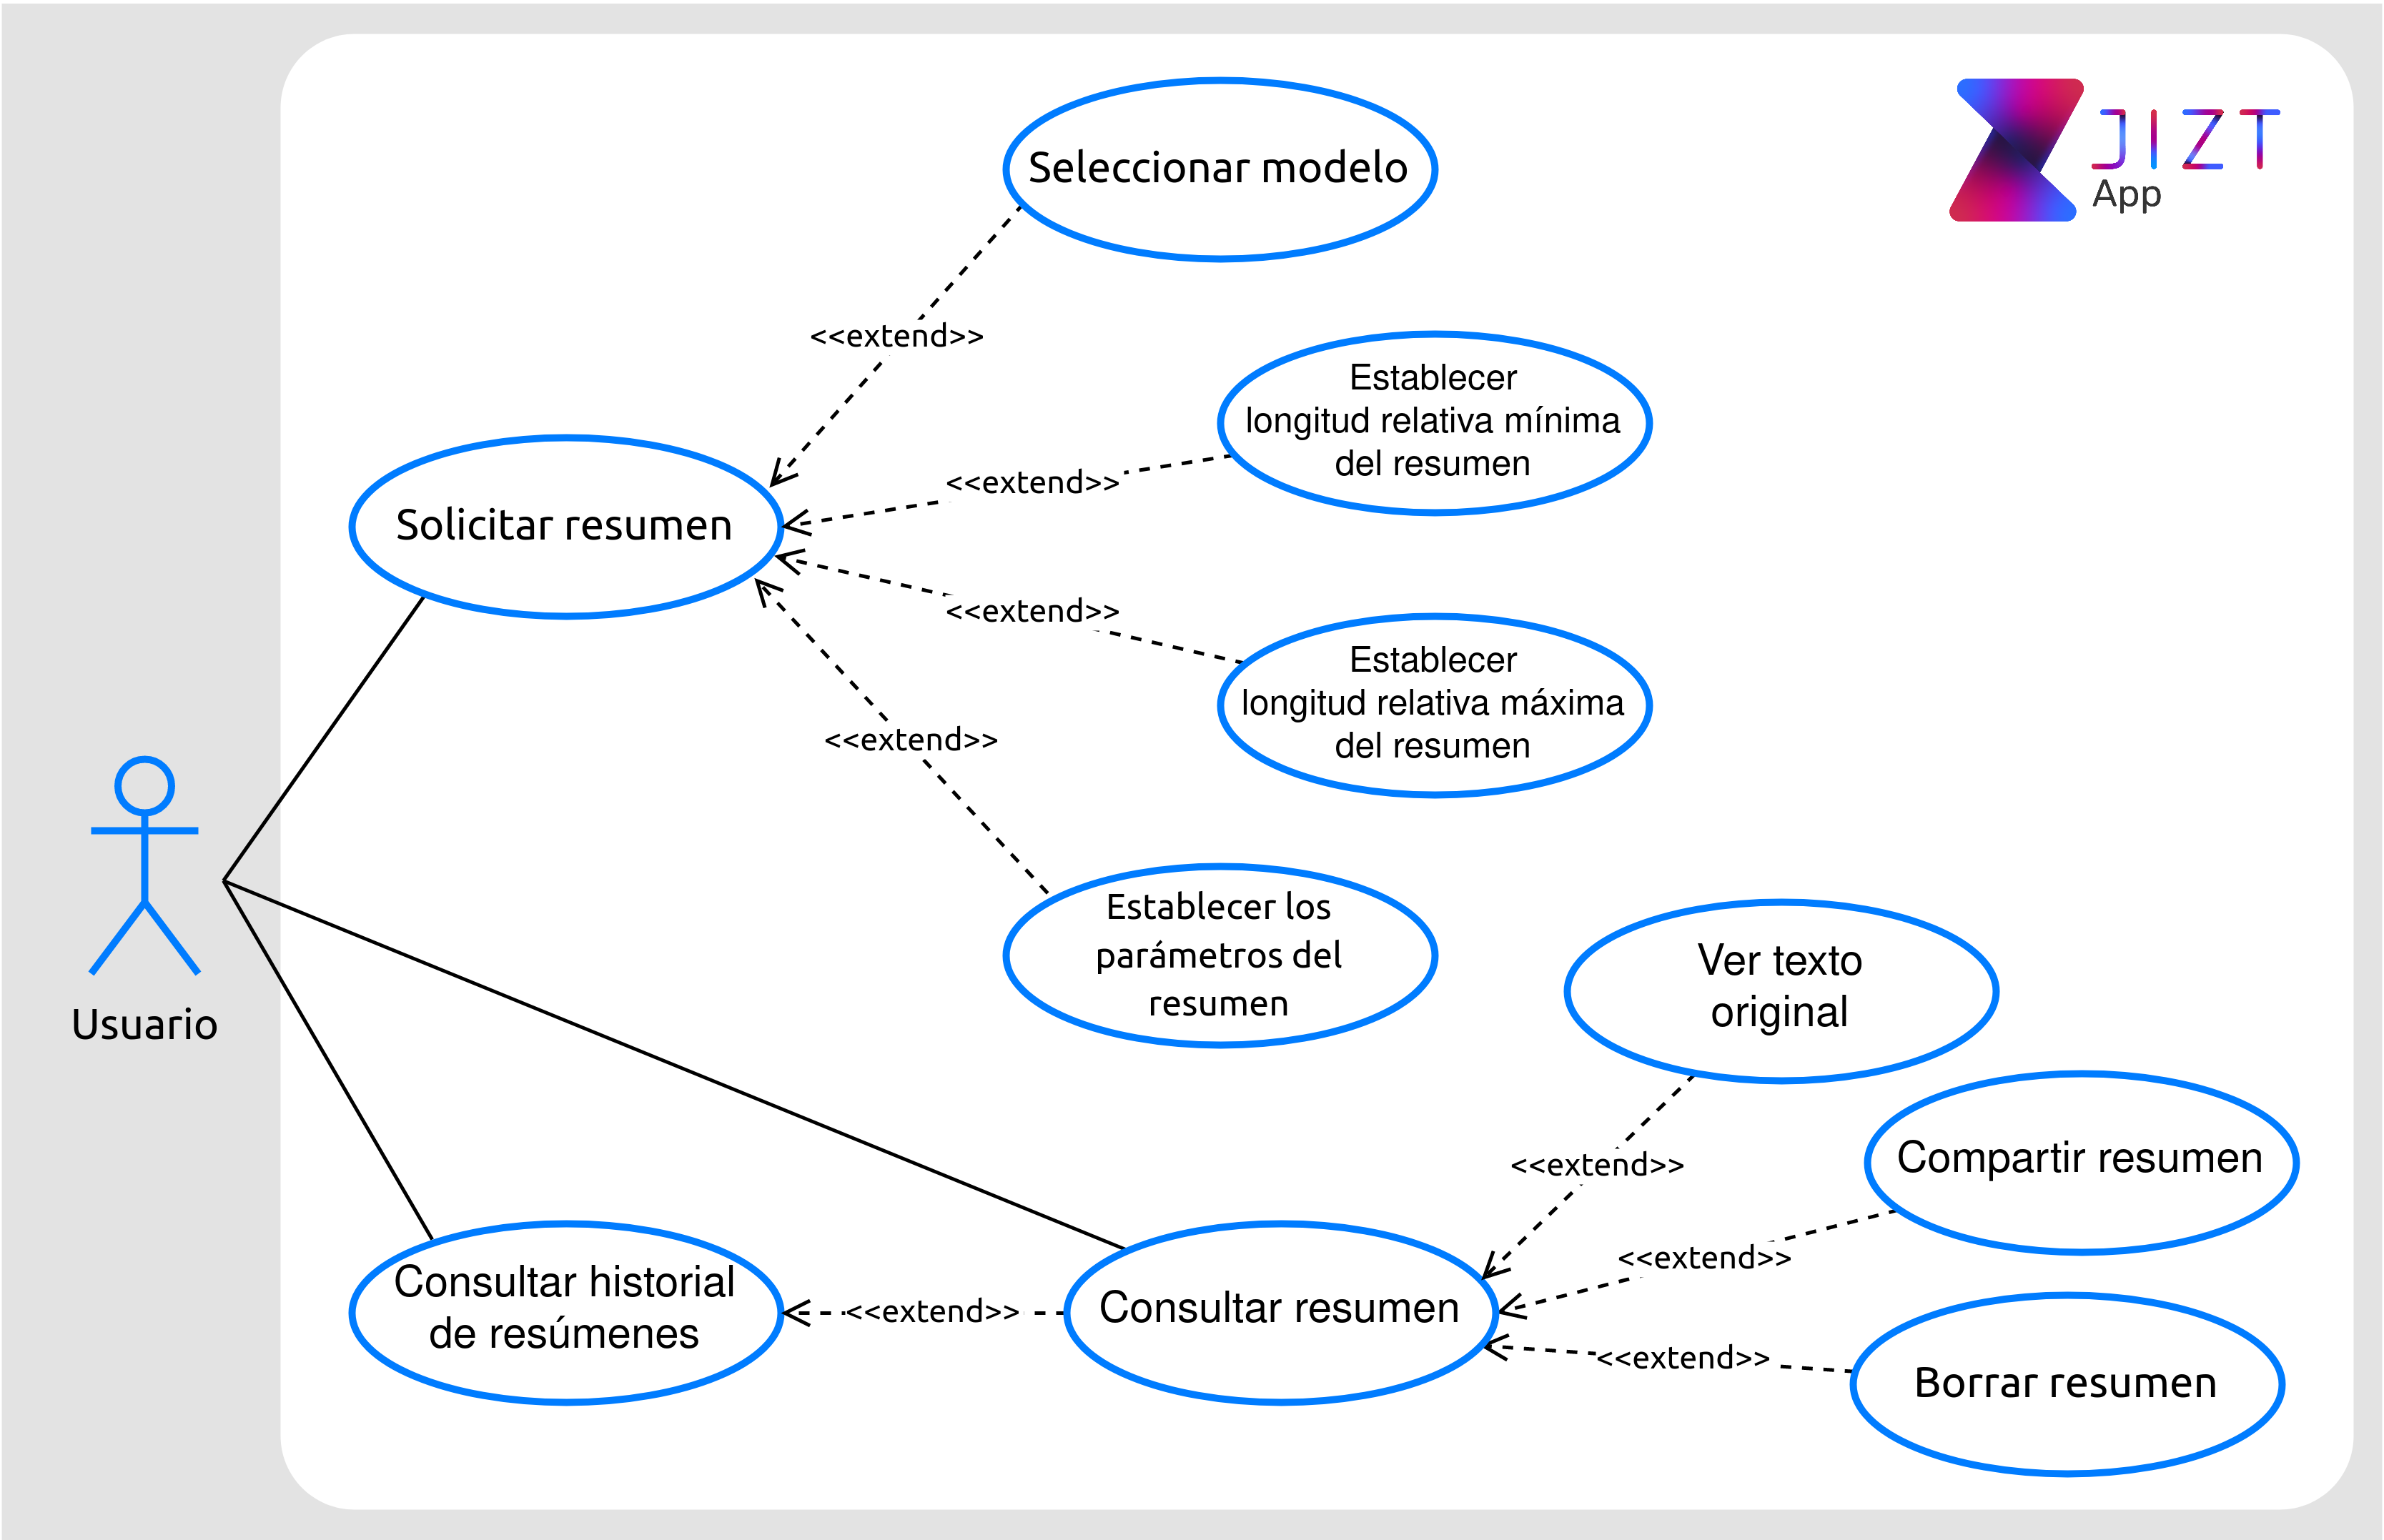
\includegraphics[width=\textwidth]{use-case-diagram}
	\vspace{-0.5cm}
	\caption{Diagrama de casos de uso.}
	\label{flutter-widgets}
\end{figure}

\subsection{Actores}

Existe un único actor: el usuario que hace uso de la aplicación.


\subsection{Casos de uso}

\begin{longtable}{>{\raggedright}b{0.2\linewidth}>{\raggedright\arraybackslash}b{0.7\linewidth}}
	\toprule
	\textbf{CU-01} & \textbf{Solicitar resumen} \\
	\toprule
	\endhead

	\toprule
	\caption{CU-01 Solicitar resumen}
	\endfoot
	
	\small{\textbf{Descripción}} & Solicitar la generación de un resumen a partir de un \\
	& texto. \\
	\small{\textbf{Autor}} & Diego Miguel Lozano \\
	\small{\textbf{Requisitos}} & RF-1, RF-6, RF-8, RF-9 \\
	\small{\textbf{relacionados}} & \\
	\small{\textbf{Precondición}} & La API REST se encuentra accesible. \\
	\small{\textbf{Flujo normal}} & \quad {\small 1. El usuario inicia la aplicación.} \\
	& \quad {\small 2. El usuario hace \emph{click} en} \\
	& \qquad {\small el área de texto.} \\
	& \quad {\small 3. El usuario introduce el texto a resumir o, alterna-} \\
	& \qquad {\small tivamente, lo pega desde el portapapeles.} \\
	& \quad {\small 4. El usuario pulsa en el botón <<Resumir>>.} \\
	& \quad {\small 5. Se muestra un indicador de <<procesando>>.} \\
	& \quad {\small 6. Se muestra un indicador de <<resumen completado>>.} \\
	& \quad {\small 7. Se muestra el resumen generado.} \\
	\small{\textbf{Postcondición}} & El usuario ha obtenido el resumen de su texto. \\
	\small{\textbf{Excepciones}} & API REST inaccesible. \\
	\small{\textbf{Incluye}} & - \\
	\small{\textbf{Extiende}} & - \\
	\small{\textbf{Prioridad}} & Muy alta. \\
	\small{\textbf{Frecuencia de}} & Muy alta. \\
	\small{\textbf{uso}} & \\
	\small{\textbf{Importancia}} & Crítica. \\
	\small{\textbf{Comentarios}} & - \\
\end{longtable}


\begin{longtable}{>{\raggedright}b{0.2\linewidth}>{\raggedright\arraybackslash}b{0.7\linewidth}}
	\toprule
	\textbf{CU-02} & \textbf{Establecer longitud relativa mínima del resumen} \\
	\toprule
	\endhead
	
	\toprule
	\caption{CU-02 Establecer longitud relativa mínima del resumen}
	\endfoot
	
	\small{\textbf{Descripción}} & Establecer la longitud mínima que puede tener el \\
	& resumen generado de manera relativa al texto \\ & original. \\
	\small{\textbf{Autor}} & Diego Miguel Lozano \\
	\small{\textbf{Requisitos}} & RF-1.2  \\
	\small{\textbf{relacionados}} & \\
	\small{\textbf{Precondición}} & - \\
	\small{\textbf{Flujo normal}} & \quad \small{1. El usuario pulsa sobre el cuadro de texto en la} \\
	& \qquad \small{pantalla principal.} \\
	& \quad \small{2. El usuario ajusta la longitud mínima a través del} \\
	& \qquad \small{\emph{slider} que aparece en la parte inferior de la pantalla.} \\
	\small{\textbf{Postcondición}} & Se ha establecido la longitud mínima. \\
	\small{\textbf{Excepciones}} & - \\
	\small{\textbf{Incluye}} & - \\
	\small{\textbf{Extiende}} & - \\
	\small{\textbf{Prioridad}} & Alta. \\
	\small{\textbf{Frecuencia de}} & Alta. \\
	\small{\textbf{uso}} & \\
	\small{\textbf{Importancia}} & Alta. \\
	\small{\textbf{Comentarios}} &  - \\
\end{longtable}

\begin{longtable}{>{\raggedright}b{0.2\linewidth}>{\raggedright\arraybackslash}b{0.7\linewidth}}
	\toprule
	\textbf{CU-03} & \textbf{Establecer longitud relativa máxima del resumen} \\
	\toprule
	\endhead
	
	\toprule
	\caption{CU-03 Establecer longitud relativa máxima del resumen}
	\endfoot
	
	\small{\textbf{Descripción}} & Establecer la longitud máxima que puede tener el \\
	& resumen generado de manera relativa al texto \\ & original. \\
	\small{\textbf{Autor}} & Diego Miguel Lozano \\
	\small{\textbf{Requisitos}} & RF-1.2  \\
	\small{\textbf{relacionados}} & \\
	\small{\textbf{Precondición}} & - \\
	\small{\textbf{Flujo normal}} & \quad \small{1. El usuario pulsa sobre el cuadro de texto en la} \\
	& \qquad \small{pantalla principal.} \\
	& \quad \small{2. El usuario ajusta la longitud máxima a través del} \\
	& \qquad \small{\emph{slider} que aparece en la parte inferior de la pantalla.} \\
	\small{\textbf{Postcondición}} & Se ha establecido la longitud máxima. \\
	\small{\textbf{Excepciones}} & - \\
	\small{\textbf{Incluye}} & - \\
	\small{\textbf{Extiende}} & - \\
	\small{\textbf{Prioridad}} & Alta. \\
	\small{\textbf{Frecuencia de}} & Alta. \\
	\small{\textbf{uso}} & \\
	\small{\textbf{Importancia}} & Alta. \\
	\small{\textbf{Comentarios}} &  - \\
\end{longtable}



\begin{longtable}{>{\raggedright}b{0.2\linewidth}>{\raggedright\arraybackslash}b{0.7\linewidth}}
	\toprule
	\textbf{CU-04} & \textbf{Consultar historial de resúmenes} \\
	\toprule
	\endhead
	
	\toprule
	\caption{CU-04 Consultar historial de resúmenes}
	\endfoot
	
	\small{\textbf{Descripción}} & Visualizar la lista de resúmenes generados previa- \\
	& mente. \\
	\small{\textbf{Autor}} & Diego Miguel Lozano \\
	\small{\textbf{Requisitos}} & RF-2, RF-3, RF-4, RF-5, RF-7  \\
	\small{\textbf{relacionados}} & \\
	\small{\textbf{Precondición}} & Haber generado al menos un resumen previamente. \\
	\small{\textbf{Flujo normal}} & \quad \small{1. El usuario pulsa en <<Ver todos>> en la pantalla princi-} \\
	& \qquad \small{pal.} \\
	& \quad \small{2. Se muestra la lista de resúmenes previos.} \\
	\small{\textbf{Postcondición}} & Se visualizan los resúmenes generados. \\
	\small{\textbf{Excepciones}} & - \\
	\small{\textbf{Incluye}} & - \\
	\small{\textbf{Extiende}} & CU-07 \\
	\small{\textbf{Prioridad}} & Alta. \\
	\small{\textbf{Frecuencia de}} & Alta. \\
	\small{\textbf{uso}} & \\
	\small{\textbf{Importancia}} & Alta. \\
	\small{\textbf{Comentarios}} & Si aún no se ha generado ningún resumen, la lista\\
	& se mostrará vacía. \\
\end{longtable}


\begin{longtable}{>{\raggedright}b{0.2\linewidth}>{\raggedright\arraybackslash}b{0.7\linewidth}}
	\toprule
	\textbf{CU-05} & \textbf{Consultar resumen} \\
	\toprule
	\endhead
	
	\toprule
	\caption{CU-05 Consultar resumen}
	\endfoot
	
	\small{\textbf{Descripción}} & Consultar un resumen generado previamente. \\
	\small{\textbf{Autor}} & Diego Miguel Lozano \\
	\small{\textbf{Requisitos}} & RF-2  \\
	\small{\textbf{relacionados}} & \\
	\small{\textbf{Precondición}} &  Haber generado al menos un resumen previamente. \\
	\small{\textbf{Flujo normal}} & \small{Flujo 1:} \\
	& \quad \small{1. El usuario pulsa en uno de los resúmenes que apa-} \\
	& \qquad \small{recen en el inferior de la pantalla.} \\
	& \small{Flujo 2 (altenativa):} \\
	& \quad \small{1. El usuario pulsa en <<Ver todos>> en la pantalla prin-} \\
	& \qquad \small{cipal.} \\
	& \quad \small{2. Se muestra la lista de resúmenes previos.} \\
	& \quad \small{3. El usuario pulsa en uno de los resúmenes.} \\
	\small{\textbf{Postcondición}} & Se ha mostrado el resumen seleccionado. \\
	\small{\textbf{Excepciones}} & - \\
	\small{\textbf{Incluye}} & -\\
	\small{\textbf{Extiende}} & CU-06 \\
	\small{\textbf{Prioridad}} & Muy alta. \\
	\small{\textbf{Frecuencia de}} & \\
	\small{\textbf{uso}} & Alta. \\
	\small{\textbf{Importancia}} & Crítica. \\
	\small{\textbf{Comentarios}} & - \\
\end{longtable}


\begin{longtable}{>{\raggedright}b{0.2\linewidth}>{\raggedright\arraybackslash}b{0.7\linewidth}}
	\toprule
	\textbf{CU-06} & \textbf{Ver texto original} \\
	\toprule
	\endhead
	
	\toprule
	\caption{CU-06 Ver texto original}
	\endfoot
	
	\small{\textbf{Descripción}} & Visualizar el texto a partir del cual se ha generado \\
	& el resumen. \\
	\small{\textbf{Autor}} & Diego Miguel Lozano \\
	\small{\textbf{Requisitos}} & RF-2, RF-7  \\
	\small{\textbf{relacionados}} & \\
	\small{\textbf{Precondición}} & Haber generado un resumen. \\
	\small{\textbf{Flujo normal}} & \quad \small{1. El usuario pulsa en <<Original>>. } \\
	\small{\textbf{Postcondición}} & Se ha mostrado el texto original.\\
	\small{\textbf{Excepciones}} & - \\
	\small{\textbf{Incluye}} & - \\
	\small{\textbf{Extiende}} & CU-07 \\
	\small{\textbf{Prioridad}} & Alta. \\
	\small{\textbf{Frecuencia de}} & Alta. \\
	\small{\textbf{uso}} & \\
	\small{\textbf{Importancia}} & Crítica. \\
	\small{\textbf{Comentarios}} & - \\
\end{longtable}


\begin{longtable}{>{\raggedright}b{0.2\linewidth}>{\raggedright\arraybackslash}b{0.7\linewidth}}
	\toprule
	\textbf{CU-07} & \textbf{Compartir el resumen} \\
	\toprule
	\endhead
	
	\toprule
	\caption{CU-07 Compartir el resumen}
	\endfoot
	
	\small{\textbf{Descripción}} & Compartir el resumen generado a través de otra \\
	& aplicación. \\
	\small{\textbf{Autor}} & Diego Miguel Lozano \\
	\small{\textbf{Requisitos}} & RF-3  \\
	\small{\textbf{relacionados}} & \\
	\small{\textbf{Precondición}} & Haber generado un resumen. \\
	\small{\textbf{Flujo normal}} & \quad \small{1. El usuario pulsa en el icono de compartir.} \\
	& \quad \small{2. Se muestra una lista de aplicaciones.} \\
	& \quad \small{3. El usuario pulsa en la aplicación a través de la cual} \\
	& \qquad \small{quiere compartir el resumen} \\
	\small{\textbf{Postcondición}} & Se ha compartido el resumen. \\
	\small{\textbf{Excepciones}} & - \\
	\small{\textbf{Incluye}} & - \\
	\small{\textbf{Extiende}} & CU-07 \\
	\small{\textbf{Prioridad}} & Media. \\
	\small{\textbf{Frecuencia de}} & Media. \\
	\small{\textbf{uso}} & \\
	\small{\textbf{Importancia}} & Media. \\
	\small{\textbf{Comentarios}} & - \\
\end{longtable}


\begin{longtable}{>{\raggedright}b{0.2\linewidth}>{\raggedright\arraybackslash}b{0.7\linewidth}}
	\toprule
	\textbf{CU-08} & \textbf{Borrar el resumen} \\
	\toprule
	\endhead
	
	\toprule
	\caption{CU-08 Borrar el resumen}
	\endfoot
	
	\small{\textbf{Descripción}} & Borrar un resumen generado. \\
	\small{\textbf{Autor}} & Diego Miguel Lozano \\
	\small{\textbf{Requisitos}} & RF-5  \\
	\small{\textbf{relacionados}} & \\
	\small{\textbf{Precondición}} & Haber generado un resumen. \\
	\small{\textbf{Flujo normal}} & \quad \small{1. El usuario pulsa en el icono de borrar.} \\
	 & \quad \small{2. Se elimina el resumen y la aplicación vuelve a} \\
	 & \qquad \small{la pantalla principal.} \\
	\small{\textbf{Postcondición}} & Se ha borrado el resumen. \\
	\small{\textbf{Excepciones}} & - \\
	\small{\textbf{Incluye}} & - \\
	\small{\textbf{Extiende}} & CU-07 \\
	\small{\textbf{Prioridad}} & Alta. \\
	\small{\textbf{Frecuencia de}} & Baja. \\
	\small{\textbf{uso}} & \\
	\small{\textbf{Importancia}} & Alta. \\
	\small{\textbf{Comentarios}} & - \\
\end{longtable}
\apendice{Especificación de diseño}

\section{Introducción}

En este apéndice se recogen las características de diseño que implementan los requisitos descritos en el apéndice anterior, a fin de establecer los criterios que se deberán seguir en el desarrollo del sistema.

\section{Elección del nombre del proyecto}

Para la elección del nombre bajo el cual se englobara todo el servicio de resumen de textos en la nube, se consideraron numerosas opciones, de las cuales, las más relevantes fueron:

\vspace{-0.2cm}
\begin{itemize} [\textbullet]
	\item \textbf{Summit}: acrónimo procedente de \emph{Summarize it}. Además, <<\emph{summit}>> tiene el significado de <<cumbre>> o <<cima>> en inglés, sugiriendo el alto rendimiento y potencia del servicio, alcanzando los más \emph{altos} resultados.
	
	\item \textbf{Jizt}: esta palabra, pronunciada en inglés, suena casi idénticamente a <<\emph{gist}>>, la cual se puede traducir como <<esencia>> o <<quid de la cuestión>>.
	
	\item \textbf{Halb}: al revés se lee <<\emph{blah}>> (de \emph{blah, blah, blah}, en inglés) y en alemán significa <<mitad>>, evocando a la idea de resumen. Además se podría ver como una referencia al supercomputador HAL 9000 de la película y posterior novela \emph{2001: Una Odisea del Espacio}.
\end{itemize}

De estas tres, se juzgaron más interesantes las dos últimas; la primera resulta menos original debido a que ya existen numerosas empresas, productos y proyectos con este nombre.

En ese momento, se llevó a cabo una pequeña encuesta para determinar el nombre final. Dado que el proyecto aspira a tener un carácter internacional, el objetivo de la encuesta no era tanto obtener un gran numero de votaciones, sino que las que tuviéramos fueran muy variada: en total se preguntó a 22 personas de 15 nacionalidades diferentes.

A continuación, se incluye una tabla resumiendo los resultados de la encuesta:

\vspace{0.5cm}
\begin{table}[h]
	\centering
	\begin{tabular}{>{\raggedright}b{0.168\textwidth}>{\centering}b{0.2\textwidth}>{\centering\arraybackslash}b{0.2\textwidth}}
		\toprule
		\multicolumn{3}{c}{\large\textbf{Elección de Nombre}} \\
		\smallskip
		& \textbf{\emph{jizt}} & \textbf{\emph{halb}} \\
		\midrule
		\small{España} & \small{2} & \small{3} \\
		\small{Alemania} & \small{3} & \small{0} \\
		\small{México} & \small{1} & \small{1} \\
		\small{Taiwán} & \small{1} & \small{0} \\
		\small{Japón} & \small{0} & \small{1} \\
		\small{Escocia} & \small{0} & \small{1} \\
		\small{China} & \small{0} & \small{1} \\
		\small{Francia} & \small{0} & \small{1} \\
		\small{Turquía} & \small{0} & \small{1} \\
		\small{Vietnam} & \small{1} & \small{0} \\
		\small{Hungría} & \small{1} & \small{0} \\
		\small{Bielorrusia} & \small{1} & \small{0} \\
		\small{Corea del Sur} & \small{1} & \small{0} \\
		\small{Malasia} & \small{1} & \small{0} \\
		\small{Serbia} & \small{1} & \small{0} \\
		\midrule
		\textbf{\hspace{0.025\textwidth}Total} & \textbf{13} & \textbf{9} \\
		\bottomrule
	\end{tabular}
	\caption{Resultados de la encuesta.}
\end{table}

Aunque los resultados de la encuesta estuvieron bastante ajustados, finalmente la balanza se decantó del lado de JIZT. Algunos de los participantes destacaron su <<sonido vibrante y moderno>>. Por otro lado, el término Halb pareció no convencer a los alemanes, quienes la veían como una palabra demasiado convencional (recordamos que en alemán tiene el significado de <<mitad>>).

\newpage

\section{Diseño de datos}

JIZT comprende dos dominios independientes: el \emph{backend} y el \emph{frontend}. El primero, el \emph{backend}, incluye la API REST, así como los diferentes microservicios que hacen posible la generación de resúmenes en la nube. A su vez, el \emph{frontend} está conformado por la aplicación multiplataforma que se comunica con el \emph{backend} para proporcionar los resúmenes a los usuarios.

Dado que, como decíamos, el diseño de datos es independiente en el caso del \emph{backend} y del \emph{frontend} (siempre que se introduzcan mecanismos para transformar los datos de un dominio al otro, el cual es nuestro caso), atenderemos a cada uno de estos diseños por separado.

\subsubsection{\Large \emph{Backend}}

El \emph{backend} sigue una arquitectura de microservicios. Debido a la propia naturaleza de esta arquitectura, cada uno de estos microservicios tiene una implementación independiente del resto.

Por tanto debemos atender a las clases y sus relaciones en cada microservicio por separado. No obstante, existen dos clases que van a aparecer en todos los microservicios. Se trata de las clases relacionadas con Kafka, esto es, el consumidor y el productor\footnote{\, Para más información sobre Kafka, se recomienda acudir al capítulo de <<Técnicas y herramientas>> de la Memoria.}:

\vspace{-0.2cm}
\begin{itemize} [\textbullet]
	\item \textbf{Productor de Kafka (\emph{Producer})}:  esta clase contiene la lógica que posibilita el envío los mensajes correspondientes a uno o varios Kafka \emph{topics}. Los Kafka \emph{topics} concretos a los que envía el mensaje varían en función del microservicio.
	
	\item \textbf{Consumidor de Kafka (\emph{Consumer})}: un consumidor presta atención constante a los \emph{topics} a los que está subscrito, y en el caso de que se haya producido algún mensaje, lo consume.  Los Kafka \emph{topics} concretos a los que un consumidor está subscrito varían en función del microservicio.
\end{itemize}

Una vez introducidas estas dos clases comunes, veamos las clases concretas de cada microservicio.

\newpage

\noindent
\textbf{\large Microservicio \emph{Dispatcher}}

El \emph{Dispatcher} se encarga de recibir las peticiones de los clientes, validarlas, y reenviarlas hacia el microservicio correspondiente. Como tal, implementa la API REST.

Este microservicio cuenta con las siguientes clases:

\vspace{-0.2cm}
\begin{itemize} [\textbullet]
	\item \textbf{Servicio \emph{Dispatcher} (\emph{DispatcherService})}: clase principal del microservicio. Dirige las interacciones entre las instancias del resto de clases.
	\item \textbf{Resumen (\emph{Summary)}}: se trata de la representación de un resumen, por lo que es una de las clases centrales en todo el proyecto. Entre sus campos más importantes se encuentran su \emph{id}, el cual permite identificar inequívocamente un resumen, así como el texto del propio resumen, y el texto fuente a partir del cual se ha generado el resumen.
	
	\item \textbf{Interfaz Resumen DAO (\emph{SummaryDAOInterface})}: interfaz DAO (\emph{Data Access Object}) para abstraer el acceso a los datos independientemente de la base de datos empleada.
	
	\item \textbf{Factoría Resumen DAO (\emph{SummaryDAOFactory})}: clase que recoge las instancias particulares de los DAOs correspondientes cada base de datos.
	
	\item \textbf{PostgreSQL DAO Resumen (\emph{SummaryDAOPostgresql})}: DAO concreto para la base de datos PostgreSQL. esta base de datos almacena los resúmenes generados.

	\item \textbf{Esquema para Petición de Texto Plano (\emph{PlainTextRequestSchema})}: esta clase contiene la estructura (campos) que debe seguir el cuerpo de las peticiones HTTP de los clientes a la hora de realizar una operación POST sobre la API REST. Se incluye la distinción de <<texto plano>>, dado que en un futuro se podrán realizar peticiones enviando una URL o un documento, y por lo tanto necesitaremos otro esquema diferente para cada uno de estos casos. Este esquema se emplea también para los mensajes producidos por el \emph{Dispatcher} al \emph{topic} del \emph{Pre-procesador} (el siguiente microservicio).
	
	\item \textbf{Esquema para Respuesta (\emph{ResponseSchema})}: estructura (campos) del cuerpo de la respuesta HTTP de la API REST ante una petición POST o GET por parte del cliente. Contiene los detalles del resumen producido.
	
	\item \textbf{Esquema para Mensajes Consumidos \\ (\emph{TextPostprocessingConsumedMsgSchema})}: estructura (campos) que presenta un mensaje consumido por el \emph{Disptacher}. Estos mensajes procederán del \emph{topic} del microservicio Post-procesador de textos.
\end{itemize}

\noindent
\textbf{Diagrama de clases}

\begin{figure}[h]
	\centering
	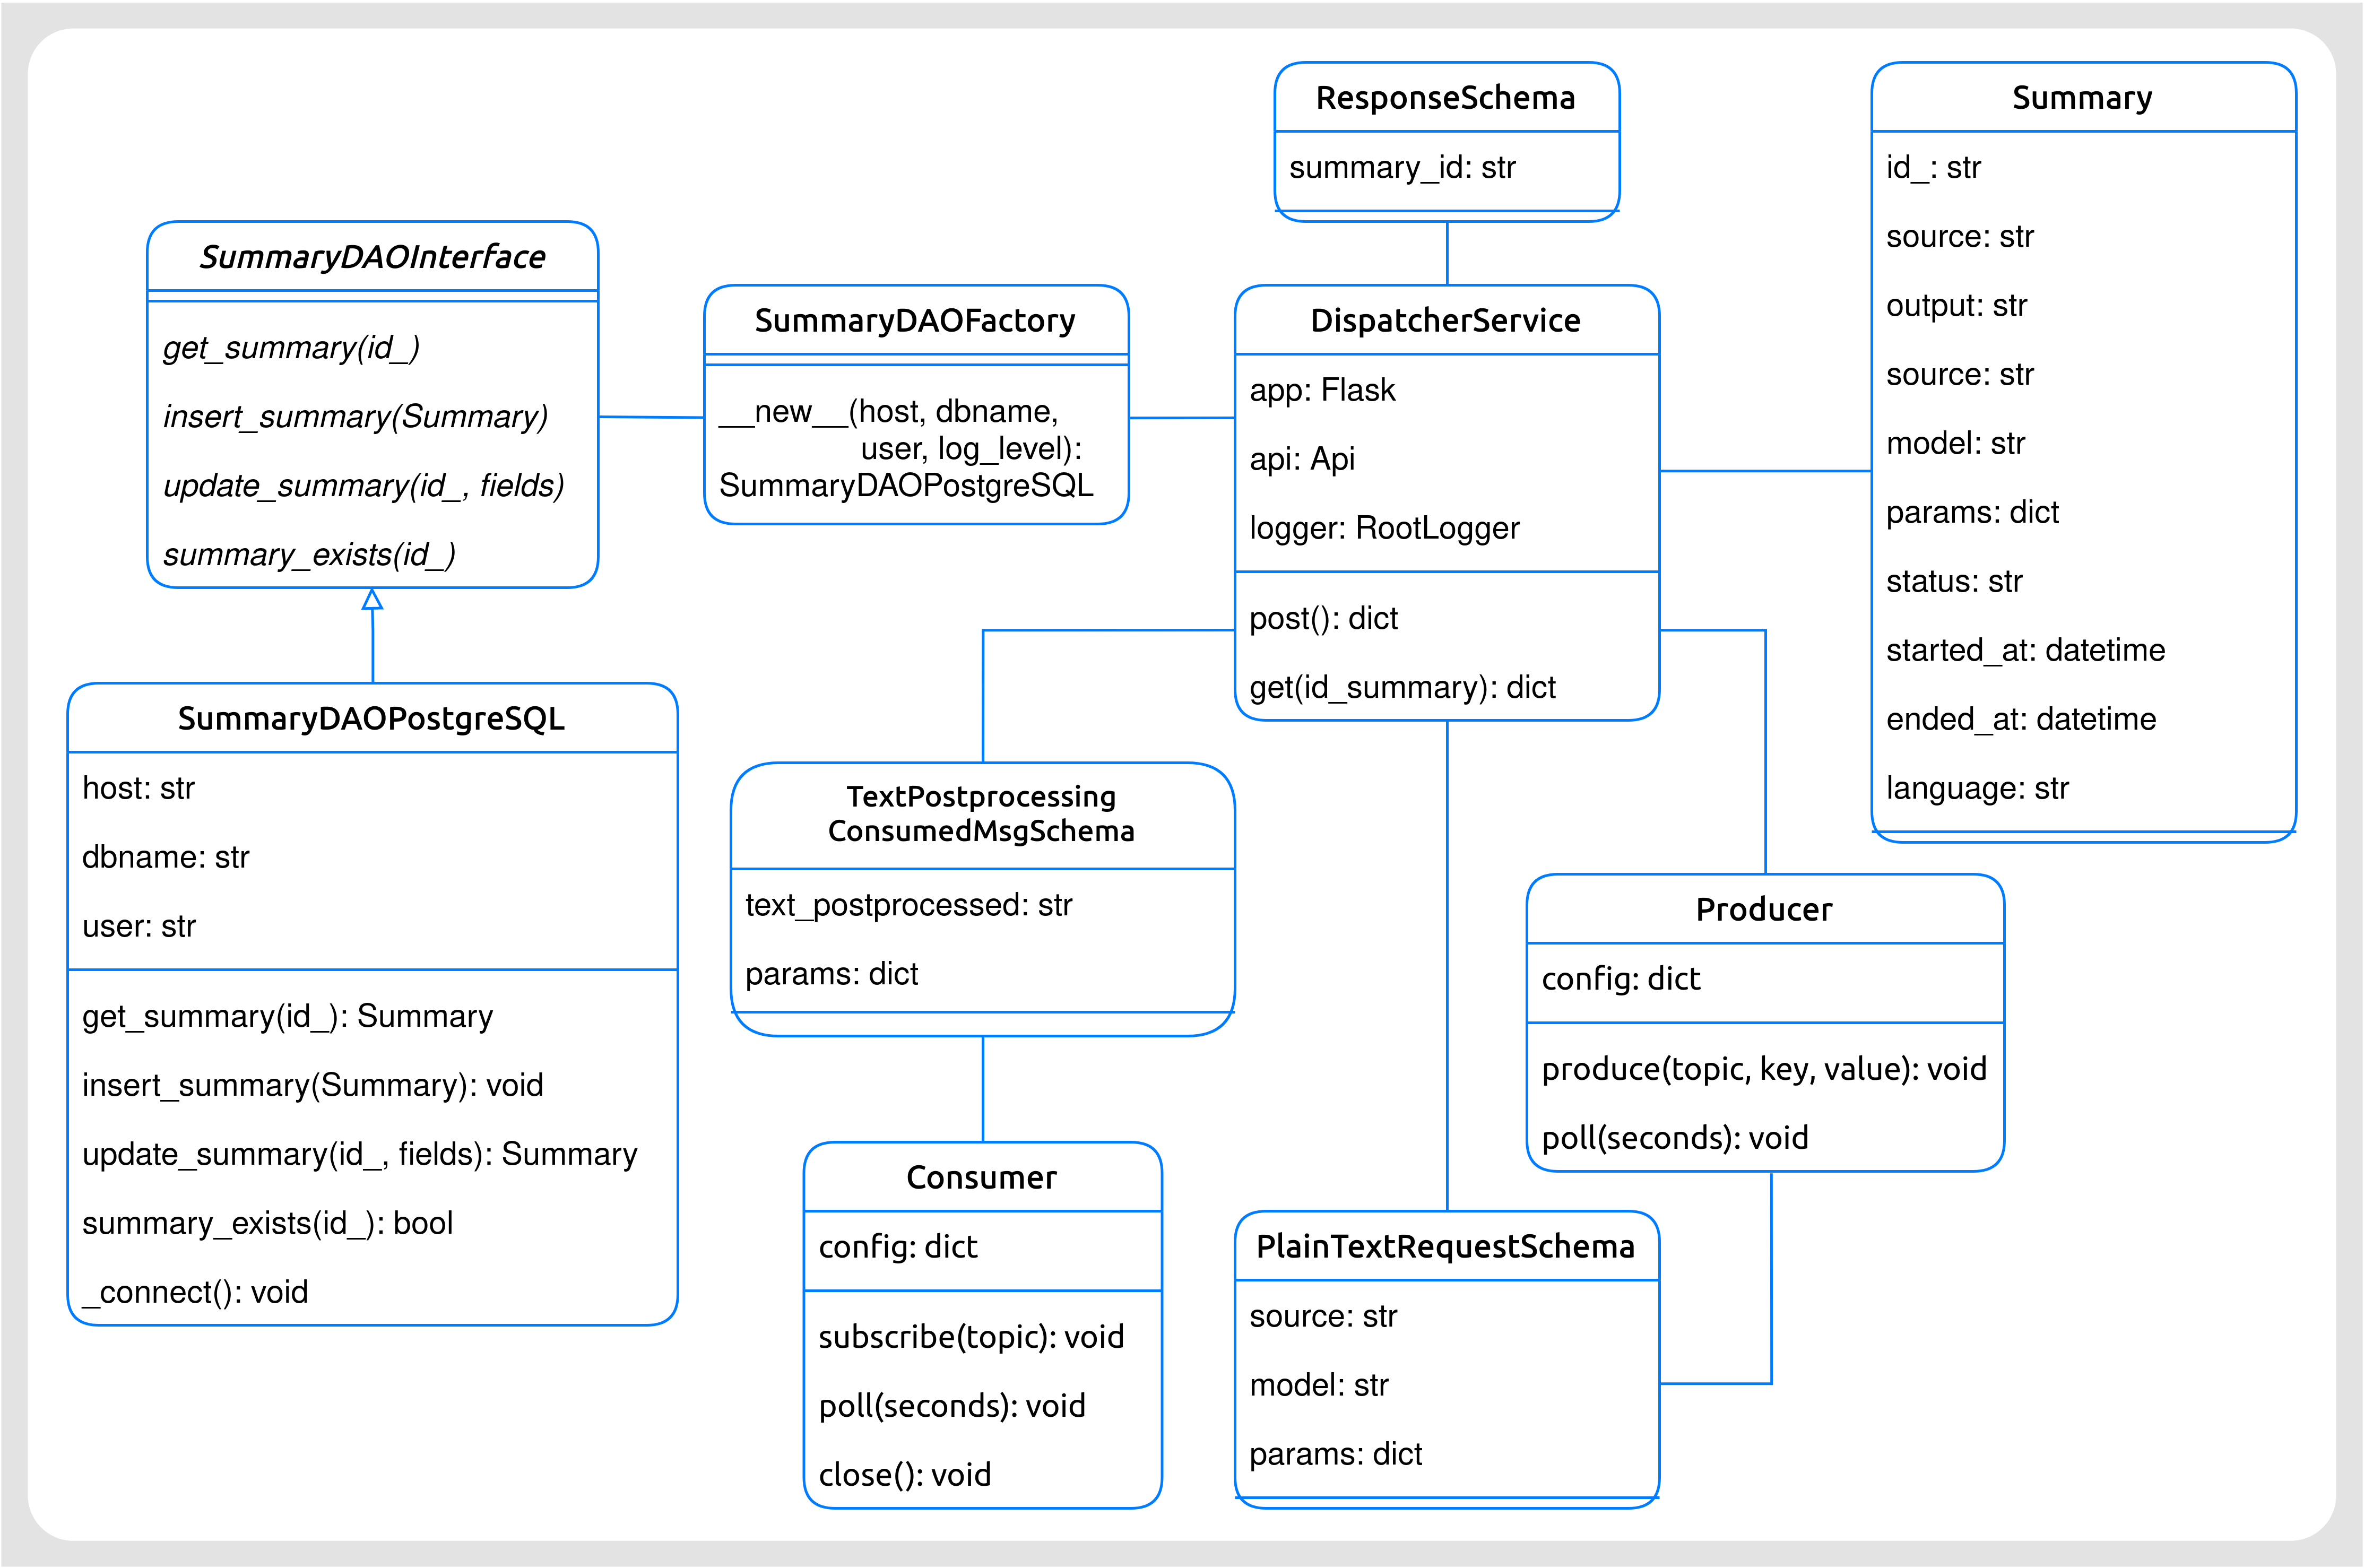
\includegraphics[width=\textwidth]{classes-dispatcher}
	\vspace{-0.5cm}
	\caption{Diagrama de clases del \emph{Dispatcher}.}
\end{figure}

\newpage

\noindent
\textbf{Diagrama E/R de la base de datos}

\begin{figure}[h!]
	\centering
	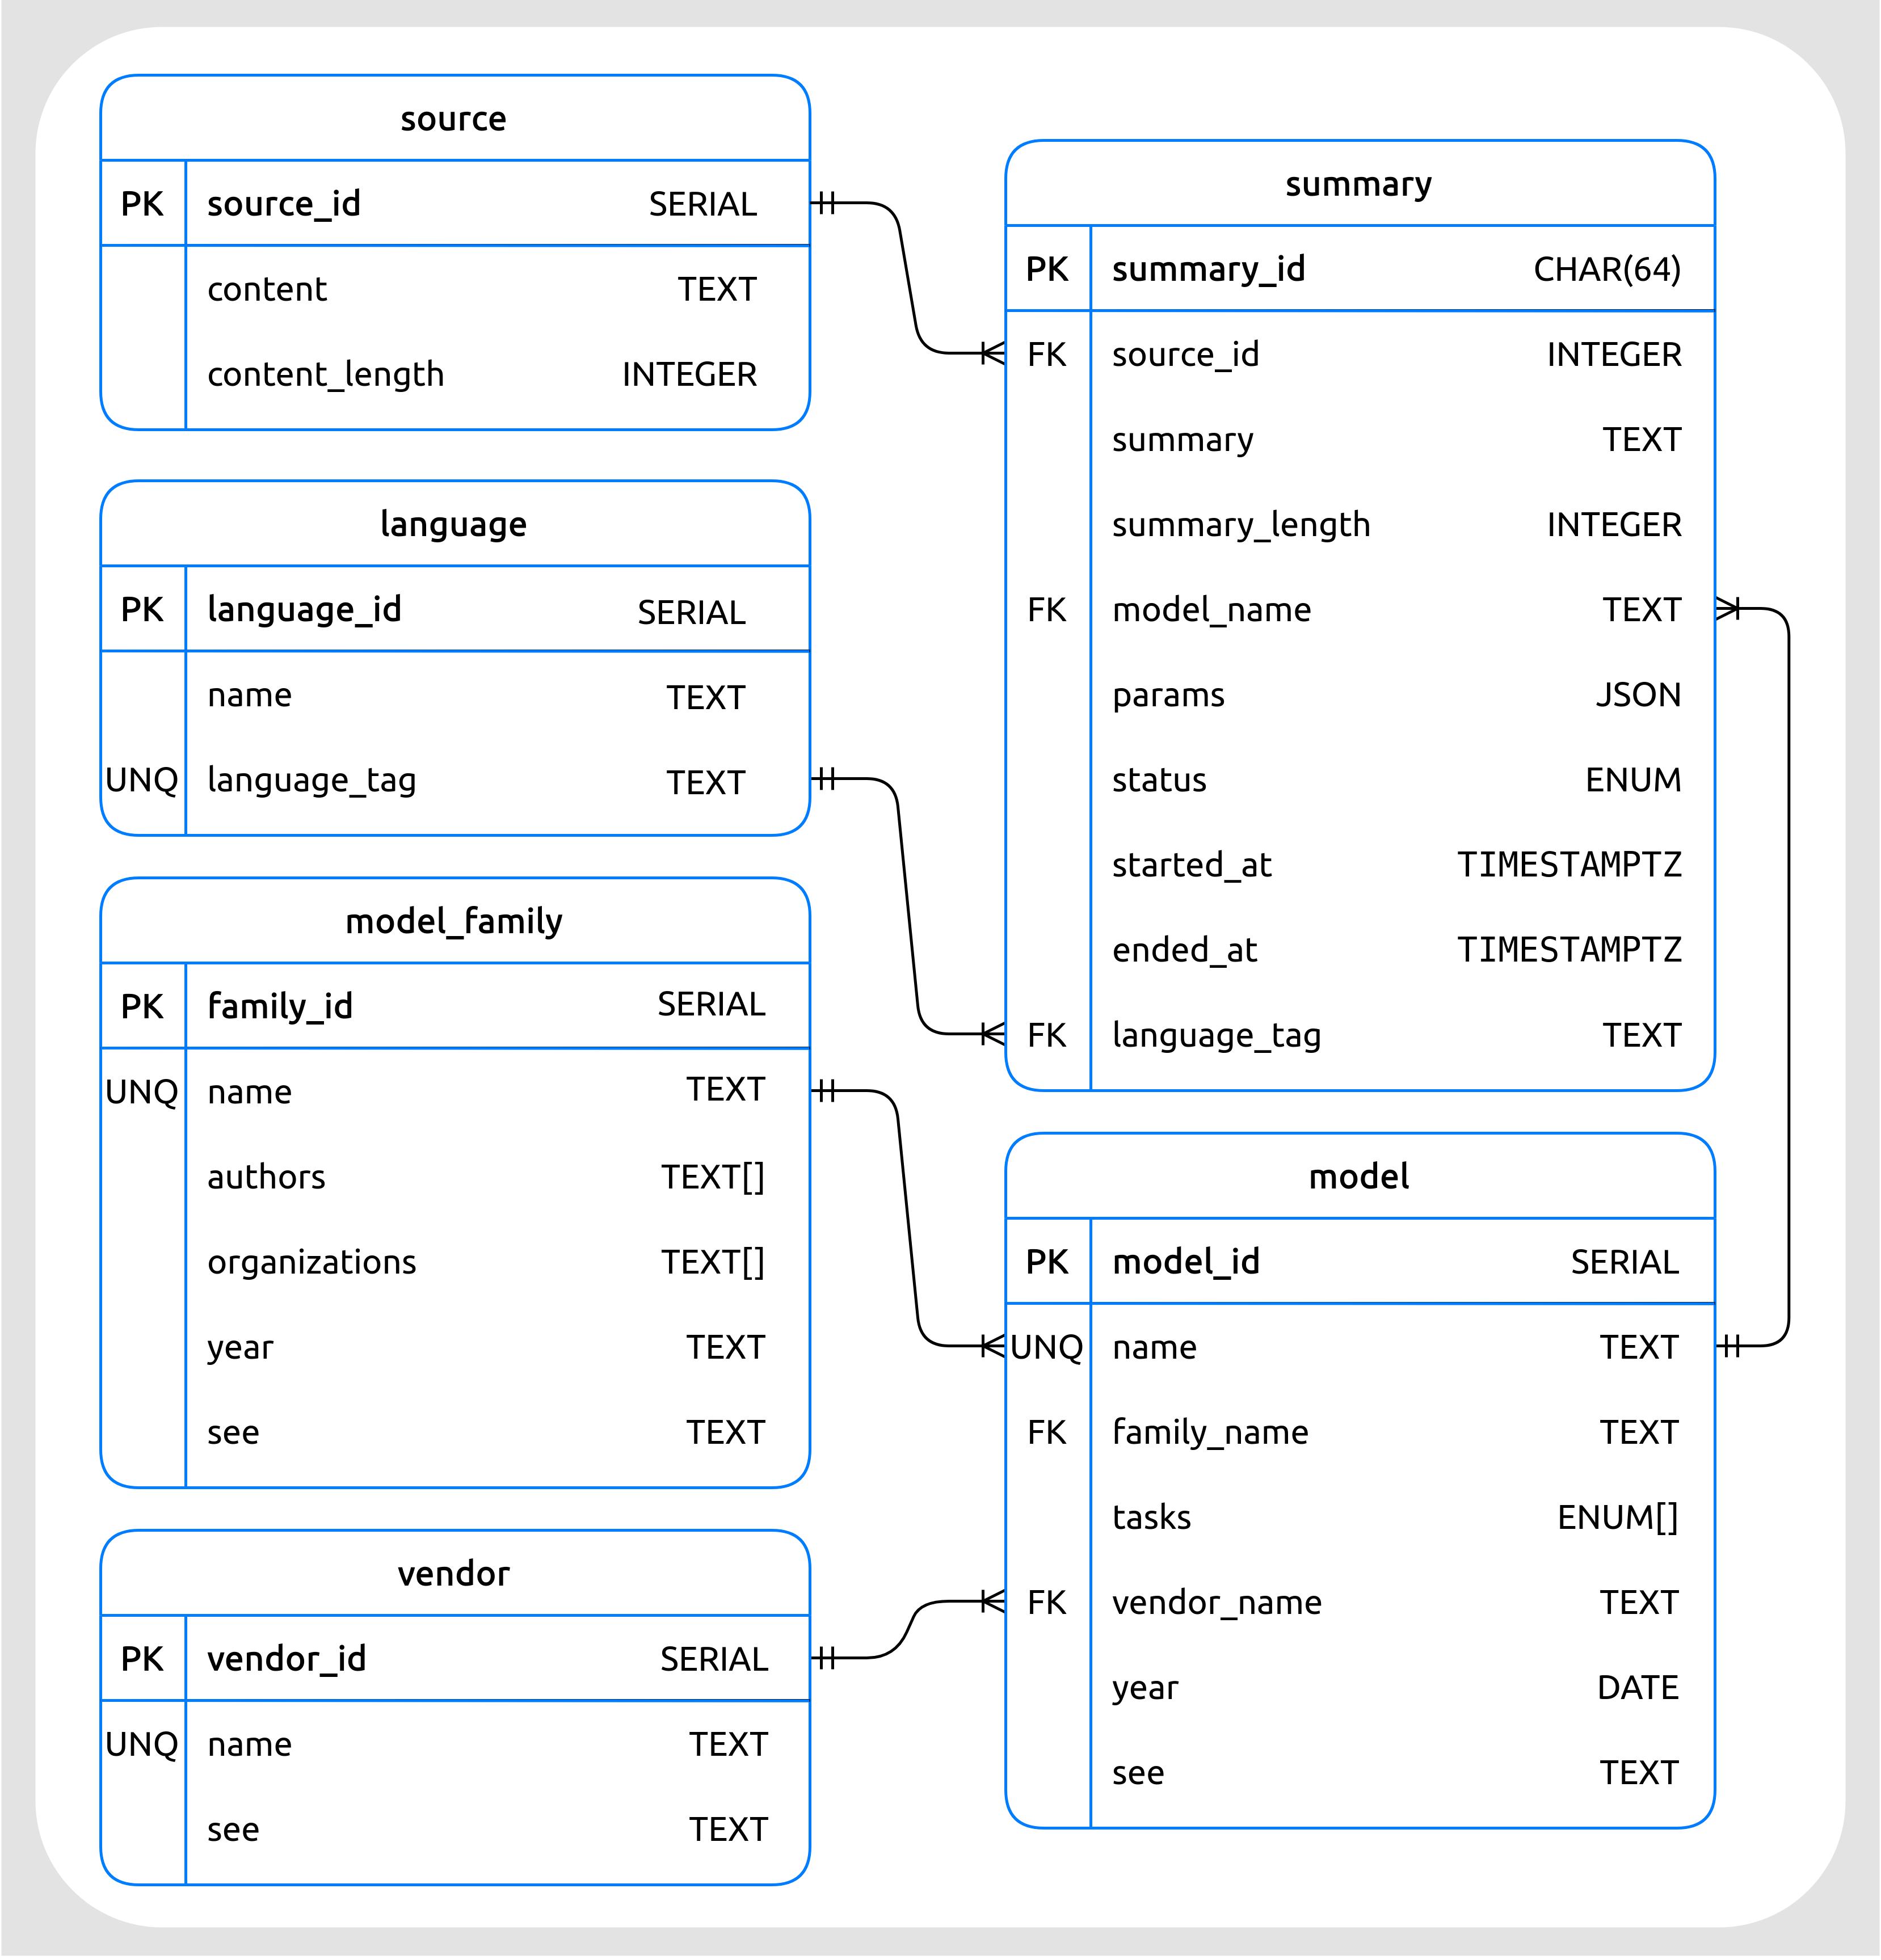
\includegraphics[width=\textwidth]{dispatcher-db}
	\vspace{-0.5cm}
	\caption{Diagrama E/R de la base de datos (tipos de datos de PostgreSQL).}
\end{figure}


\noindent
\textbf{\large Microservicio Pre-procesador de textos}

El Pre-procesador se encarga de realizar un primer procesado de los textos de entrada, a fin de que sean lo más cercanos como sea posible a la entrada que espera el modelo generador de resúmenes.

Este microservicio está compuesto por siguientes clases:

\vspace{-0.2cm}
\begin{itemize} [\textbullet]
	\item \textbf{Pre-procesador de textos (\emph{TextPreprocessor})}: esta clase es la encargada de realizar el pre-procesado del texto.
	
	\item \textbf{Esquema para Mensajes Consumidos \\ (\emph{TextPreprocessingConsumedMsgSchema})}: estructura (campos) que presenta un mensaje consumido por el Pre-procesador. Estos mensajes procederán del microservicio \emph{Dispatcher}.
	
	\item \textbf{Esquema para Mensajes Producidos \\ (\emph{TextEncodingProducedMsgSchema})}: estructura (campos) que presenta un mensaje producido al \emph{topic} del siguiente microservicio (el Codificador de textos).
\end{itemize}

\noindent
\textbf{Diagrama de clases}

\begin{figure}[h]
	\centering
	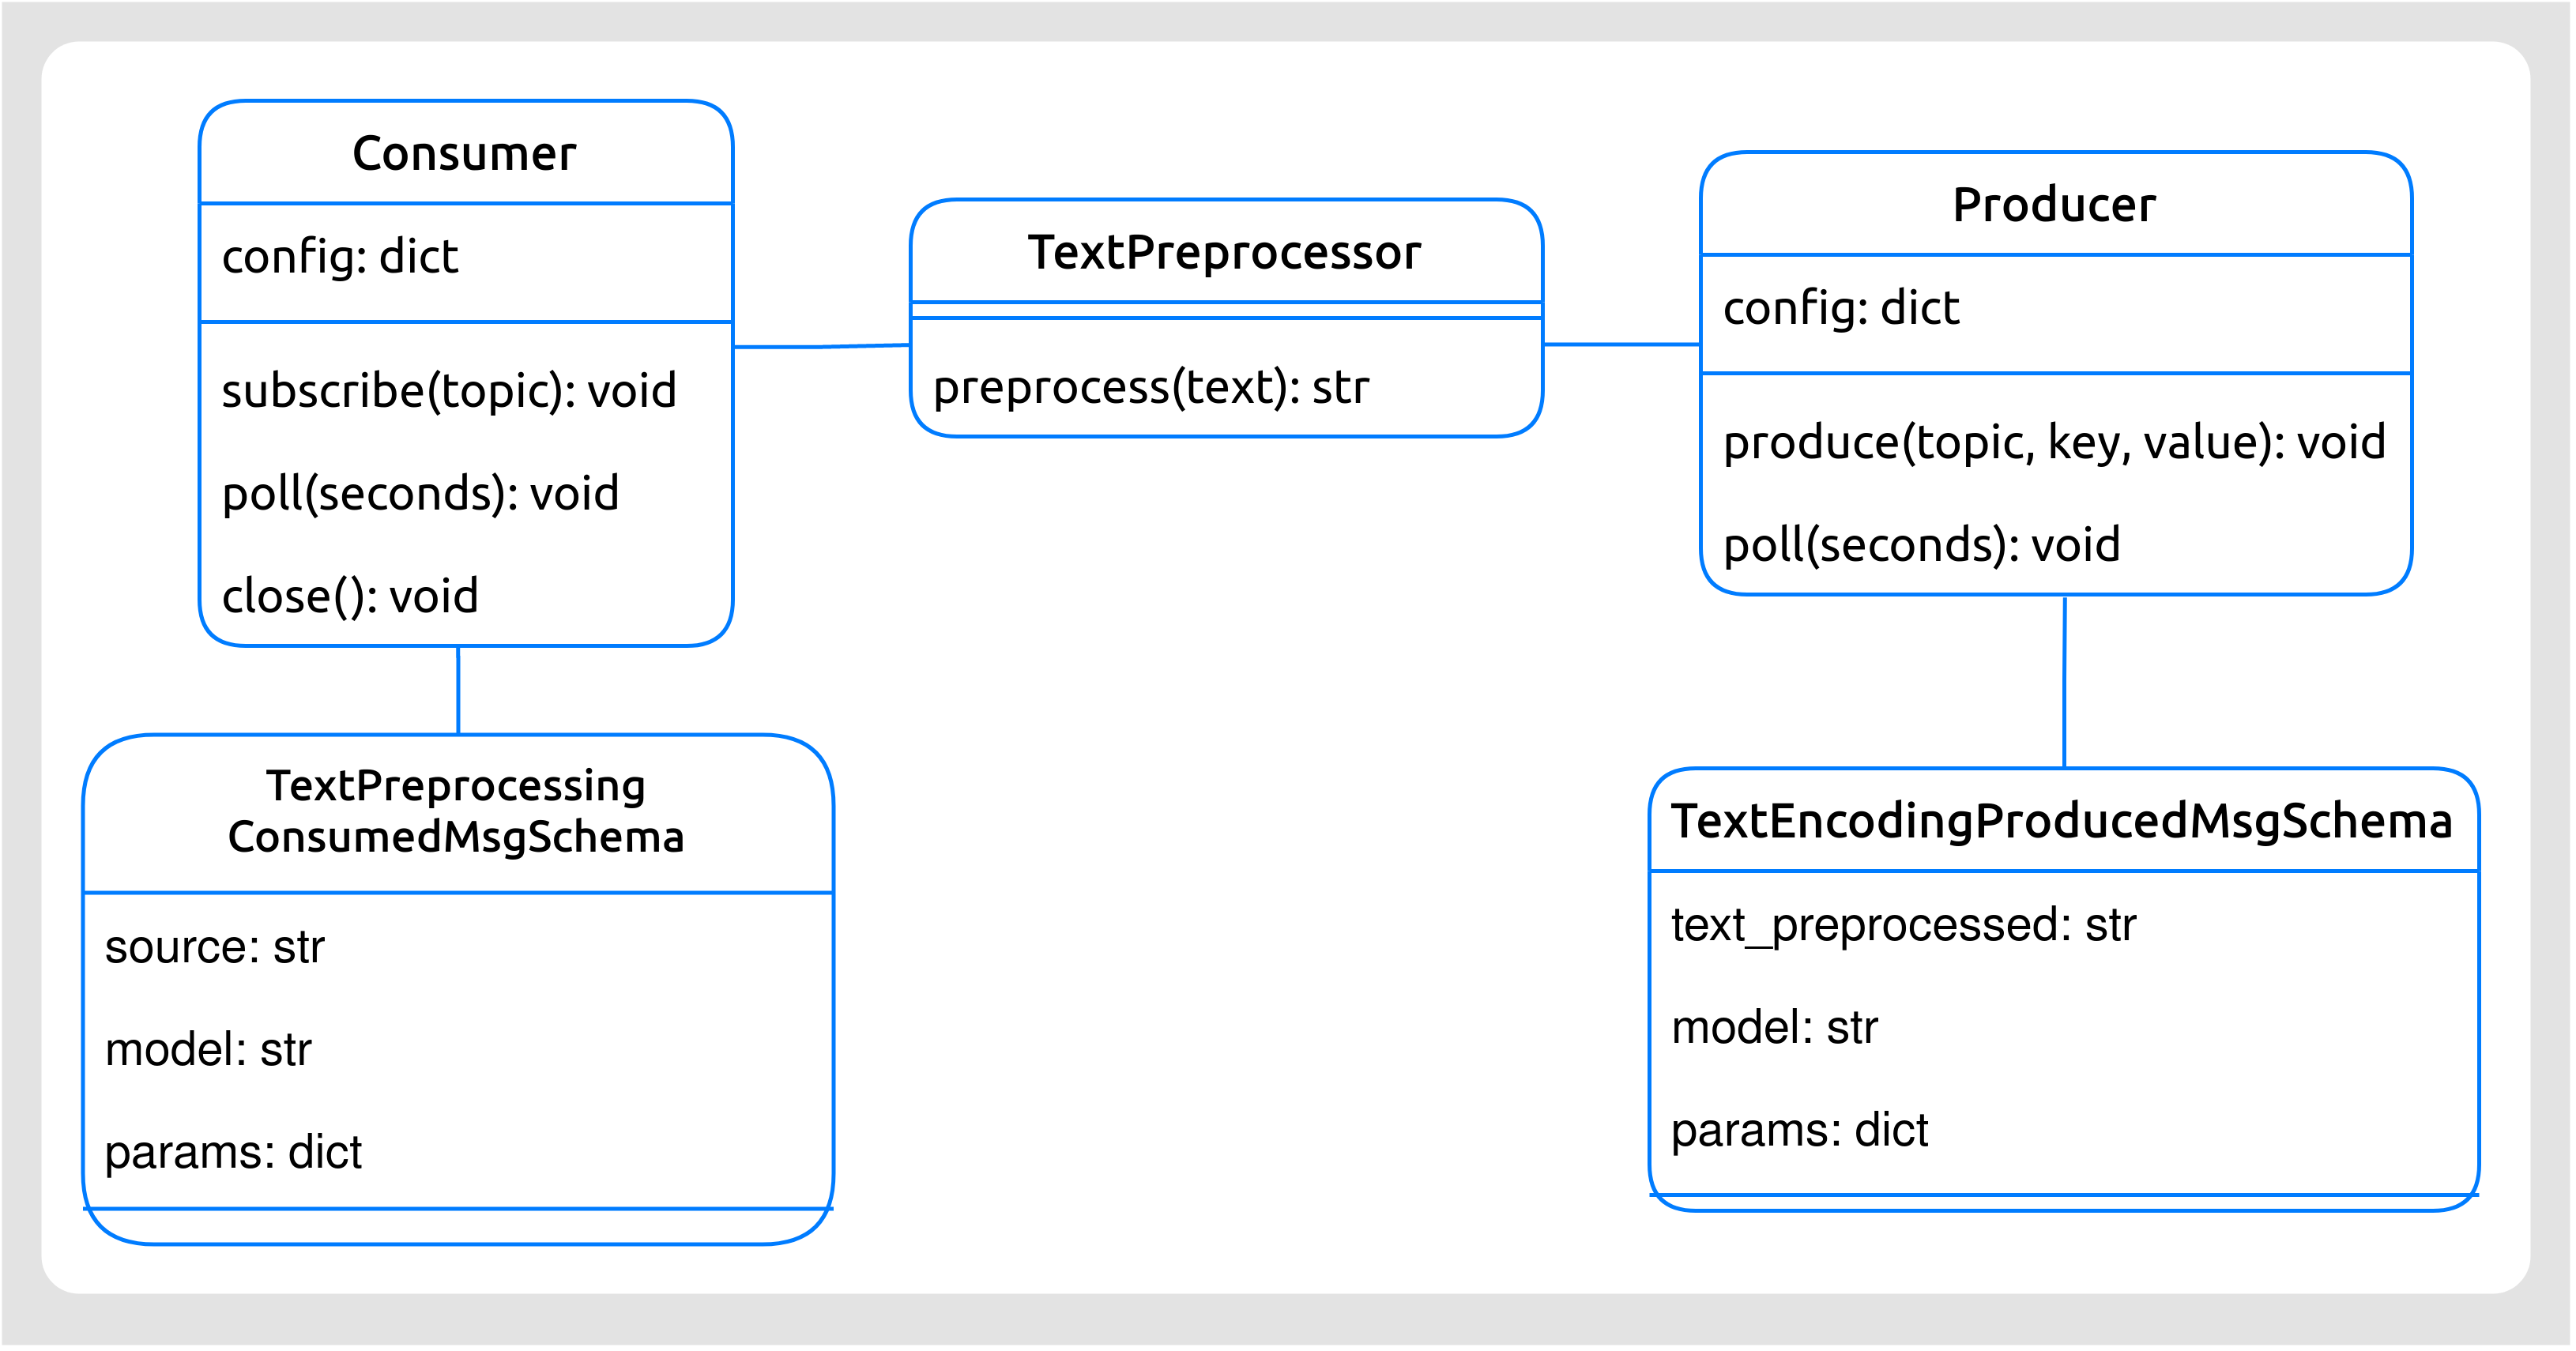
\includegraphics[width=\textwidth]{classes-preprocessor}
	\vspace{-0.5cm}
	\caption{Diagrama de clases del Pre-procesador de textos.}
\end{figure}


\noindent
\textbf{\large Microservicio Codificador de textos}

Este microservicio se encarga de codificar el texto y dividirlo en fragmentos menores, a fin de respetar la longitud máxima de entrada del modelo generador de resúmenes.

El Codificador cuenta con las siguientes clases:

\vspace{-0.2cm}
\begin{itemize} [\textbullet]
	\item \textbf{Codificador y divisor de textos (\emph{SplitterEncoder})}: esta clase es la encargada de realizar el codificado y división del texto.
	
	\item \textbf{Esquema para Mensajes Consumidos \\ (\emph{TextEncodingsConsumedMsgSchema})}: estructura (campos) que presenta un mensaje consumido por el Codificador. Estos mensajes procederán del microservicio Pre-procesador de textos.
	
	\item \textbf{Esquema para Mensajes Producidos \\ (\emph{TextSumarizationProducedMsgSchema})}: estructura (campos) que presenta un mensaje producido al \emph{topic} del siguiente microservicio (el Generador de resumen).
\end{itemize}

\noindent
\textbf{Diagrama de clases}

\begin{figure}[h]
	\centering
	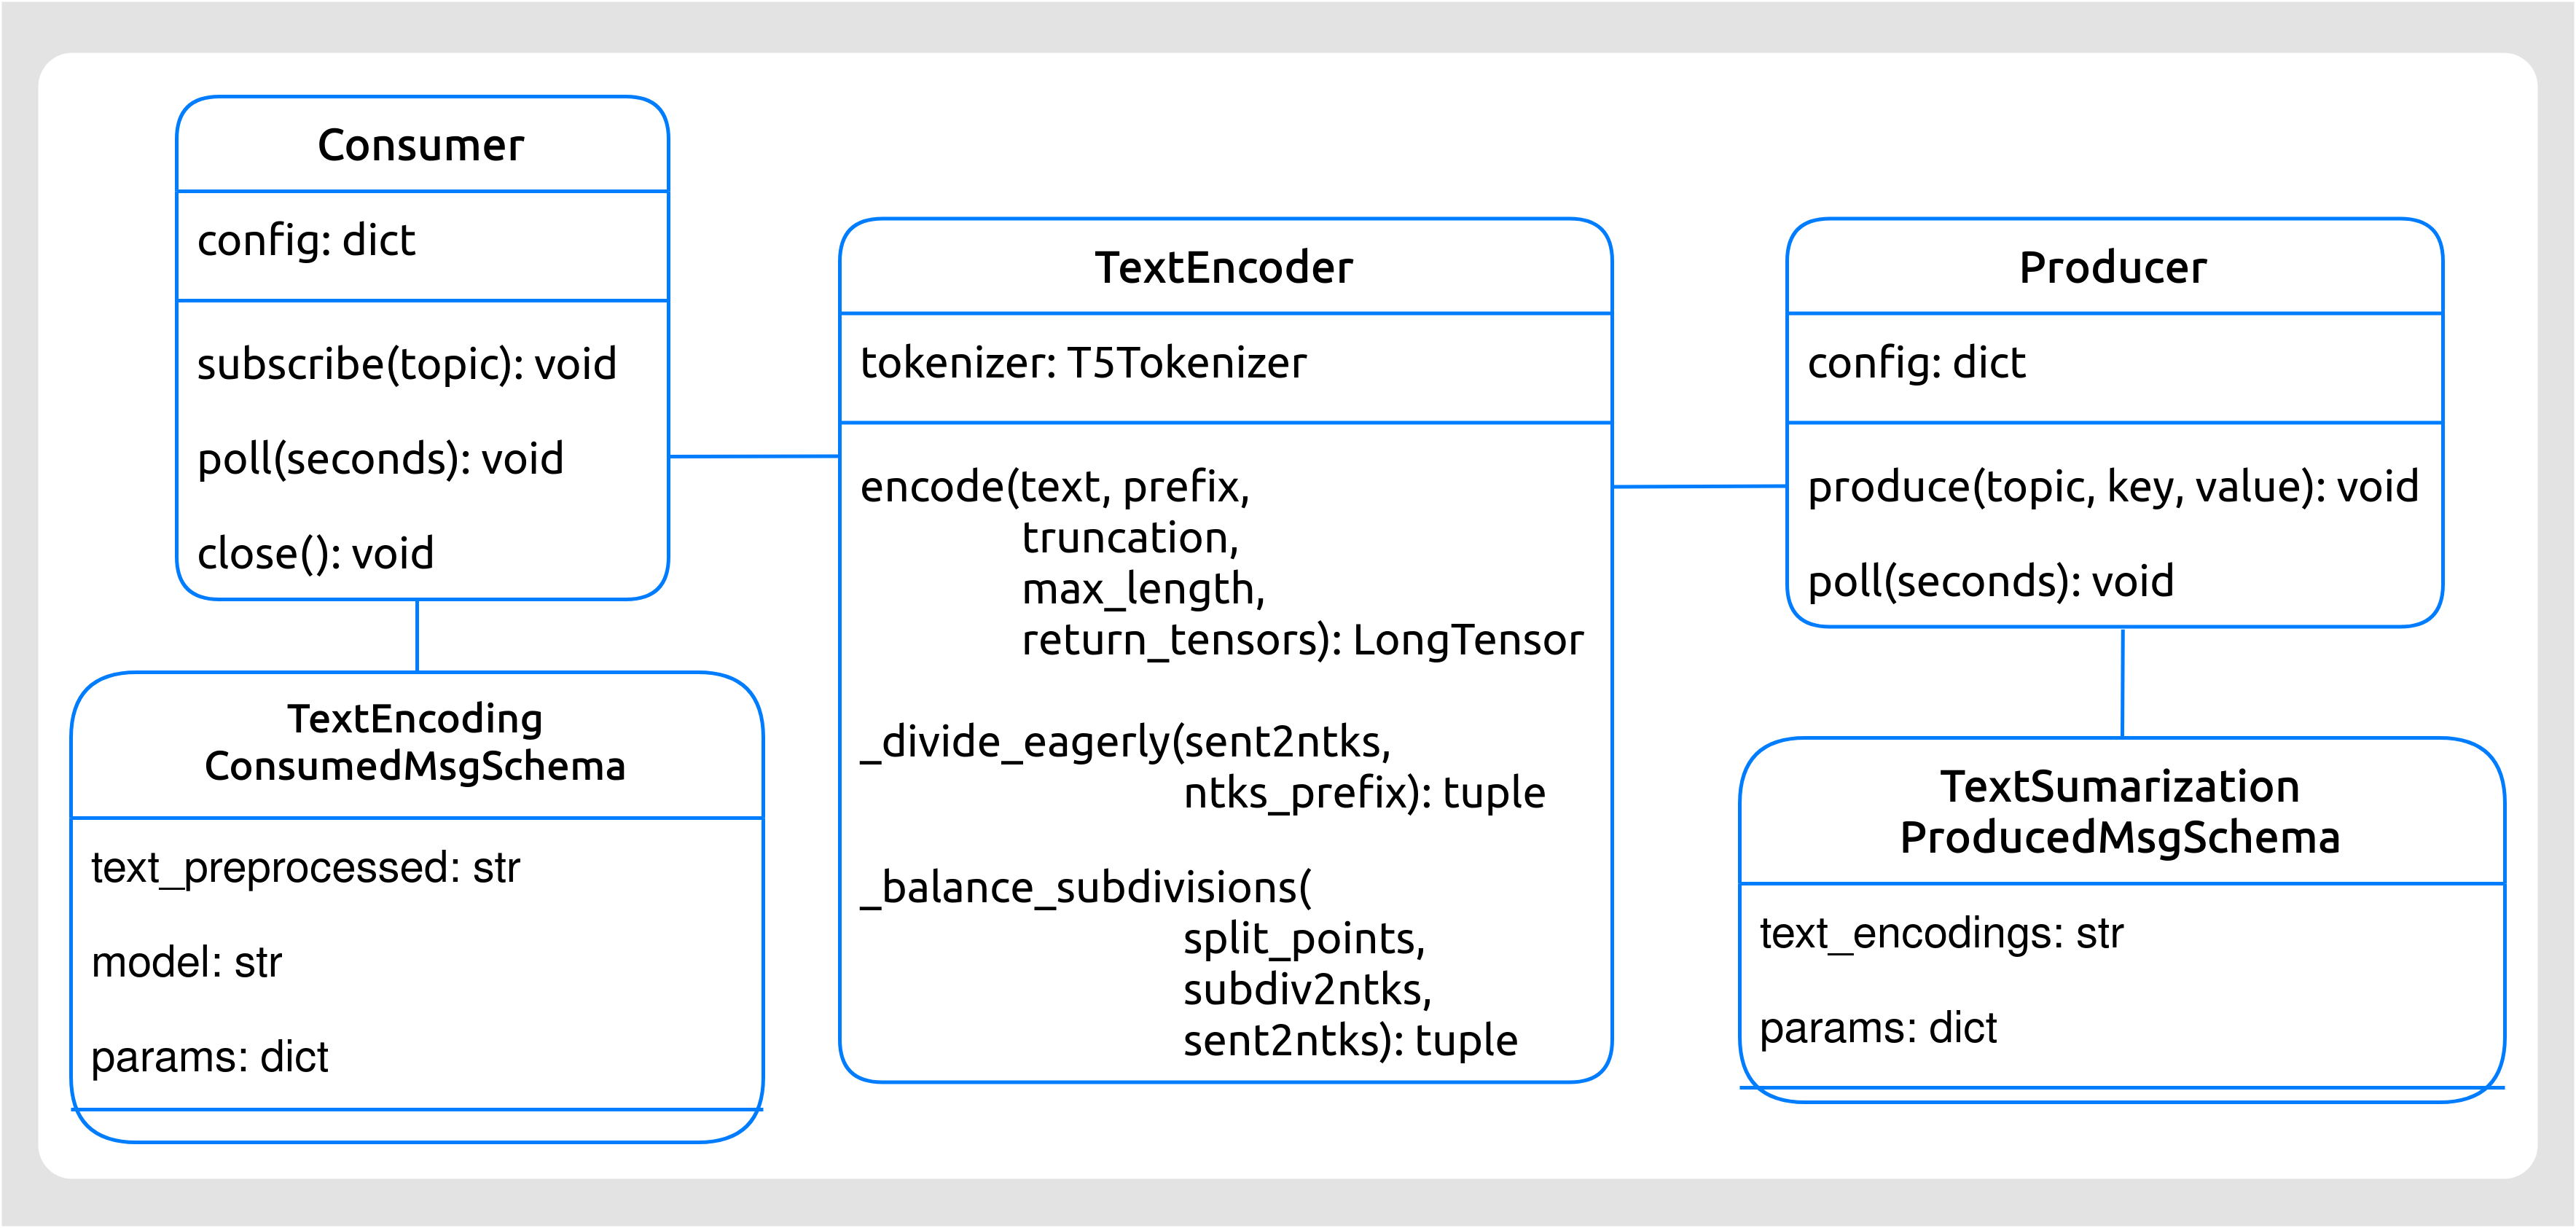
\includegraphics[width=\textwidth]{classes-encoder}
	\vspace{-0.5cm}
	\caption{Diagrama de clases del Codificador de textos.}
\end{figure}


\noindent
\textbf{\large Microservicio Generador de resúmenes}

Este microservicio se encarga de generar resúmenes a partir del texto codificado que recibe del Codificador.

Las clases del Generador de resúmenes son:

\vspace{-0.2cm}
\begin{itemize} [\textbullet]
	\item \textbf{Generador de resúmenes (\emph{Summarizer})}: esta clase es la encargada de generar los resúmenes.
	
	\item \textbf{Esquema para Mensajes Consumidos \\ (\emph{TextSummarizationConsumedMsgSchema})}: estructura (campos) que presenta un mensaje consumido por el Generador de resúmenes. Estos mensajes procederán del microservicio Codificador de textos.
	
	\item \textbf{Esquema para Mensajes Producidos \\ (\emph{TextPostprocessingProducedMsgSchema})}: estructura (campos) que presenta un mensaje producido al \emph{topic} del siguiente microservicio (el Post-procesador de textos).
\end{itemize}

\noindent
\textbf{Diagrama de clases}

\begin{figure}[h]
	\centering
	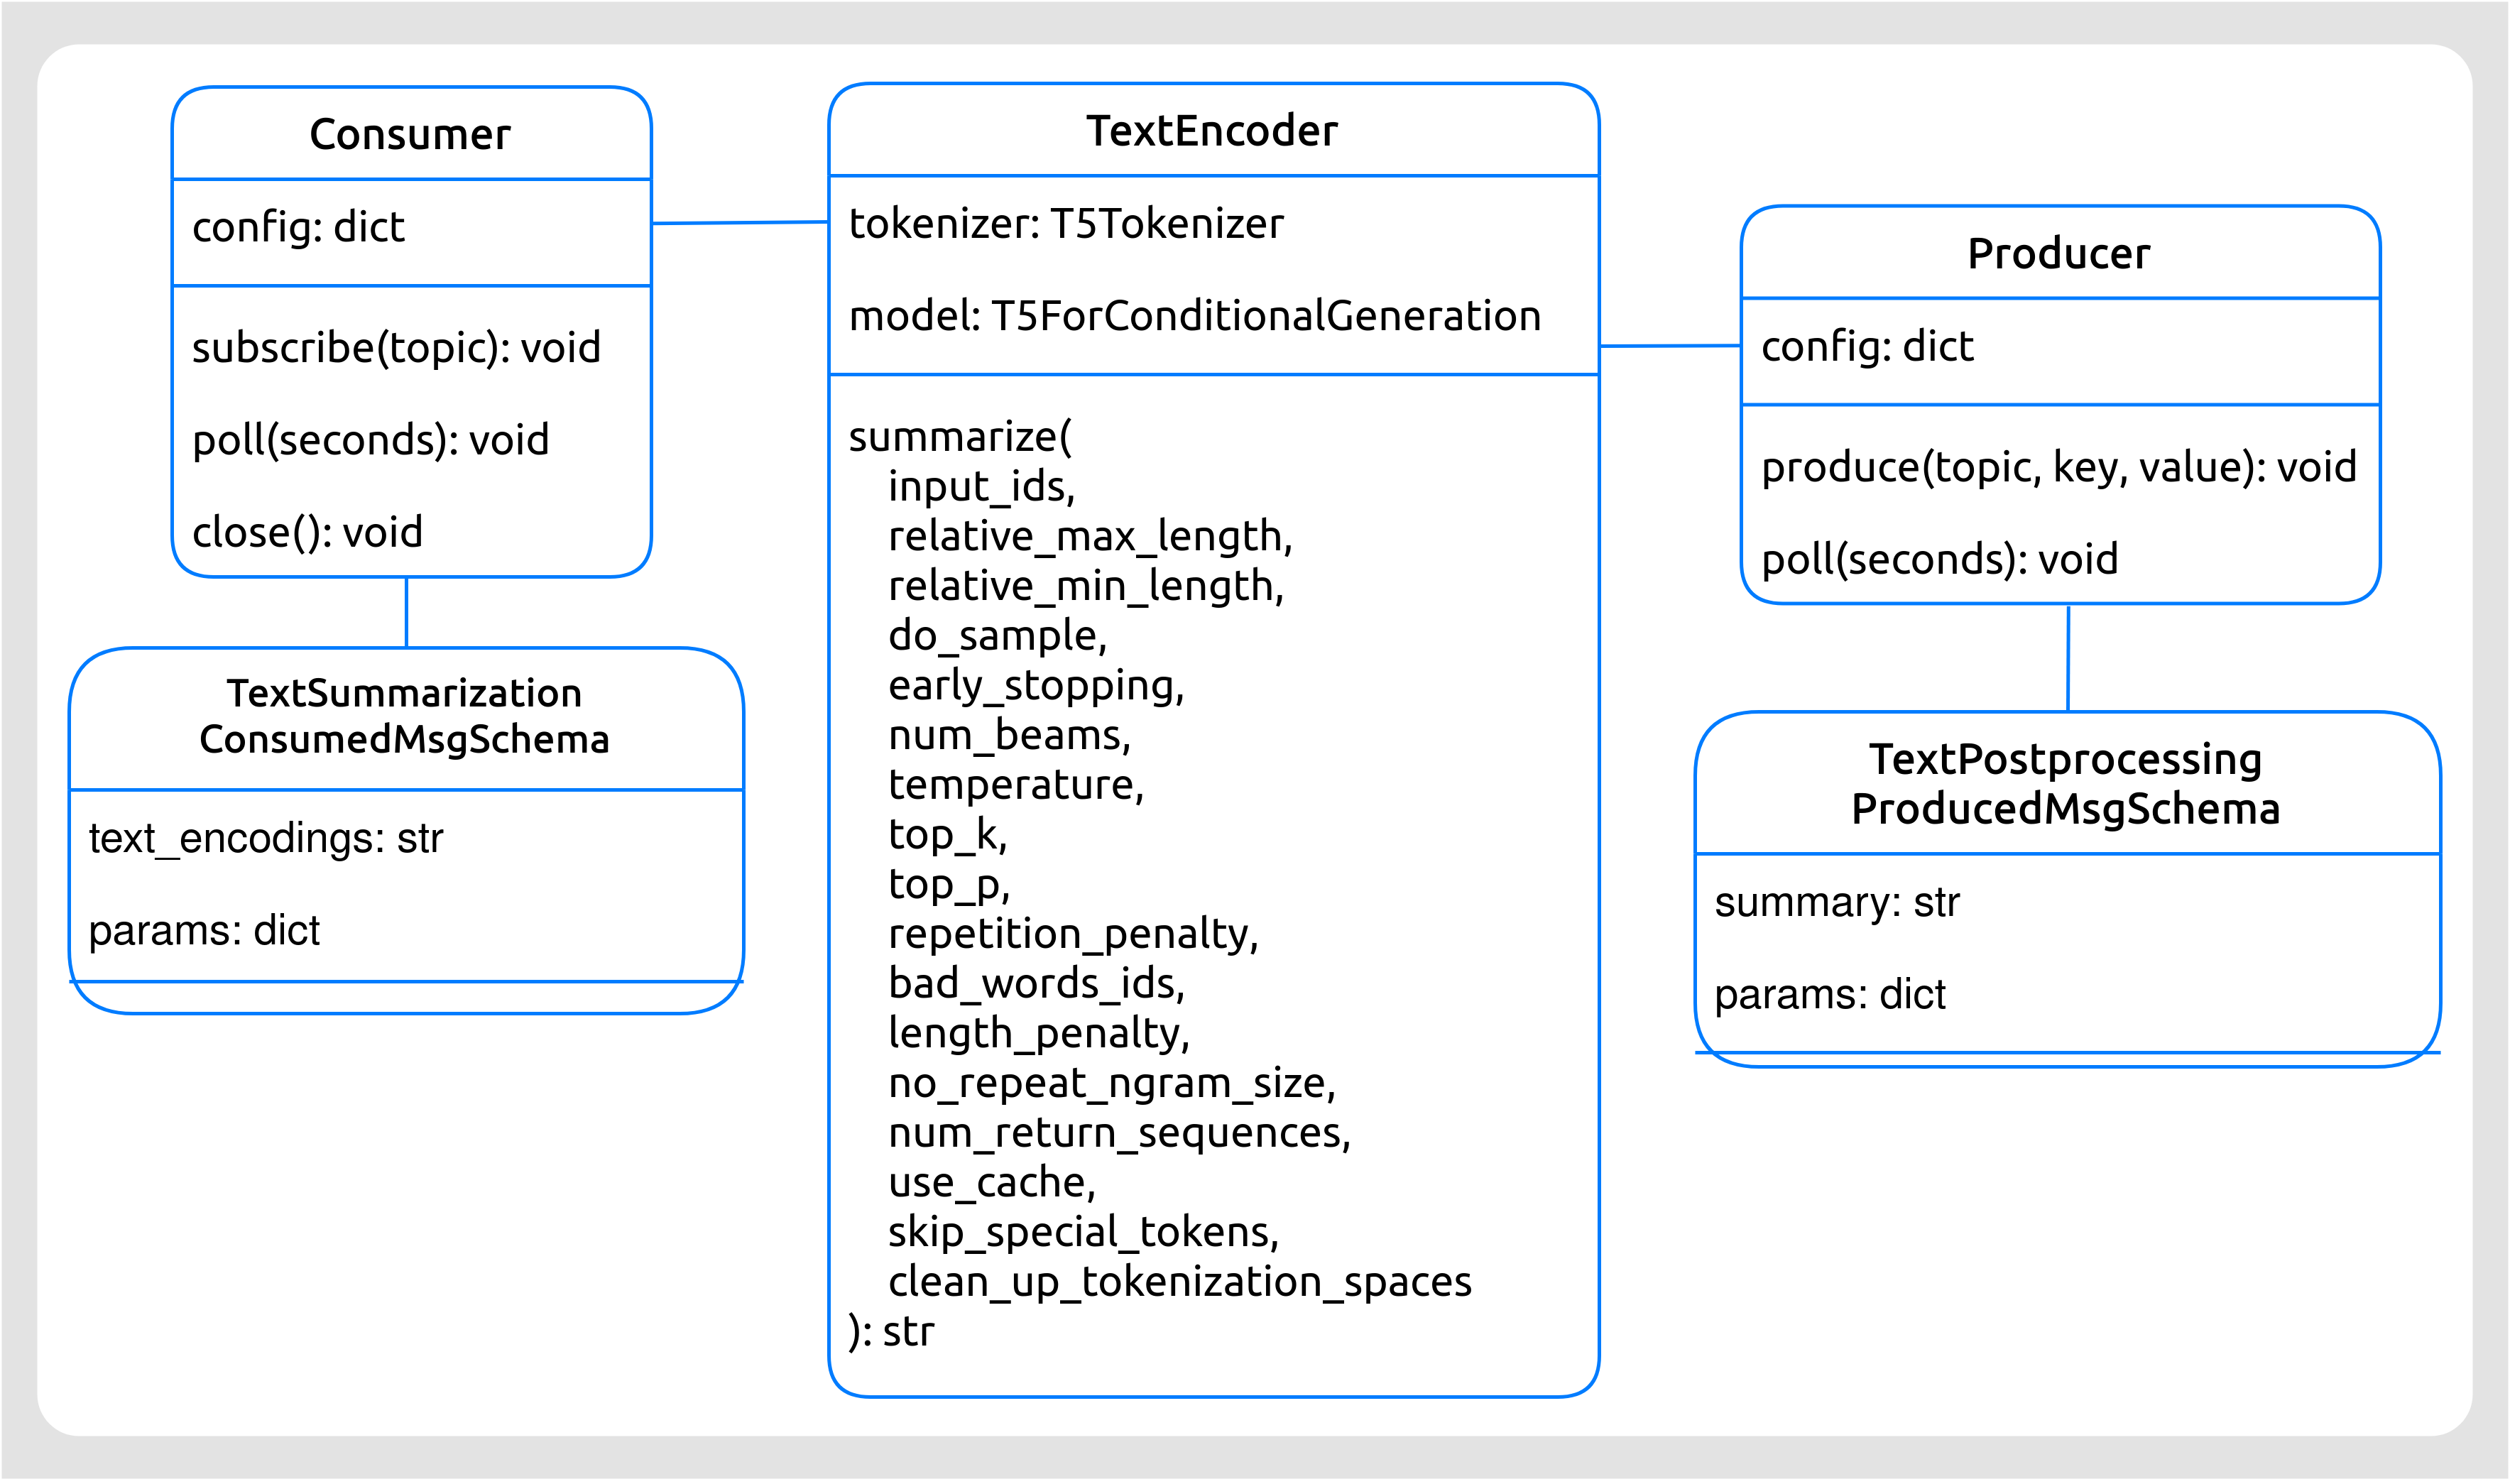
\includegraphics[width=\textwidth]{classes-summarizer}
	\vspace{-0.5cm}
	\caption{Diagrama de clases del Generador de resúmenes.}
\end{figure}



\noindent
\textbf{\large Microservicio Post-procesador de textos}

Este microservicio lleva a cabo el post-procesado del resumen entregado por el Generador de resúmenes.

El Post-procesador de textos tiene las siguientes clases.

\vspace{-0.2cm}
\begin{itemize} [\textbullet]
	\item \textbf{Post-procesador de textos (\emph{TextPostprocessor})}: esta clase es la encargada de post-procesar el texto.
	
	\item \textbf{Esquema para Mensajes Consumidos \\ (\emph{TextPostprocessingConsumedMsgSchema})}: estructura (campos) que presenta un mensaje consumido por el Post-procesador de textos. Estos mensajes procederán del microservicio Generador de resúmenes.
	
	\item \textbf{Esquema para Mensajes Producidos \\ (\emph{ReadyProducedMsgSchema})}: estructura (campos) que presenta un mensaje producido al siguiente \emph{topic}, \emph{Ready}.
\end{itemize}

\noindent
\textbf{Diagrama de clases}

\begin{figure}[h]
	\centering
	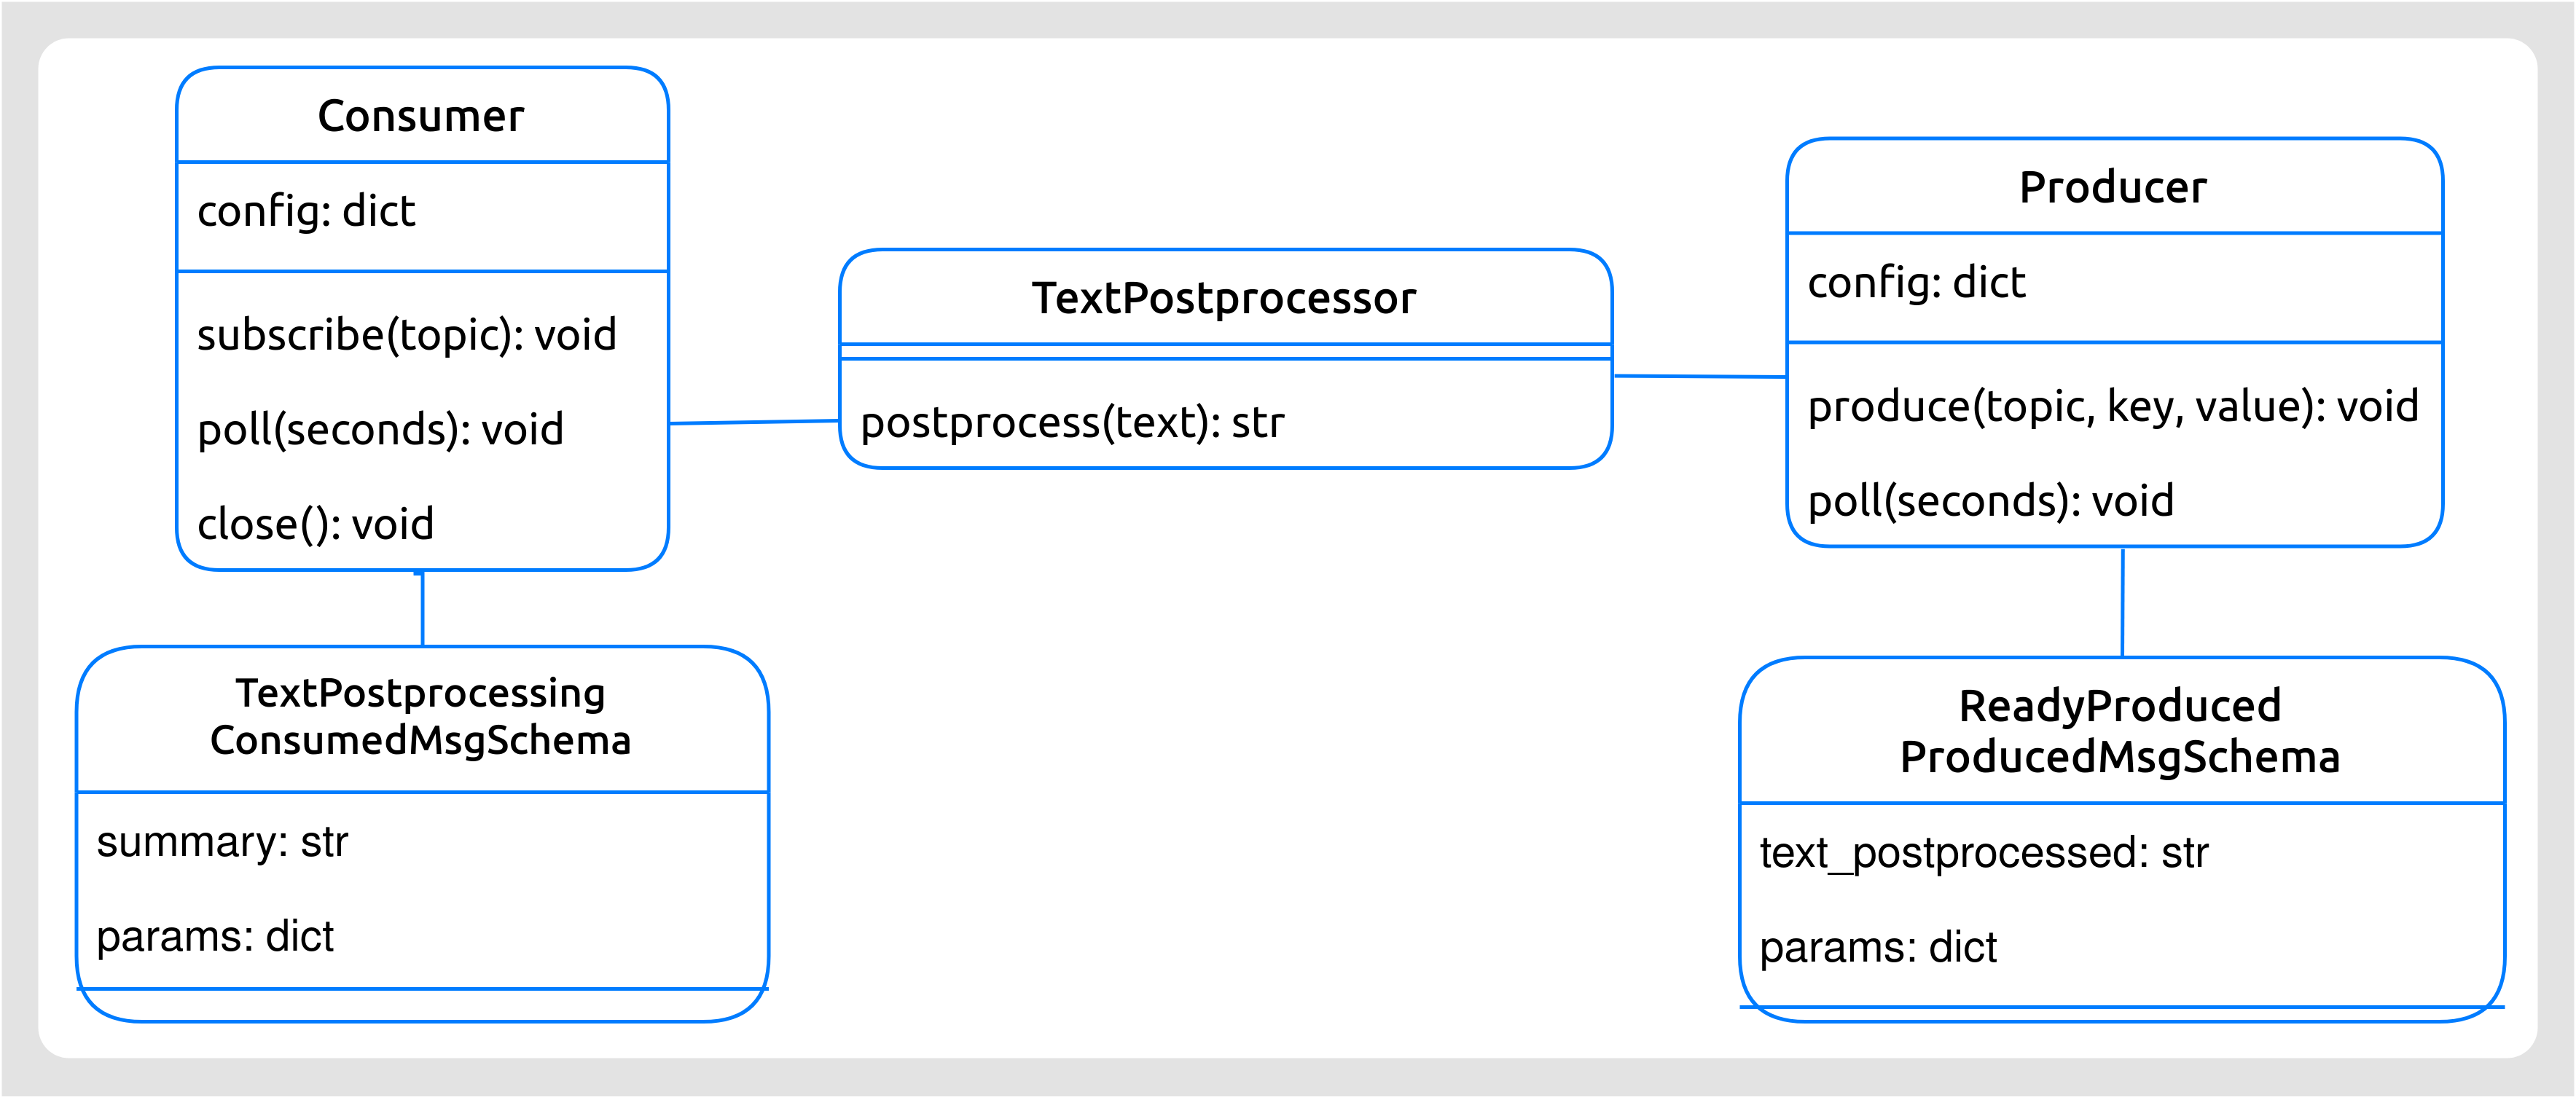
\includegraphics[width=\textwidth]{classes-postprocessor}
	\vspace{-0.5cm}
	\caption{Diagrama de clases del Post-procesador de textos.}
\end{figure}


\subsubsection{\Large \emph{Frontend}}

El \emph{frontend} está compuesto por la aplicación multiplataforma desarrollada siguiendo los patrones de \emph{Clean Architectura} y Diseño guiado por el dominio \emph{Domain Driven Design}. Para conocer los detalles concretos de la implementación de la arquitectura de la \emph{app}, se recomienda acudir a la sección ``Motivación tras las arquitecturas desarrolladas'' del capítulo ``Aspectos relevantes'' de la Memoria.

Las clases identificadas en la aplicación son las siguientes:

\vspace{-0.2cm}
\begin{itemize} [\textbullet]
	\item \textbf{JiztApp}: esta clase representa la aplicación en su conjunto. En el \texttt{main} de la aplicación, se ejecuta una instancia de esta clase.
	
	\item \textbf{NewSummaryPage}: se corresponde con la pantalla desde la cual los usuarios pueden solicitar nuevos resúmenes.
	
	\item \textbf{SummaryPage}: se corresponde con la pantalla en la que se muestra el resumen generado.
	
	\item \textbf{NewSummaryCubit}: clase encargada de transformar los eventos procedentes de los usuarios en la pantalla \texttt{NewSummaryPage} (por ejemplo, un \emph{click}), en acciones particulares de la aplicación.
	
	\item \textbf{SummaryCubit}: análoga a la anterior solo que en este caso para la pantalla \texttt{SummaryPage}.
	
	\item \textbf{JiztRepository}: clase que encapsula y centraliza la lógica de acceso a las fuentes de datos.
	
	\item \textbf{JiztCacheClient}: clase que gestiona el acceso a la base de datos local.
	
	\item \textbf{JiztApiClient}: clase que gestiona la comunicación con la REST API de JIZT.
	
	\item \textbf{Summary}: representa un resumen. En realidad, disponemos de tres representaciones de un resumen, cada una correspondiéndose con cada uno de los dominios (capa de dominio, caché y REST API). No obstante, la estructura de las mismas es análoga; por consiguiente, las sintetizamos todas en una única clase para simplificar el esquema de diseño.
\end{itemize}


\begin{figure}[h]
	\centering
	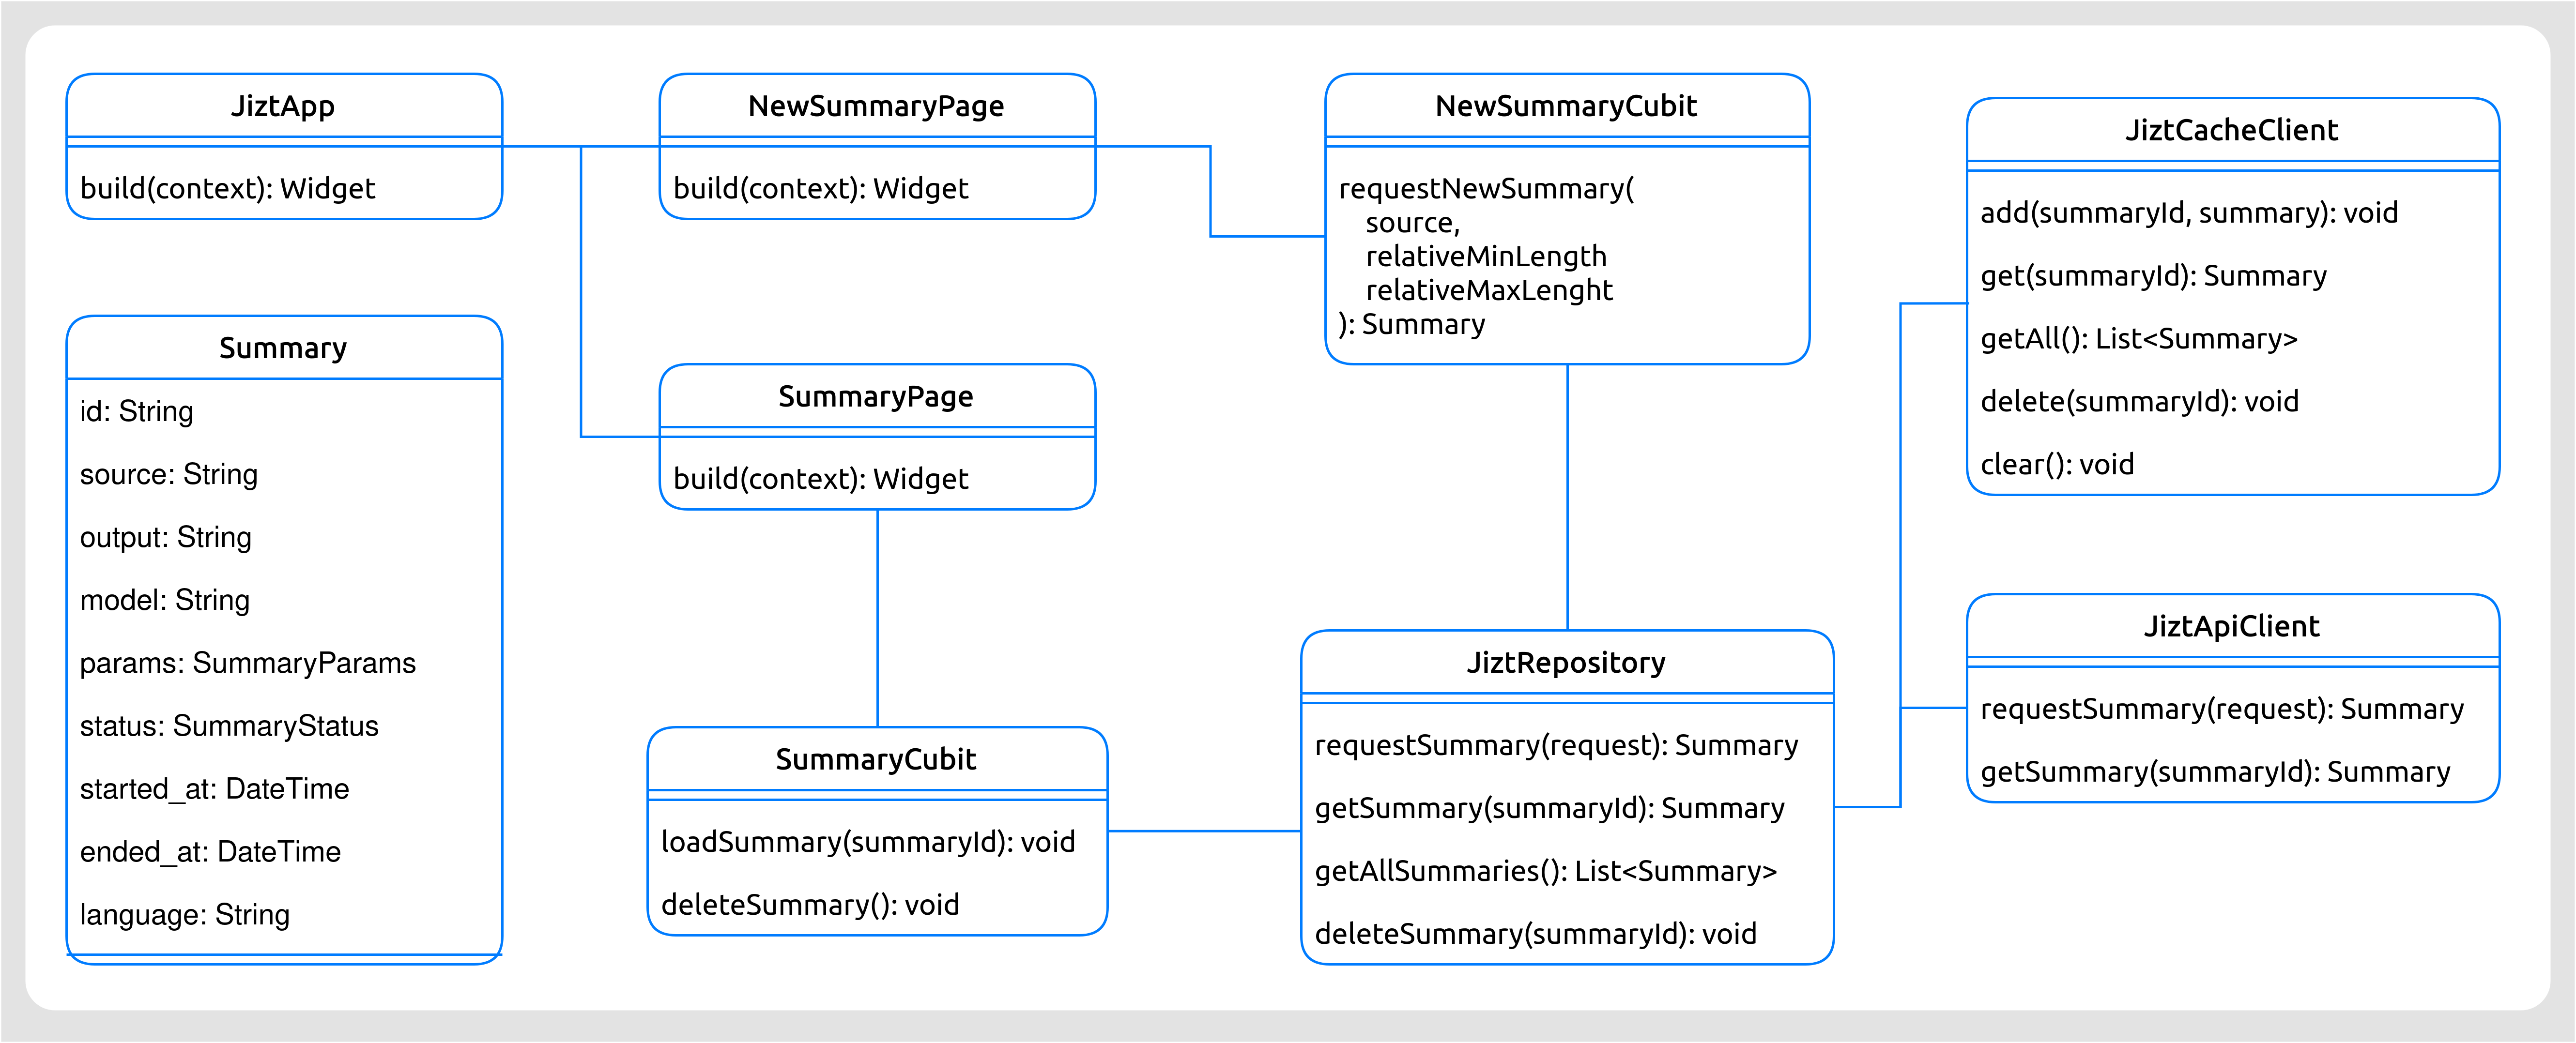
\includegraphics[width=\textwidth]{classes-app}
	\vspace{-0.5cm}
	\caption{Diagrama de clases de la aplicación de JIZT.}
\end{figure}


\section{Diseño procedimental}

En esta sección repasamos una vez más los pasos que se llevan a cabo tanto en el \emph{backend} a la hora de atender las peticiones de los clientes y generar los resúmenes, como en la aplicación, encargada de gestionar los resúmenes de los usuarios.

En la sección correspondiente al \emph{backend} del capítulo ``Técnicas y Herramientas'', explicábamos cómo se gestionaba la comunicación entre los clientes y la REST API a través de peticiones HTTP. Recordemos el proceso:

\begin{enumerate}
	\item El cliente realiza una petición HTTP POST, incluyendo en el cuerpo el texto a resumir, así como los parámetros del resumen a generar.
	
	\item Ingress (API \emph{Gateway}) comprueba que dicha petición se está haciendo a un \emph{endpoint} válido, y en ese caso la redirige hacia el \emph{Dispatcher}.
	
	\item El \emph{Dispatcher} realiza una serie de comprobaciones:
	\begin{enumerate}	
		\item Se consulta en la base de datos si ya existe un resumen generado para ese texto con esos parámetros. En ese caso, se responde al cliente con los datos del resumen (\texttt{output}, \texttt{source}, \texttt{started\_at}, \texttt{ended\_at}, etc.).
		
		\item En caso contrario, se responde con el mismo esquema de datos, solo que el \texttt{output} será \texttt{null}. Al mismo tiempo, se produce un mensaje al \emph{topic} del pre-procesador de textos, conteniendo el texto y los parámetros del resumen, comenzando el proceso de generación.
	\end{enumerate}
	
	\item El pre-procesador está constantemente comprobando si existen mensajes nuevos en su \emph{topic}. En ese caso los consume, realiza las tareas de pre-procesado, y produce el resultado en el \emph{topic} del codificador.
	
	\item Este proceso continua de forma análoga hasta llegar al post-procesador, el cual produce el resumen final al \emph{topic} <<Listo>> (\emph{Ready}). El \emph{Dispatcher}, en ese momento, consume el mensaje, y actualiza la base de datos.
	
	\item Mientras el proceso de resumen se completa, el cliente realiza peticiones GET de manera periódica, hasta que la API REST finalmente responde con el resumen generado.
\end{enumerate}

La \autoref{seq-app} ilustra este proceso de forma gráfica, a través de un diagrama de secuencia.

A su vez, en la aplicación, es decir, el \emph{frontend}, de llevan a cabo los siguientes pasos:

\begin{enumerate}
	\item El usuario solicita generar un nuevo resumen, pulsando para ello sobre la pantalla.
	
	\item El evento se transforma a través del \emph{cubit} en un petición de resumen al repositorio.
	
	\item El repositorio realiza una petición HTTP POST al \emph{backend} para obtener el \emph{id} del resumen a partir del texto fuente, los parámetros del resumen, y el modelo.
	
	\item Una vez obtenido el \emph{id} del resumen, se consulta la base de datos local (capa de caché) para conocer si ya se dispone localmente del resumen solicitado. En ese caso, se devuelve el resumen, y se actualiza la pantalla para mostrárselo al usuario.
	
	\item En caso contario, se realiza peticiones GET periódicas a la API REST hasta que el resumen se completa. Finalmente, se actualiza la pantalla.
\end{enumerate}

En la \autoref{seq-app}, se incluye un diagrama de clases que describe el proceso de manera más detallada.

\vspace{1cm}

\begin{figure}[h]
	\centering
	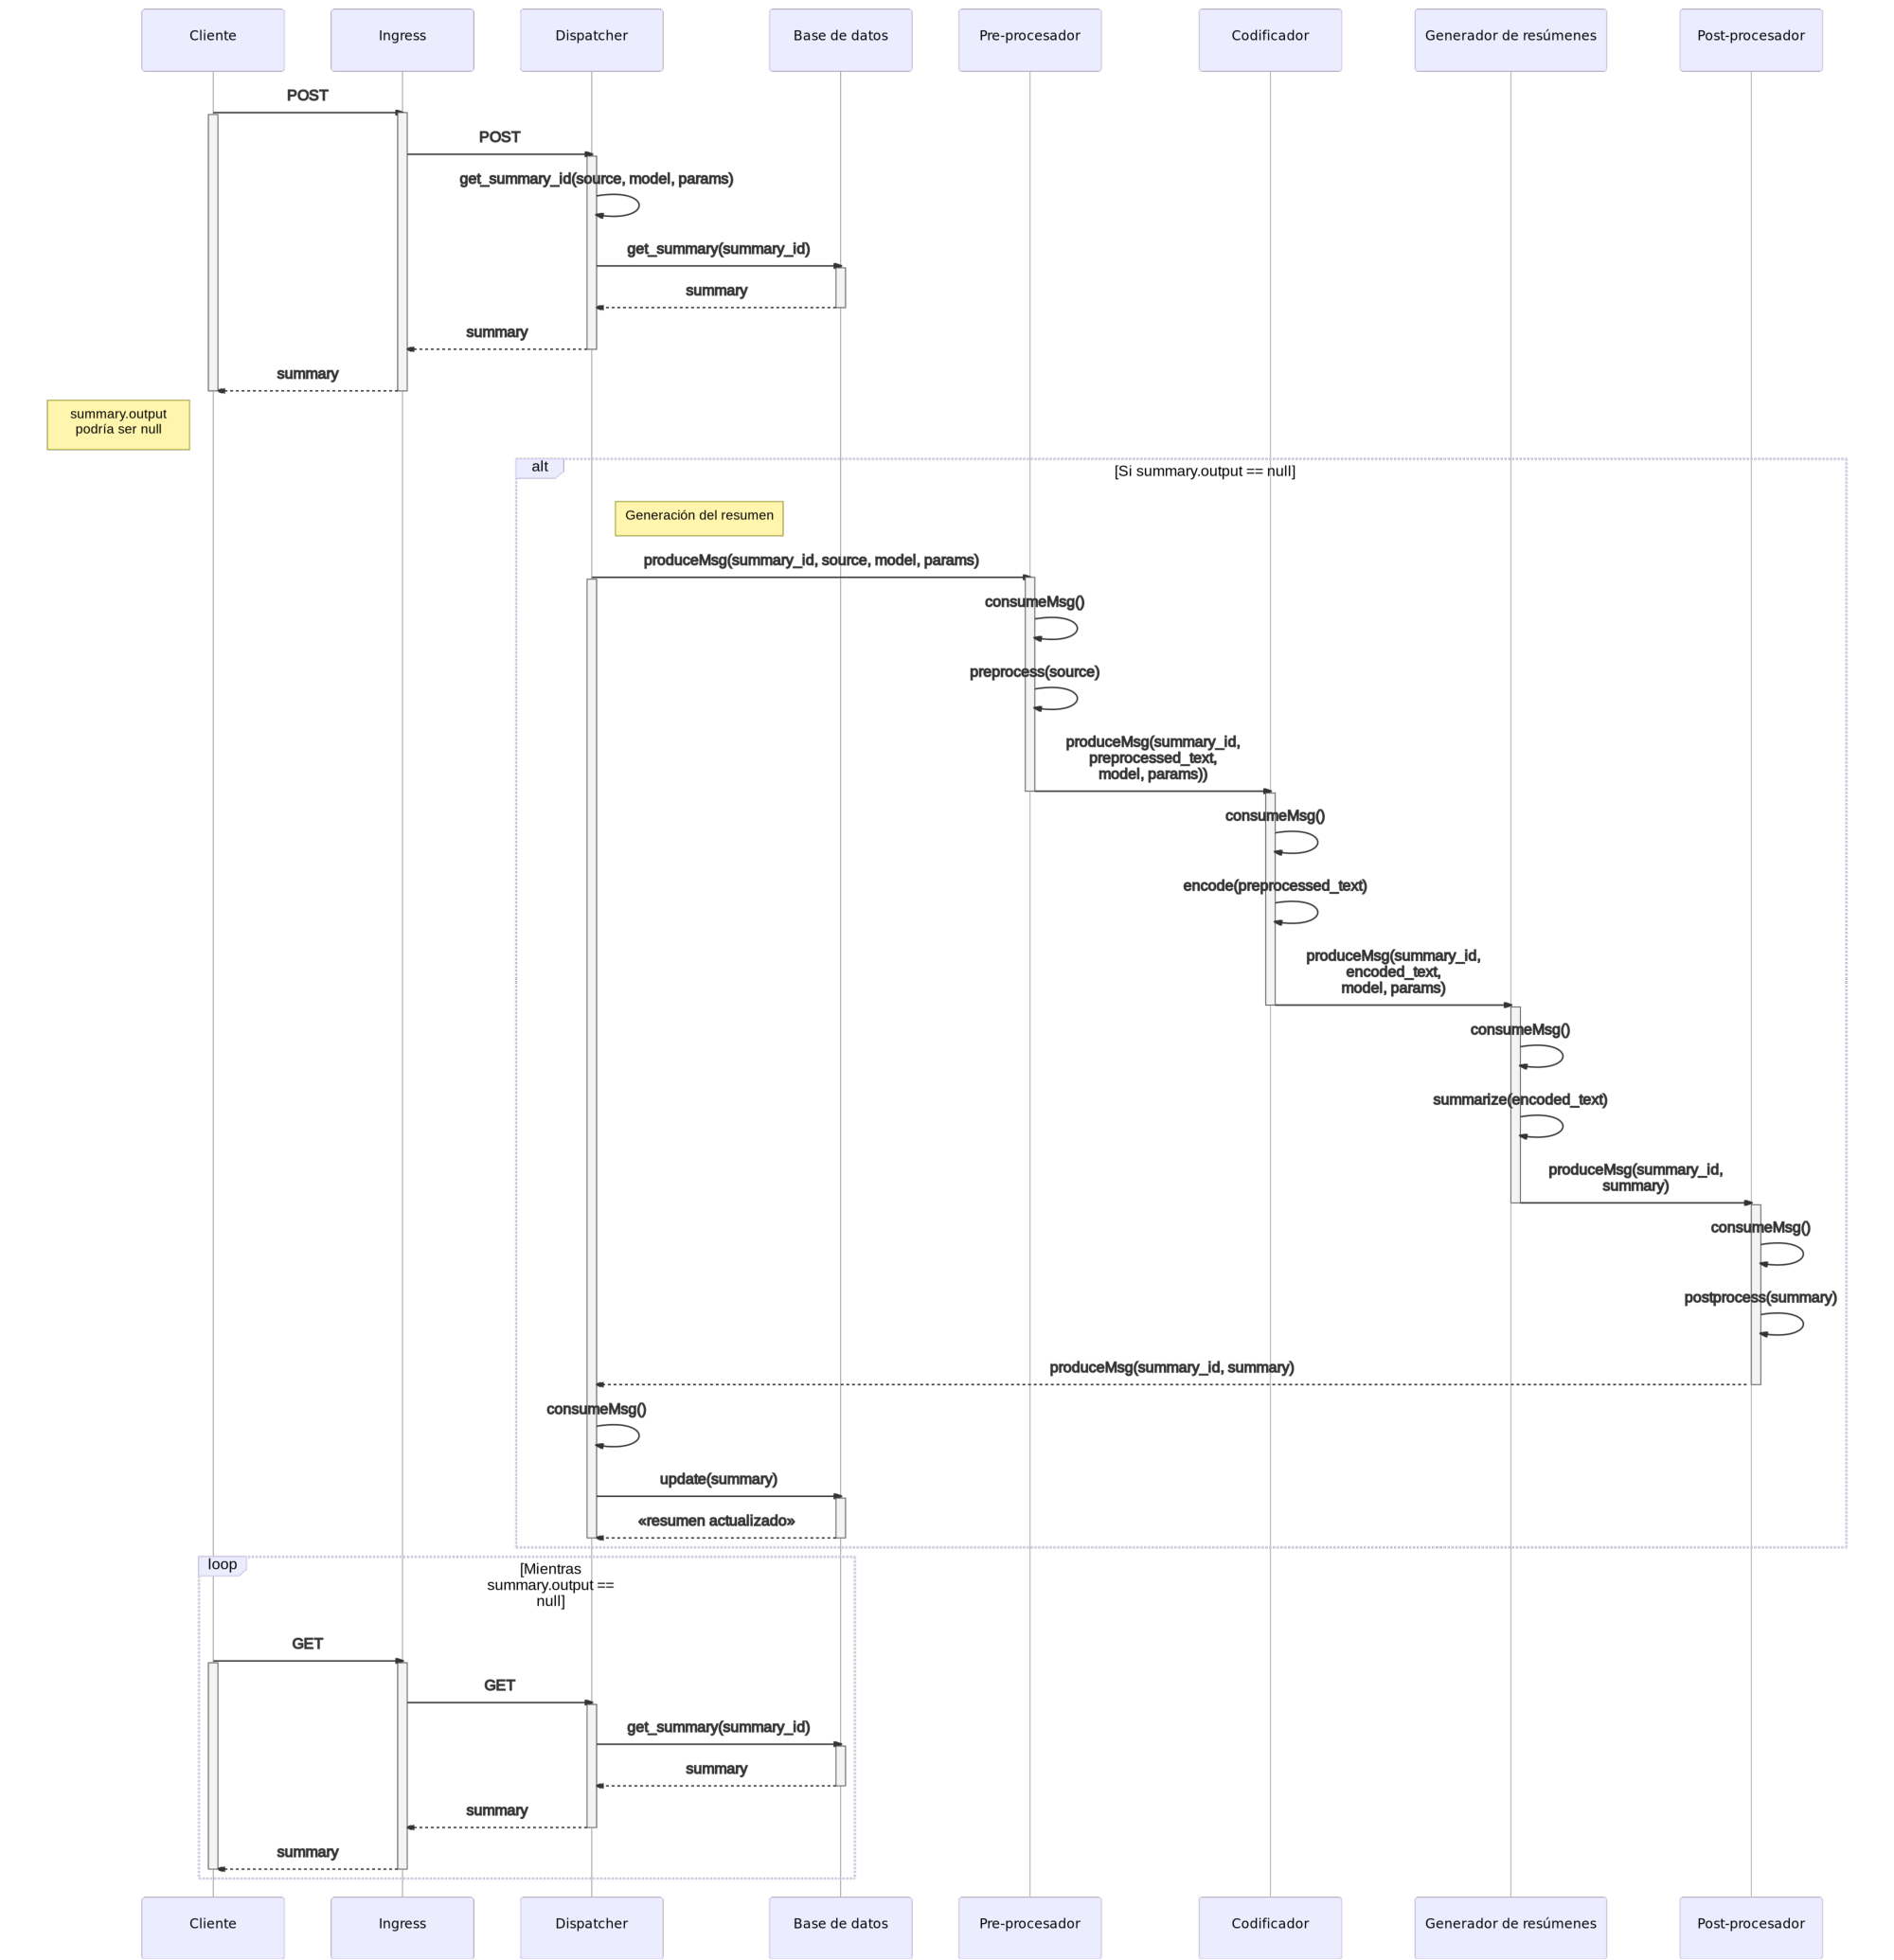
\includegraphics[width=\textwidth]{seq-diagram-api}
	\caption{Diagrama de secuencia del \emph{backend}.}
	\label{seq-api}
\end{figure}

\vspace*{1cm}

\begin{landscape}
	\begin{figure}[h]
		\centering
		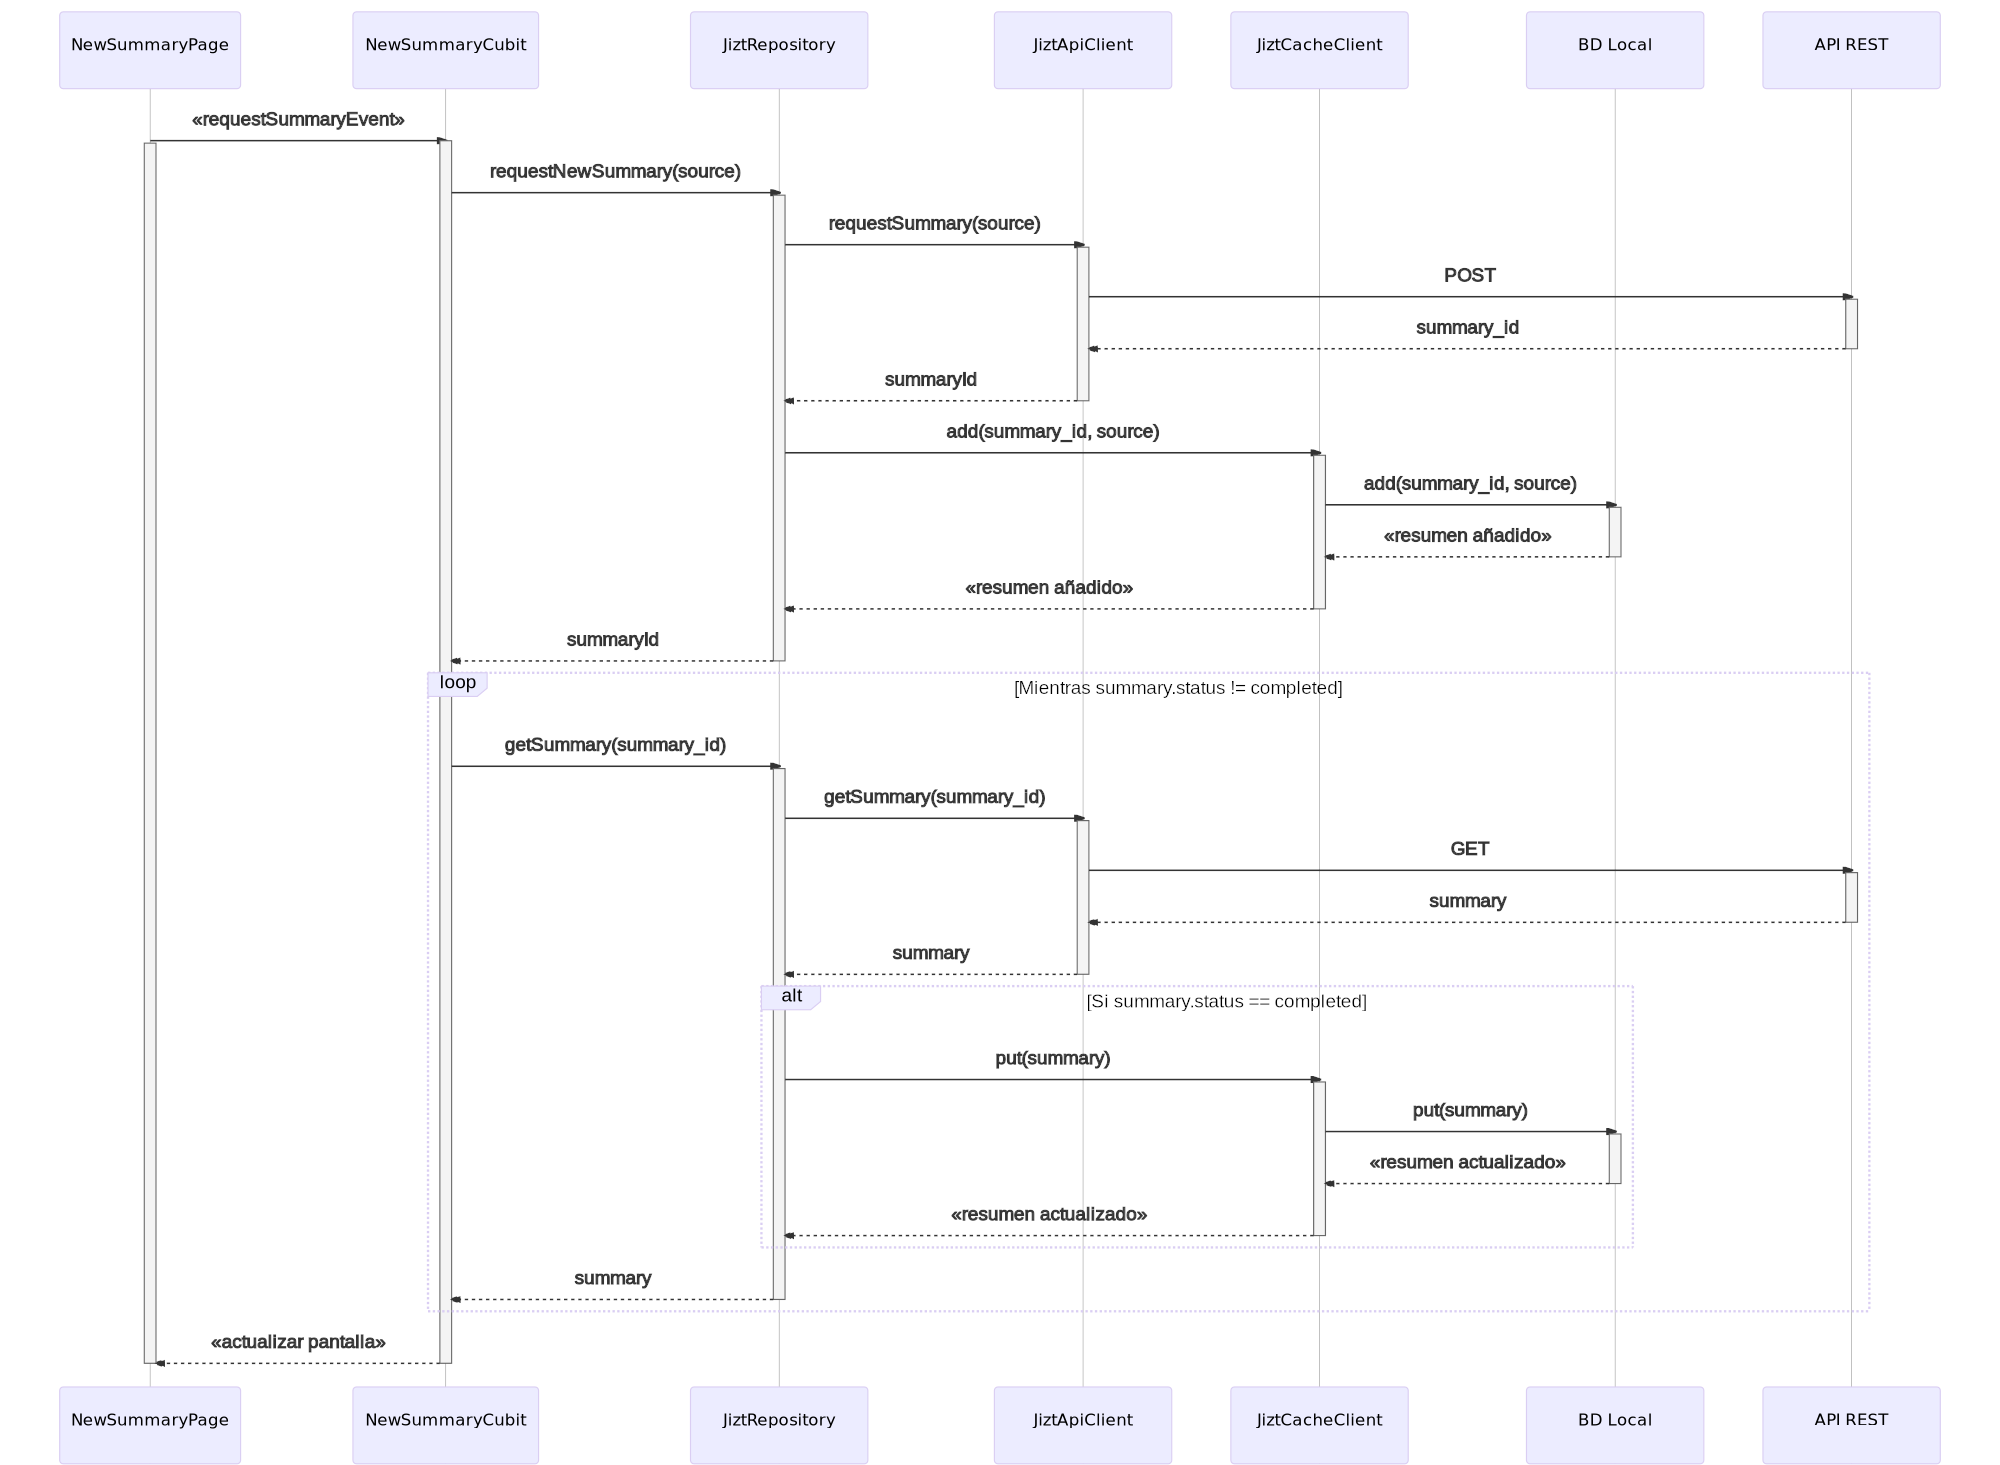
\includegraphics[width=1.3\textwidth]{seq-diagram-app}
		\caption{Diagrama de secuencia de la aplicación.}
		\label{seq-app}
	\end{figure}
\end{landscape}

\section{Diseño arquitectónico}

Dado que el diseño arquitectónico conforma uno de los principales aspectos a destacar de todo el proyecto, se ha incluido de manera detallada en la Memoria.

\subsubsection{\Large \emph{Backend}}

Por tanto, en esta sección llevaremos a cabo un resumen de los principales puntos de la arquitectura, e incluiremos información adicional acerca de los retos que surgieron, y cómo se resolvieron, dando con el diseño arquitectónico final.

Como se indica en la Memoria, para el \emph{backend} se ha desarrollado una \textbf{arquitectura de microservicios}, a través de la cual podemos separar cada paso en la generación de resúmenes (pre-procesado, codificación, generación del resumen, post-procesado0), en módulos independientes, favoreciendo los siguientes aspectos:

\vspace{-0.2cm}
\begin{itemize} [\textbullet]
	\item Gracias a la división en microservicios, conseguimos una gran flexibilidad; los cambios en uno de los pasos en la generación del resumen no influyen al resto.
	
	\item Facilita la detección y corrección de cuellos de botella en el proceso, dado que podemos monitorizar de forma precisa el rendimiento de cada microservicio.
	
	\item La arquitectura es fácilmente escalable tanto en términos de los microservicios ya existentes, aumentando el número de réplicas de cada microservicio (permitiendo la generación en paralelo de varios resúmenes), como en términos de la adicción de nuevos microservicios, por ejemplo, diferentes modelos para distintos idiomas.
	
	\item Asegura una alta disponibilidad, ya si uno de los microservicios falla, el sistema crea una nueva instancia y finaliza el microservicio defectuoso. Adicionalmente, con una arquitectura de microservicios eliminamos cualquier posible punto de único fallo (\emph{single point of failure}).
\end{itemize}

Otro de los principales aspectos de la arquitectura es cómo se lleva a cabo la comunicación y el correcto enrutado de los mensajes entre los diferentes microservicios. Al tratarse de un proceso secuencial, la salido de un microservicio será la entrada del siguiente.

Inicialmente, se pensó en resolver esta situación mediante el patrón de \emph{routing-slips} (hojas de ruta) \cite{routing-slip}. Con este patrón se incluye en el propio mensaje la ruta que este debe seguir, por lo que, implementando un \emph{router} en cada microservicio que interpretara la hoja de ruta, podríamos, resolver el problema del enrutado. En cuanto a cómo se llevaría a cabo la comunicación, esta se podría hacer mediante peticiones HTTP, de forma que cada microservicio implementara su propia REST API.

Siguiendo esta estrategia, junto con el patrón de API \emph{gateway}, a través que se ofrece un punto de entrada al \emph{backend}, el diseño de la arquitectura quedaba como se muestra en la \autoref{fig:deprecated-arch}.

Poco después, conocimos acerca de la \textbf{arquitectura dirigida por eventos} \cite{event-driven}, y de Kafka \cite{apache-kafka}, una de las herramientas más apropiadas y avanzadas a día de hoy para este tipo de arquitectura\footnote{\, De nuevo, referimos al lector a la Memoria, donde se recogen las principales ventajas, tanto de este patrón arquitectónico, como de Kafka.}.

Con este nuevo diseño, la arquitectura se simplificaba en gran medida, y problemas como el escalado, o la entrega fiable de mensajes, corrían a cargo de Kafka, quienes gestionaba estos y otros aspectos de manera automática.

La arquitectura final del \emph{backend} se ilustra en la \autoref{fig:final-arch-backend}.


\subsubsection{\Large \emph{Frontend}}

Gracias a la vibrante comunidad de Flutter \cite{flutter-es}, dar con la arquitectura más apropiada para la aplicación resultó un proceso más fluido.

Antes de comenzar este proyecto, habíamos oído del concepto de \emph{Clean Architecture} \cite{martin15}, aunque no habíamos indagado muy en profundidad en sus proposiciones. No obstante, en nuestra formación de Flutter, apareció de nuevo, e incluso supimos que existe un paquete para Flutter que simplifica la implementación de este patrón \cite{flutter-clean-arch}.

A continuación, nos informamos sobre el patrón BLoC \cite{bloc-pattern}, muy popular también dentro de la comunidad Flutter. Por suerte, también existe un paquete para la implementación de este patrón \cite{bloc-package}.

Finalmente, la arquitectura quedó como se muestra en la \autoref{fig:final-arch-app}.

La información completa acerca de la arquitectura de la aplicación se encuentra, asimismo, en la Memoria.

\newpage

\vspace*{2cm}

\begin{figure}[h!]
	\centering
	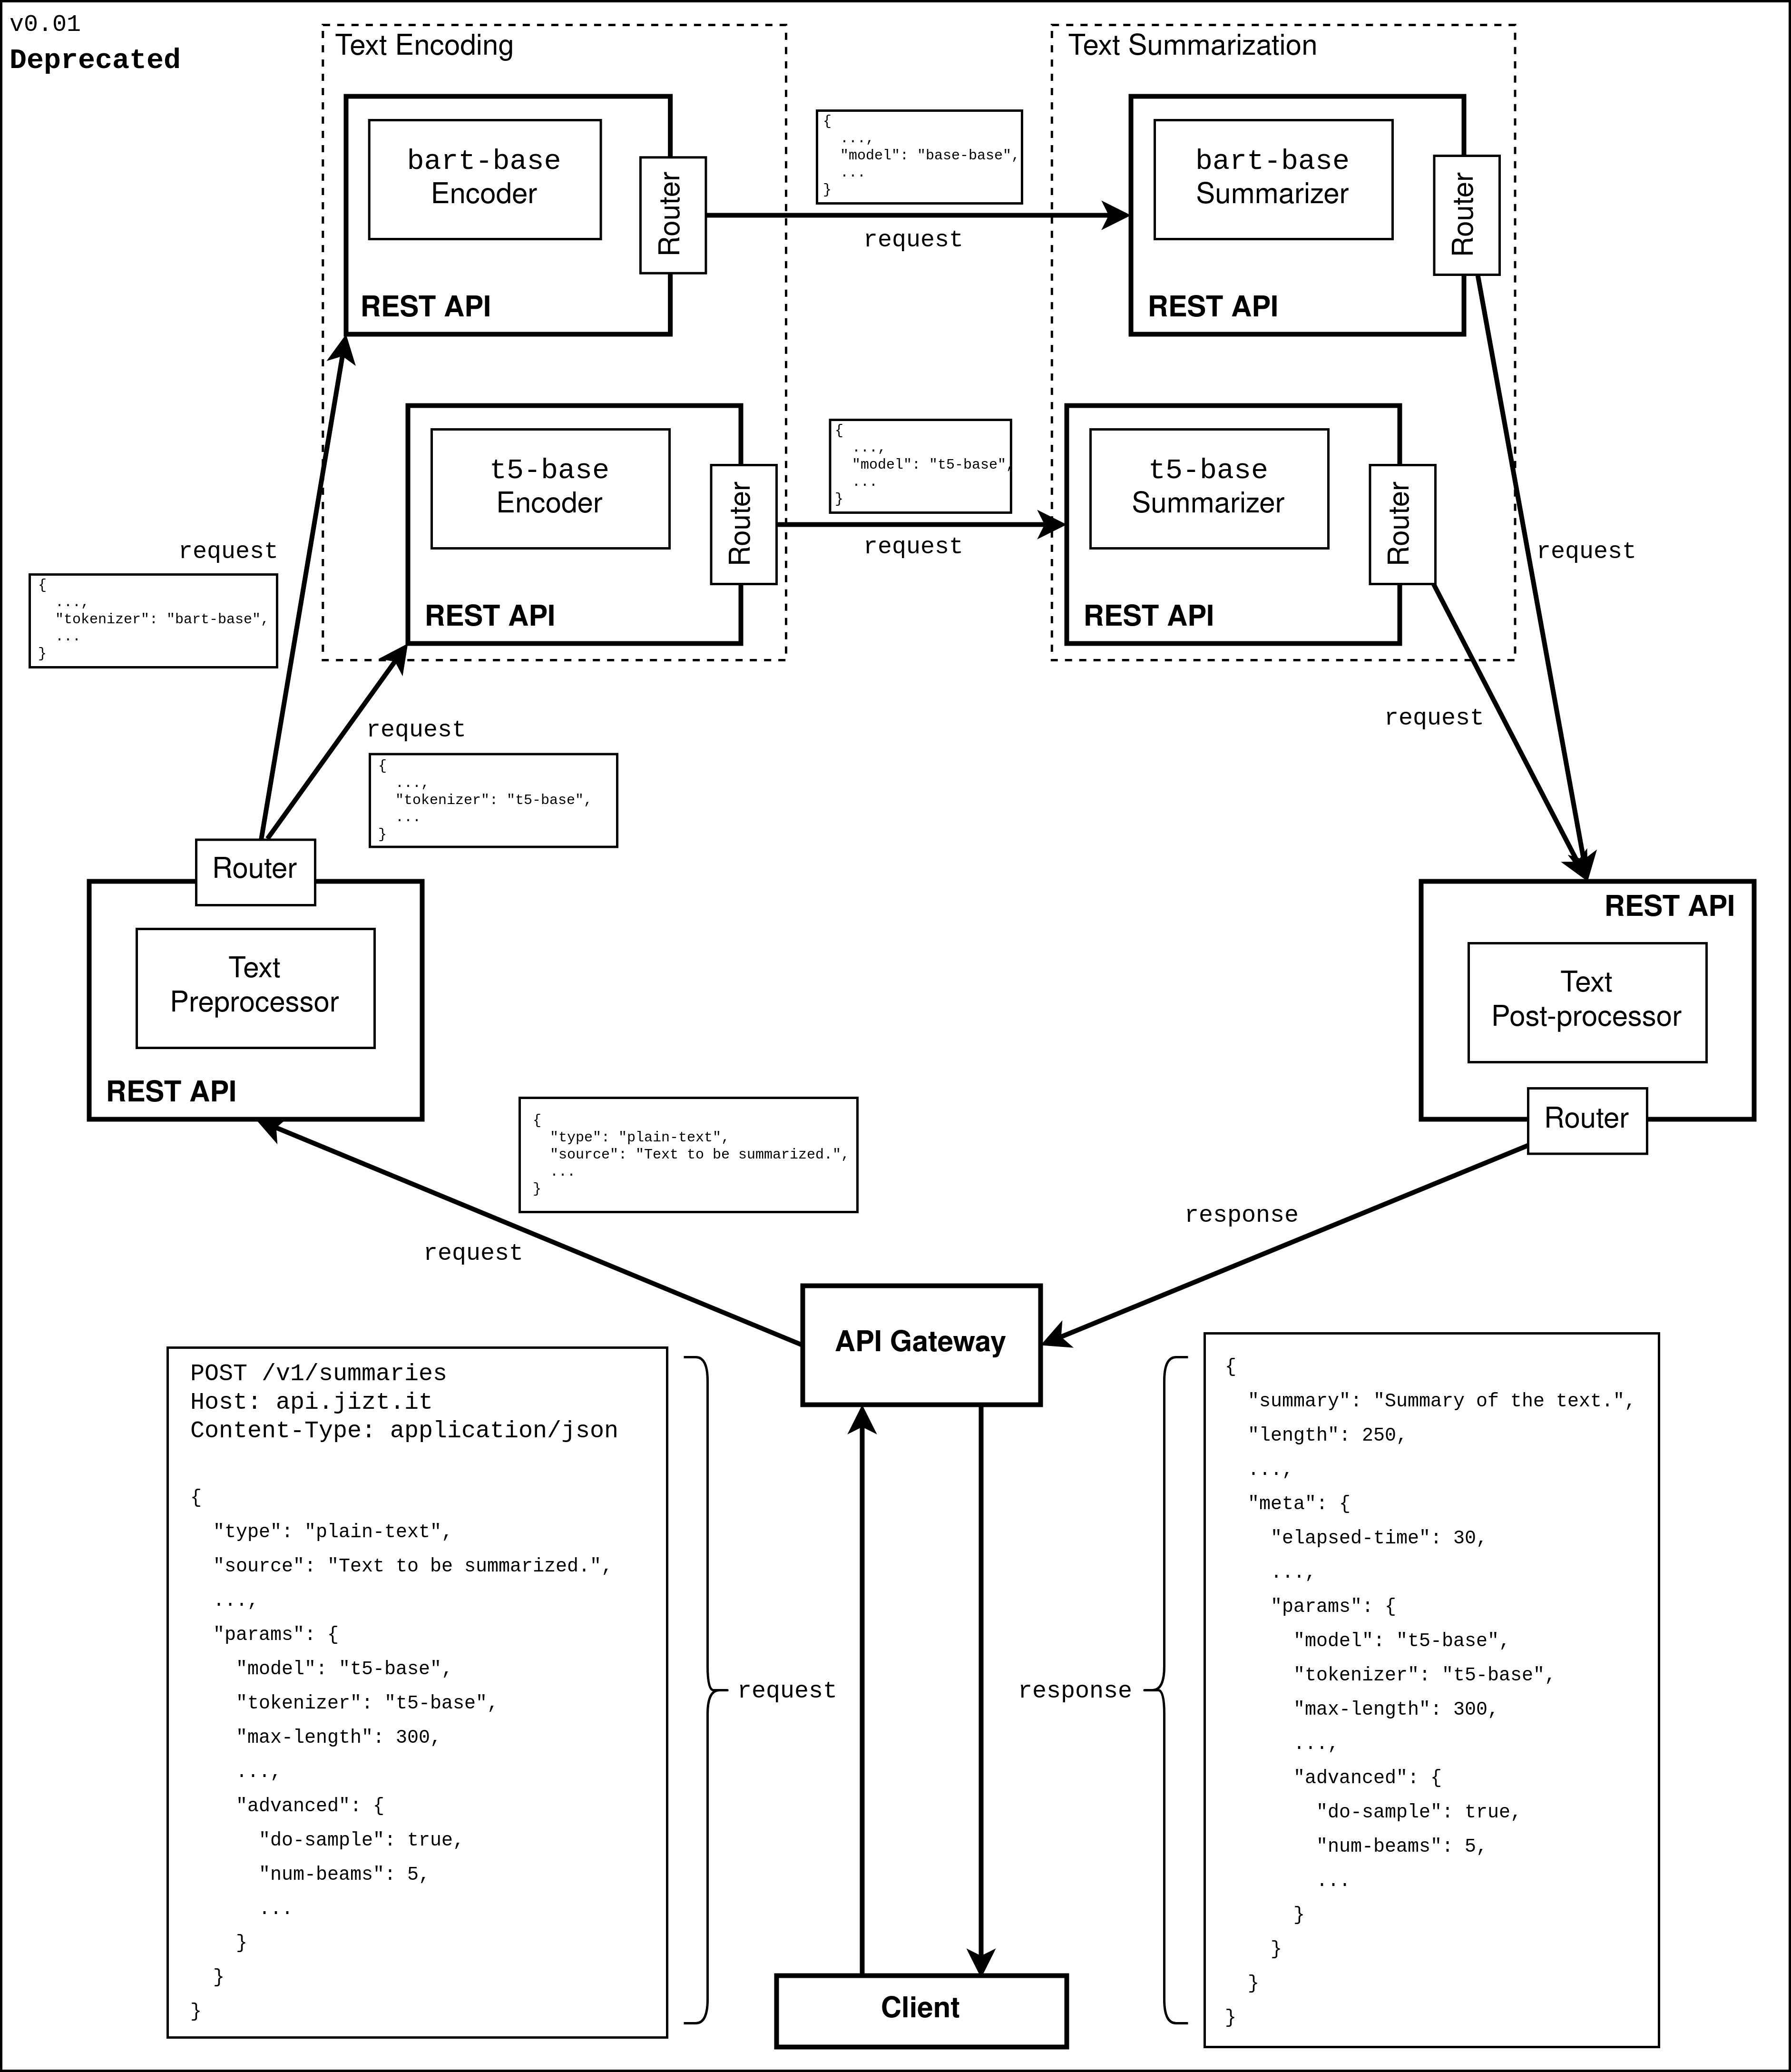
\includegraphics[width=\textwidth]{deprecated-arch}
	\vspace{-0.5cm}
	\caption{Primera aproximación para el diseño arquitectónico del \emph{backend}.}
	\label{fig:deprecated-arch}
\end{figure}

\newpage

\vspace*{2cm}

\begin{figure}[h!]
	\centering
	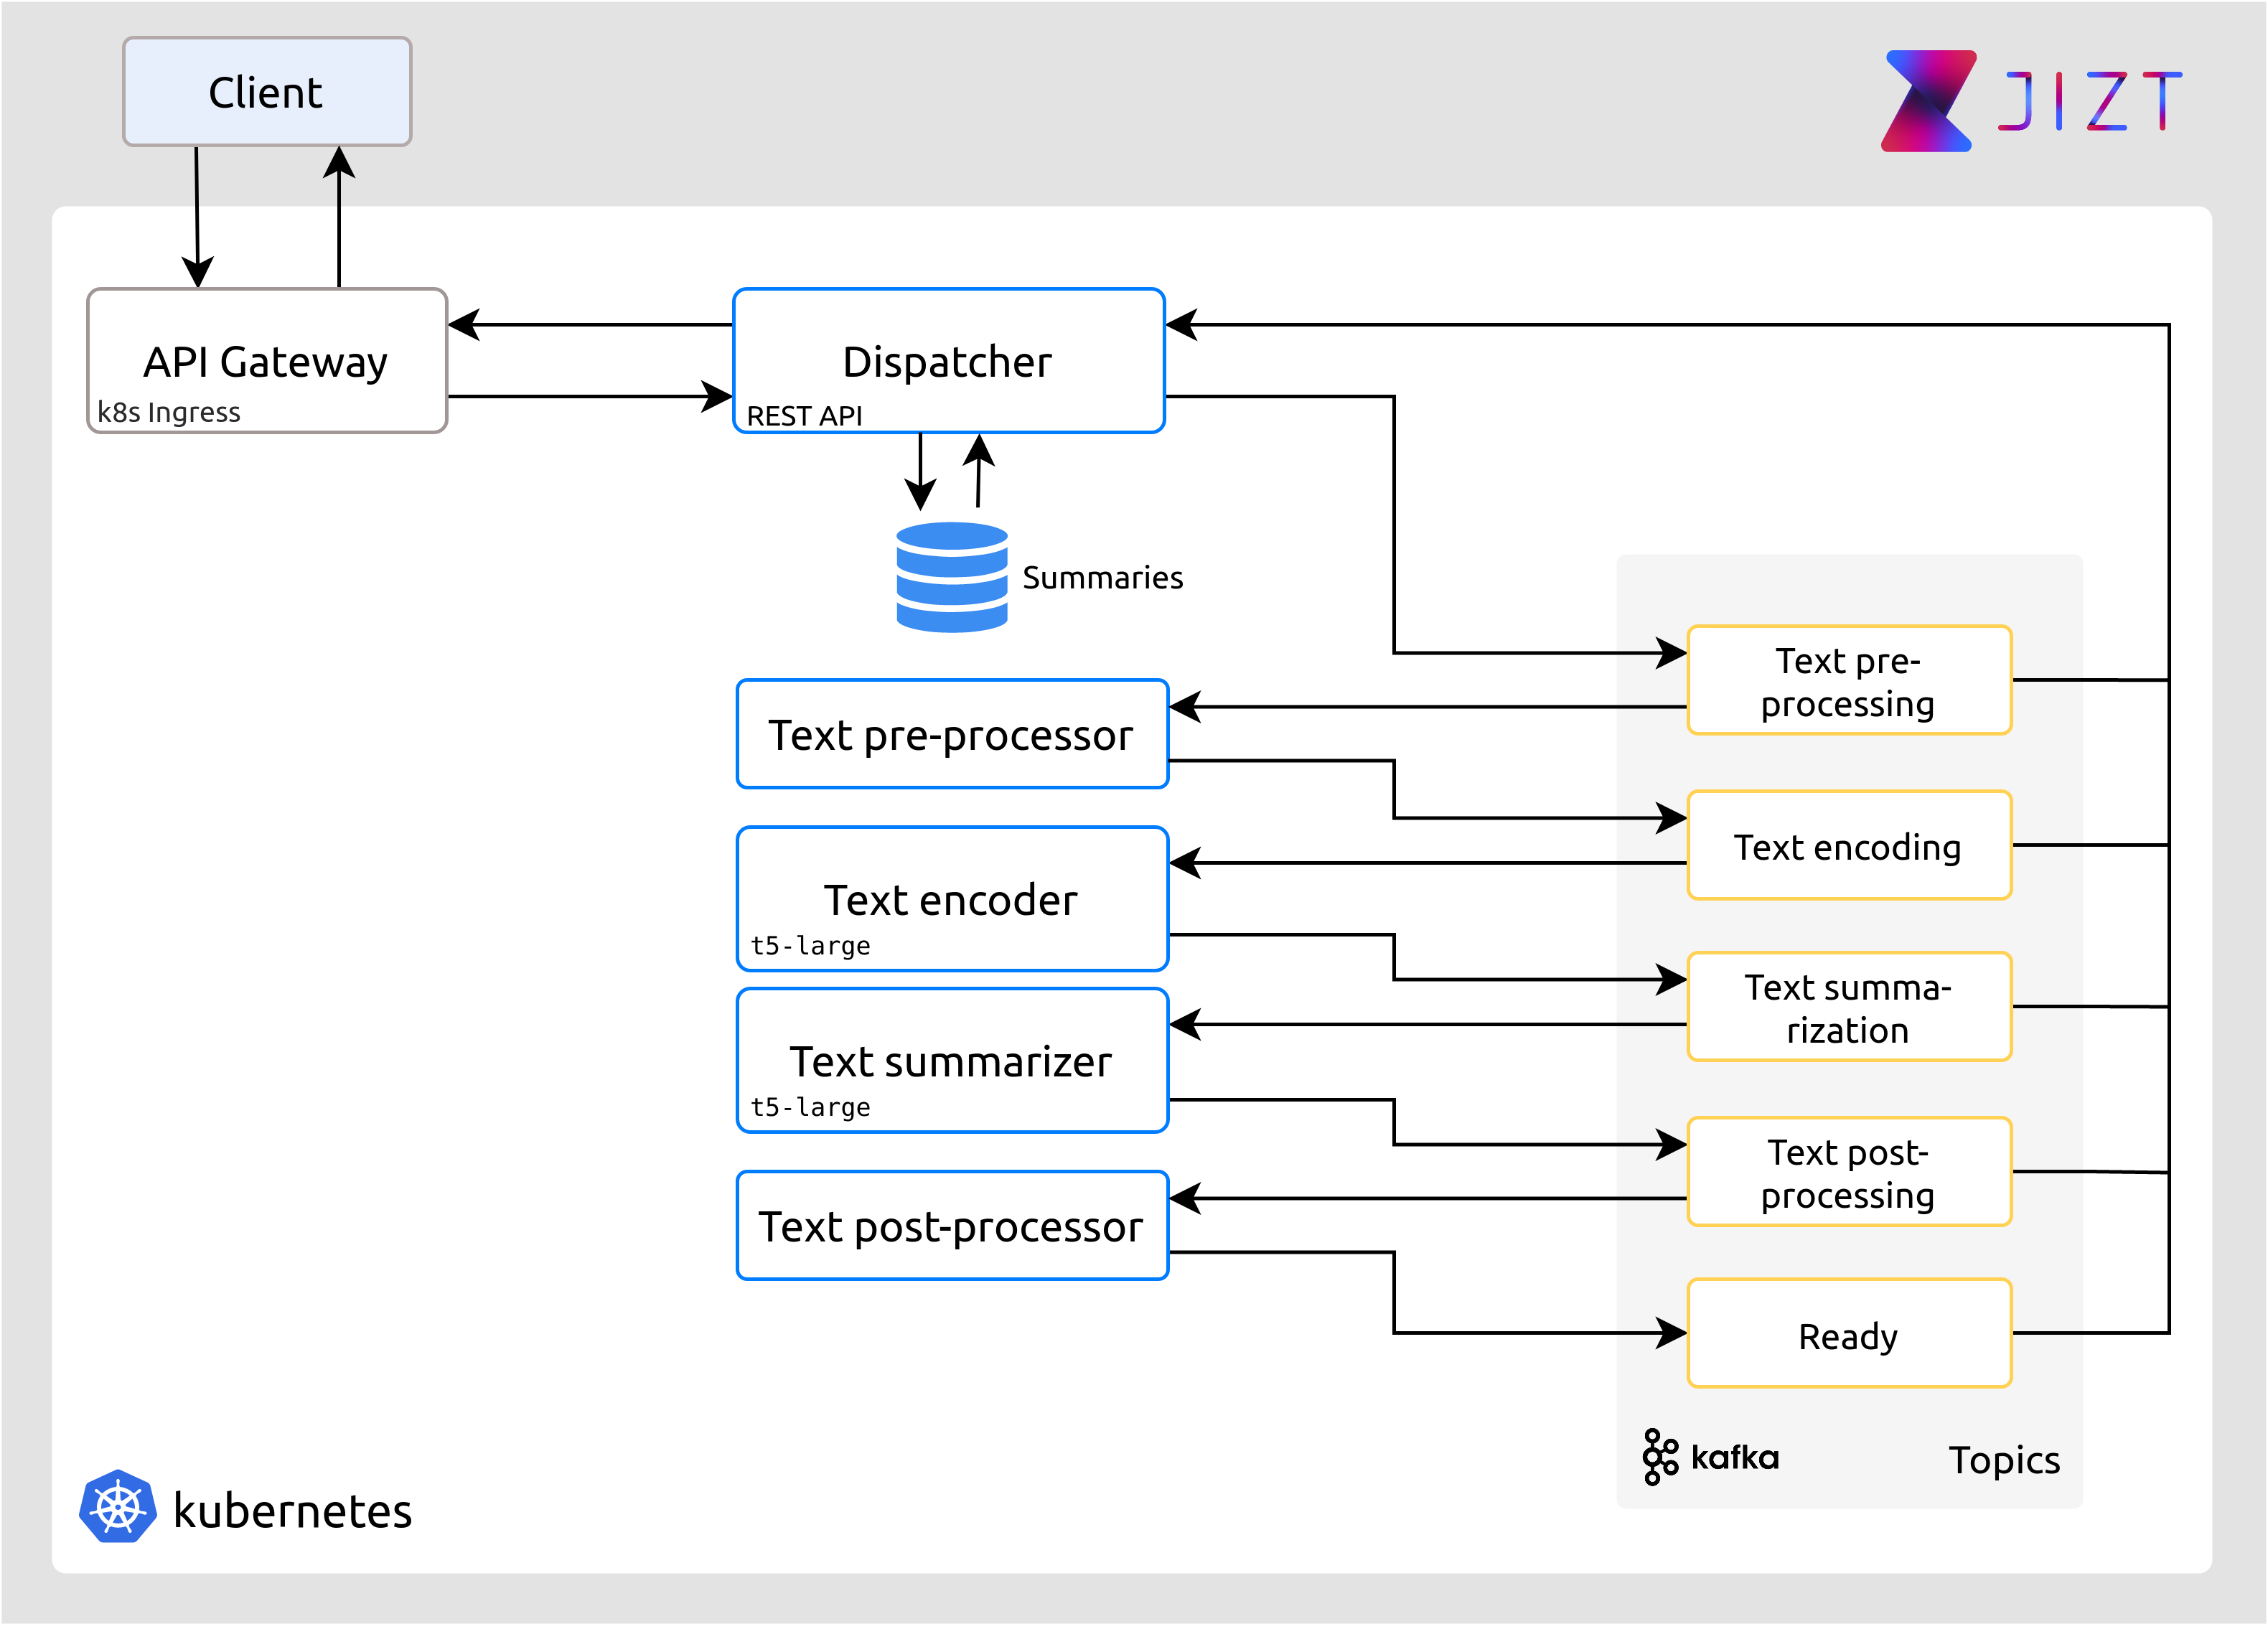
\includegraphics[width=\textwidth]{overview-arch}
	\vspace{-0.5cm}
	\caption{Diseño final de la arquitectura del \emph{backend}.}
	\label{fig:final-arch-backend}
\end{figure}

\begin{figure}[h!]
	\centering
	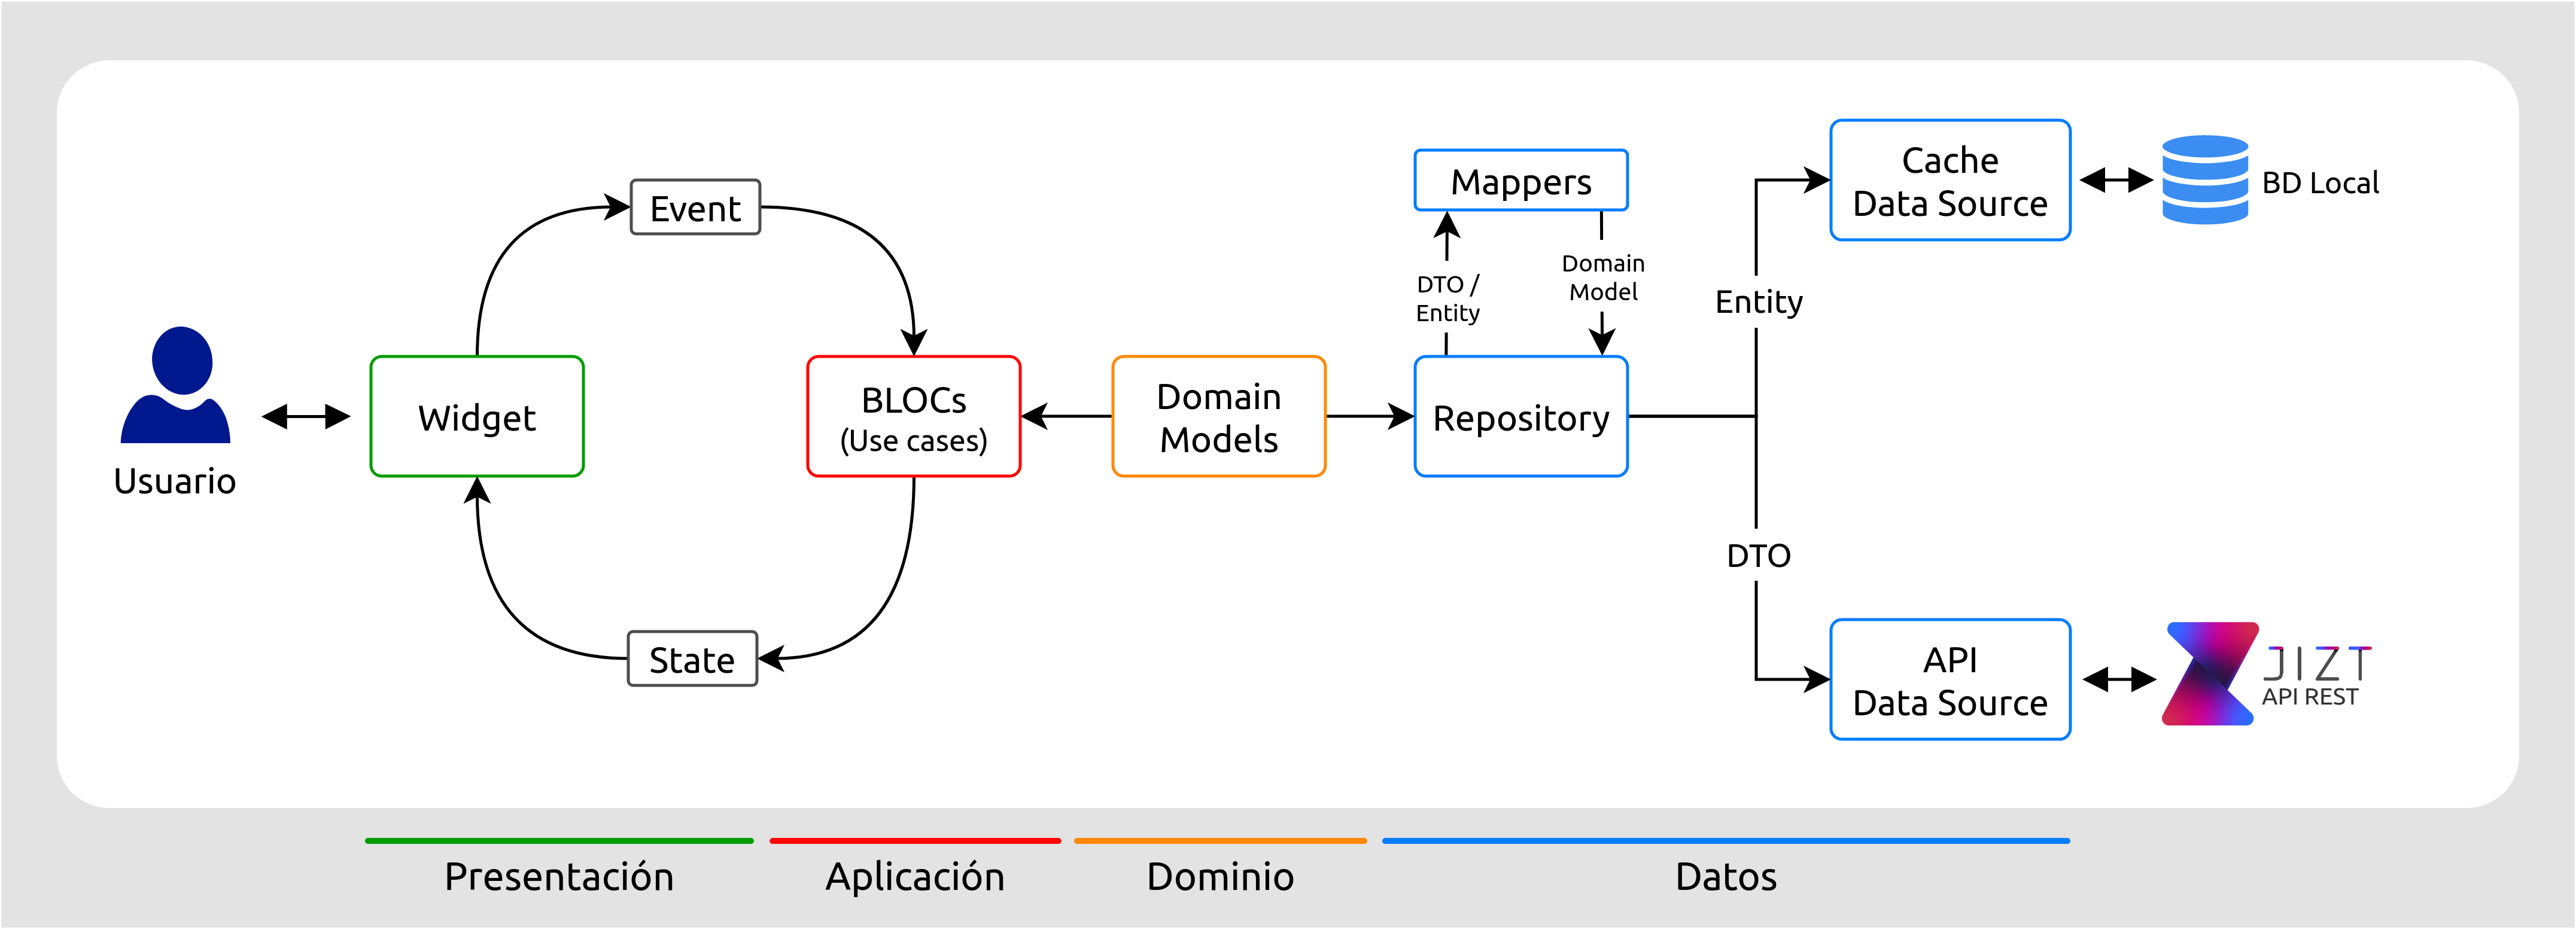
\includegraphics[width=\textwidth]{jizt-app-arch}
	\vspace{-0.5cm}
	\caption{Diseño final de la arquitectura de la aplicación.}
	\label{fig:final-arch-app}
\end{figure}

\newpage

\section{Diseño de interfaces}

\subsubsection{Diseño del logo}

Una de las intenciones detrás de este proyecto siempre ha sido tratar de crear una cierta imagen corporativa y de producto. Como consecuencia, el diseño de nuestra carta de presentación, es decir, nuestro logo, ocupó un papel central en las primeras iteraciones del proyecto.

En la búsqueda creativa de un logo atractivo, moderno y memorable, se experimentó con numerosos posibles diseños en papel.

\begin{figure}[h!]
	\centering
	\includegraphics[width=\textwidth]{logo-drafts}
	\vspace{-0.5cm}
	\caption{Ideas, ideas, y más ideas. Pero solo unas pocas buenas.}
\end{figure}

Finalmente, dimos con un diseño que parecía tener potencial. Cogimos nuestro ordenador, y nos sumergimos en Adobe Illustrator, un editor de gráficos vectoriales muy popular. Por experiencia previa en diseño gráfico (autodidacta), sabemos que, teniendo una buena idea de partida, equivale a tener una gran parte del trabajo hecho.

Así pues, el logo final, nuestra carta de presentación, acabó luciendo como se muestra en la \autoref{fig:jizt-logo}. En nuestra opinión, cumple con los requisitos esperados.

\newpage

\begin{figure}[h!]
	\centering
	
\includegraphics[width=0.8\textwidth]{jizt-logo}
	\caption{JIZT - Generación de resúmenes mediante IA.}
	\label{fig:jizt-logo}
\end{figure}

\vspace{0.3cm}

\begin{figure}[H]
	\centering
	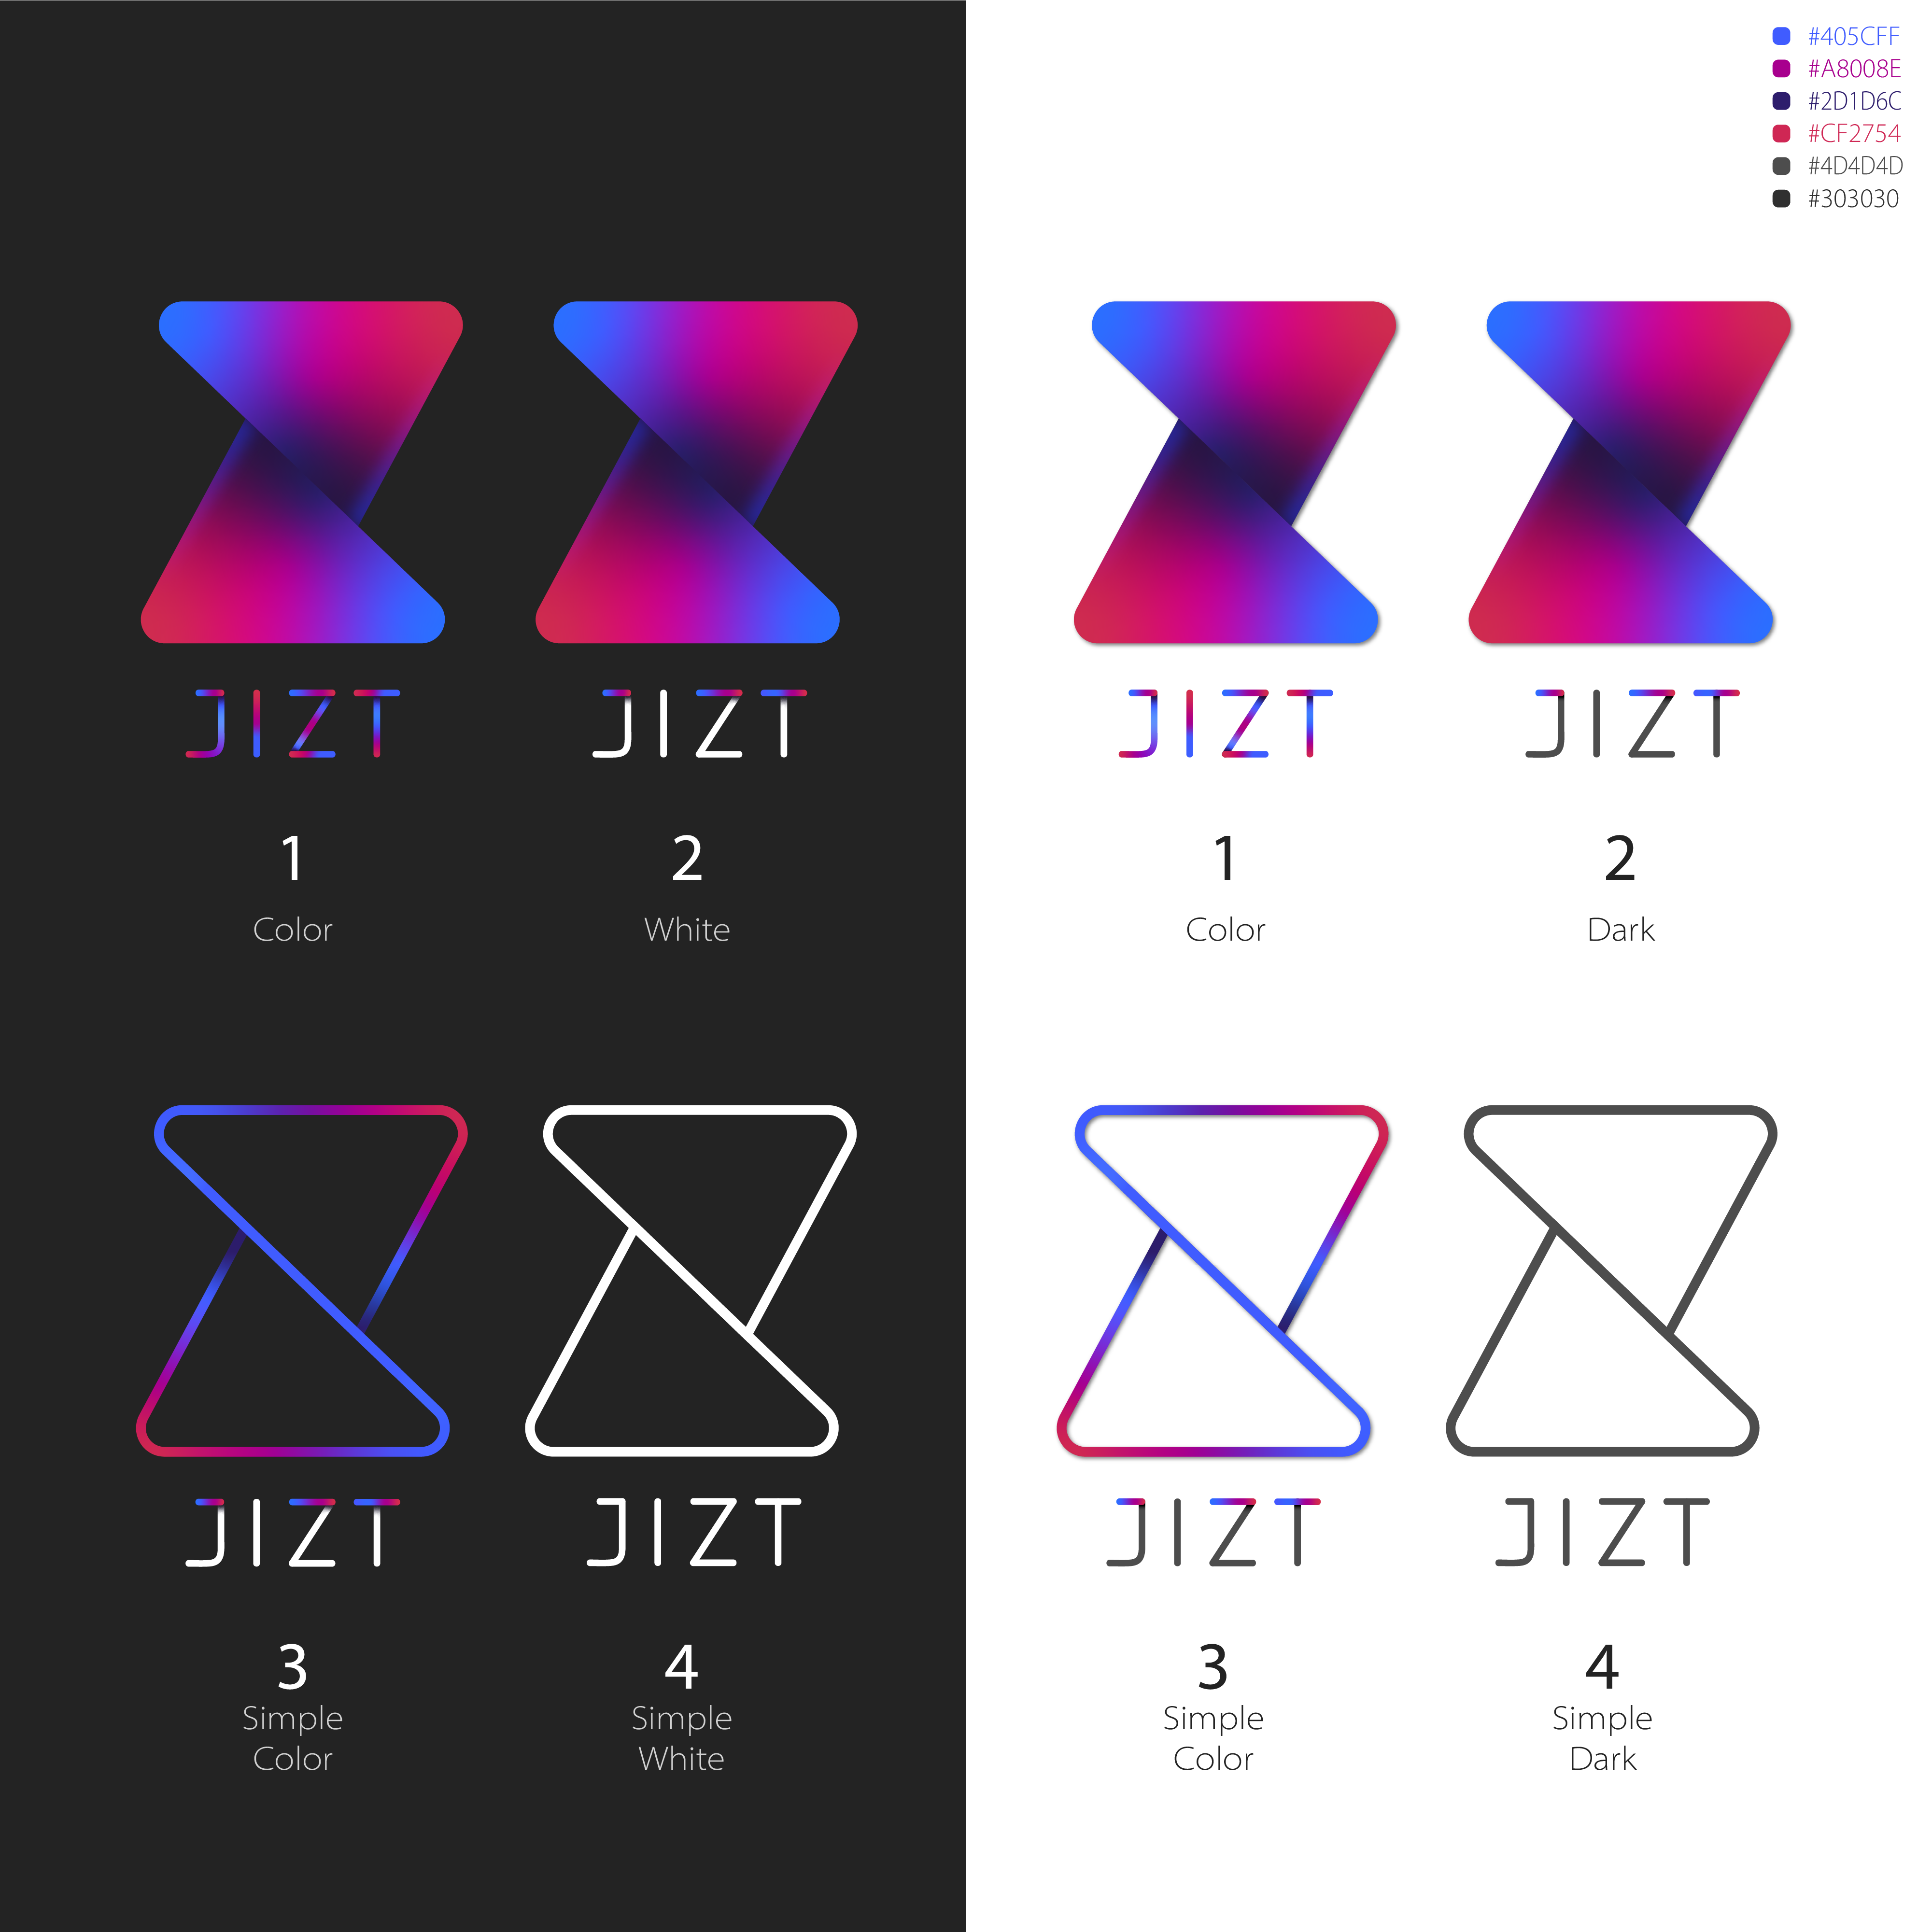
\includegraphics[width=0.91\textwidth]{jizt-logo-variations}
	\caption{Variaciones sobre el logo de JIZT.}
\end{figure}

\newpage

\subsubsection{Diseño de la interfaz gráfica de la aplicación}

Para el diseño de la interfaz gráfica de usuario de la aplicación, trabajamos directamente sobre el ordenador, esta vez con el programa Inkscape, también editor de gráficos vectoriales, pero en este caso \emph{open-source} y gratuito.

Se llevaron a cabo diferentes iteraciones hasta dar con un diseño que nos acabó pareciendo adecuado.

\bigskip

\begin{figure}[h!]
	\centering
	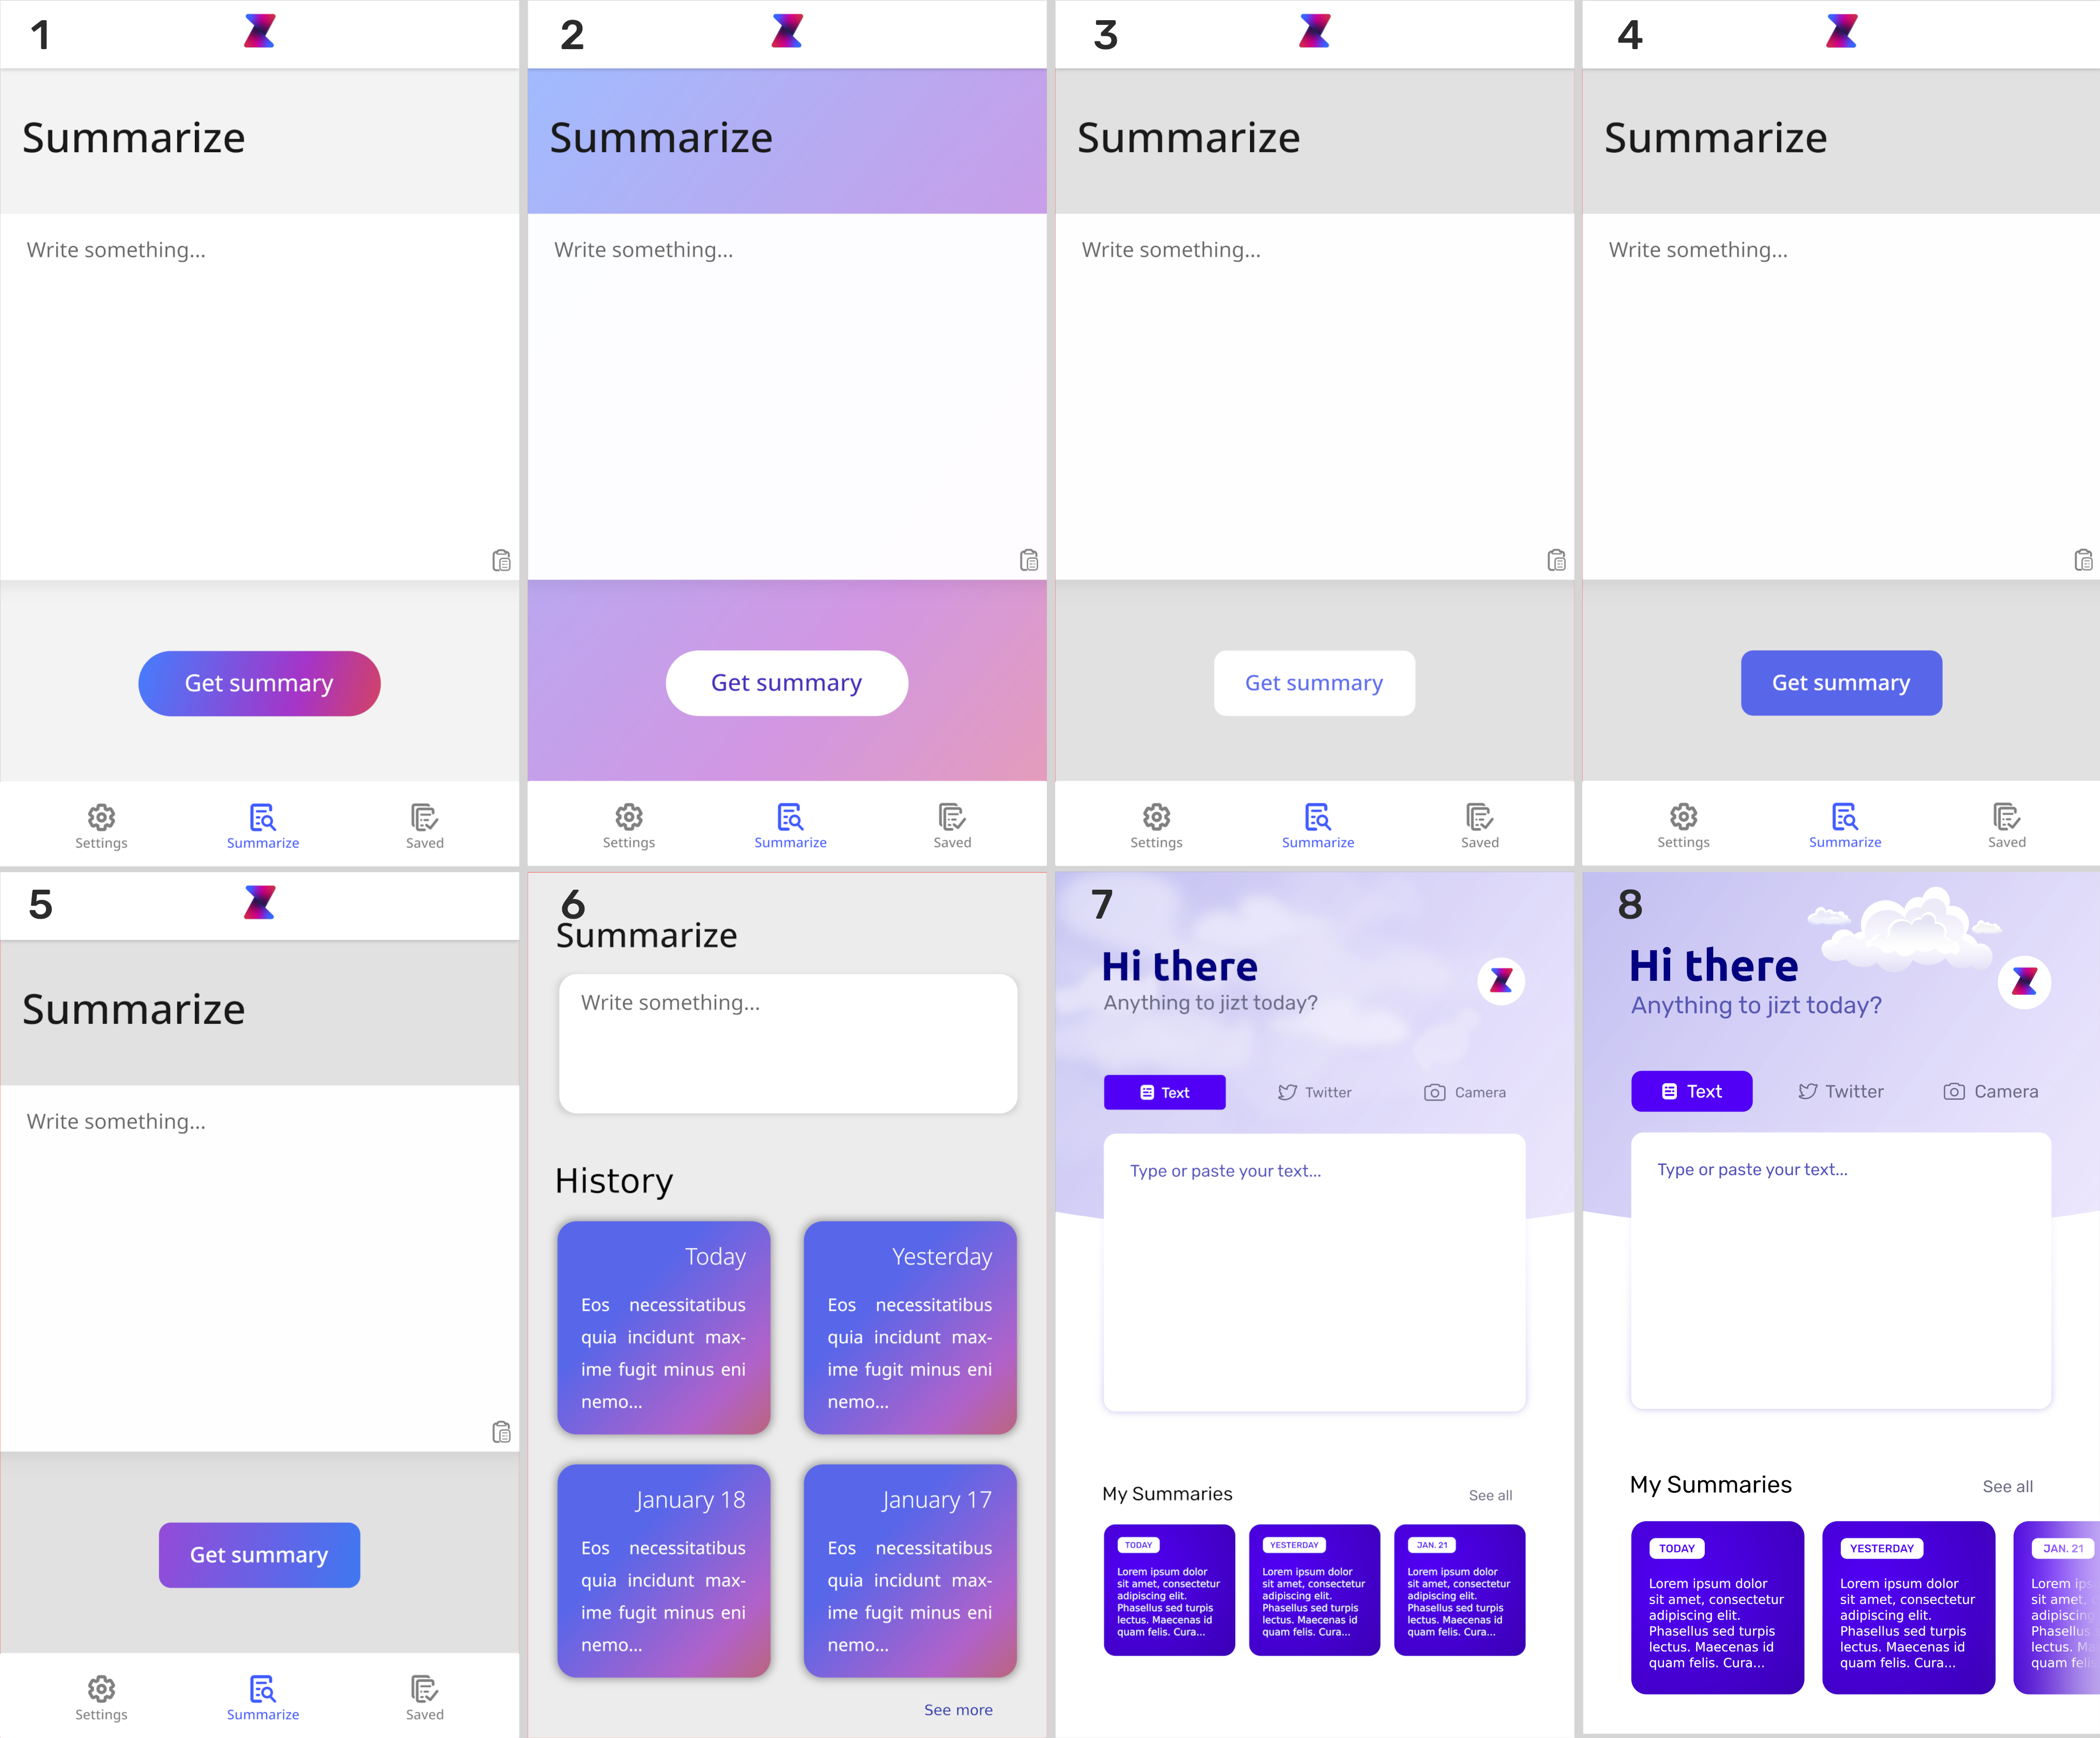
\includegraphics[width=\textwidth]{ui-design}
	\vspace{-0.5cm}
	\caption{Iteraciones sobre la pantalla principal.}
\end{figure}

Siguiendo el estilo de la pantalla principal, se diseñaron el resto de pantallas, las cuales se muestran en la \autoref{fig:app-screens}.

\newpage

\vspace*{1cm}
\begin{figure}[h!]
	\centering
	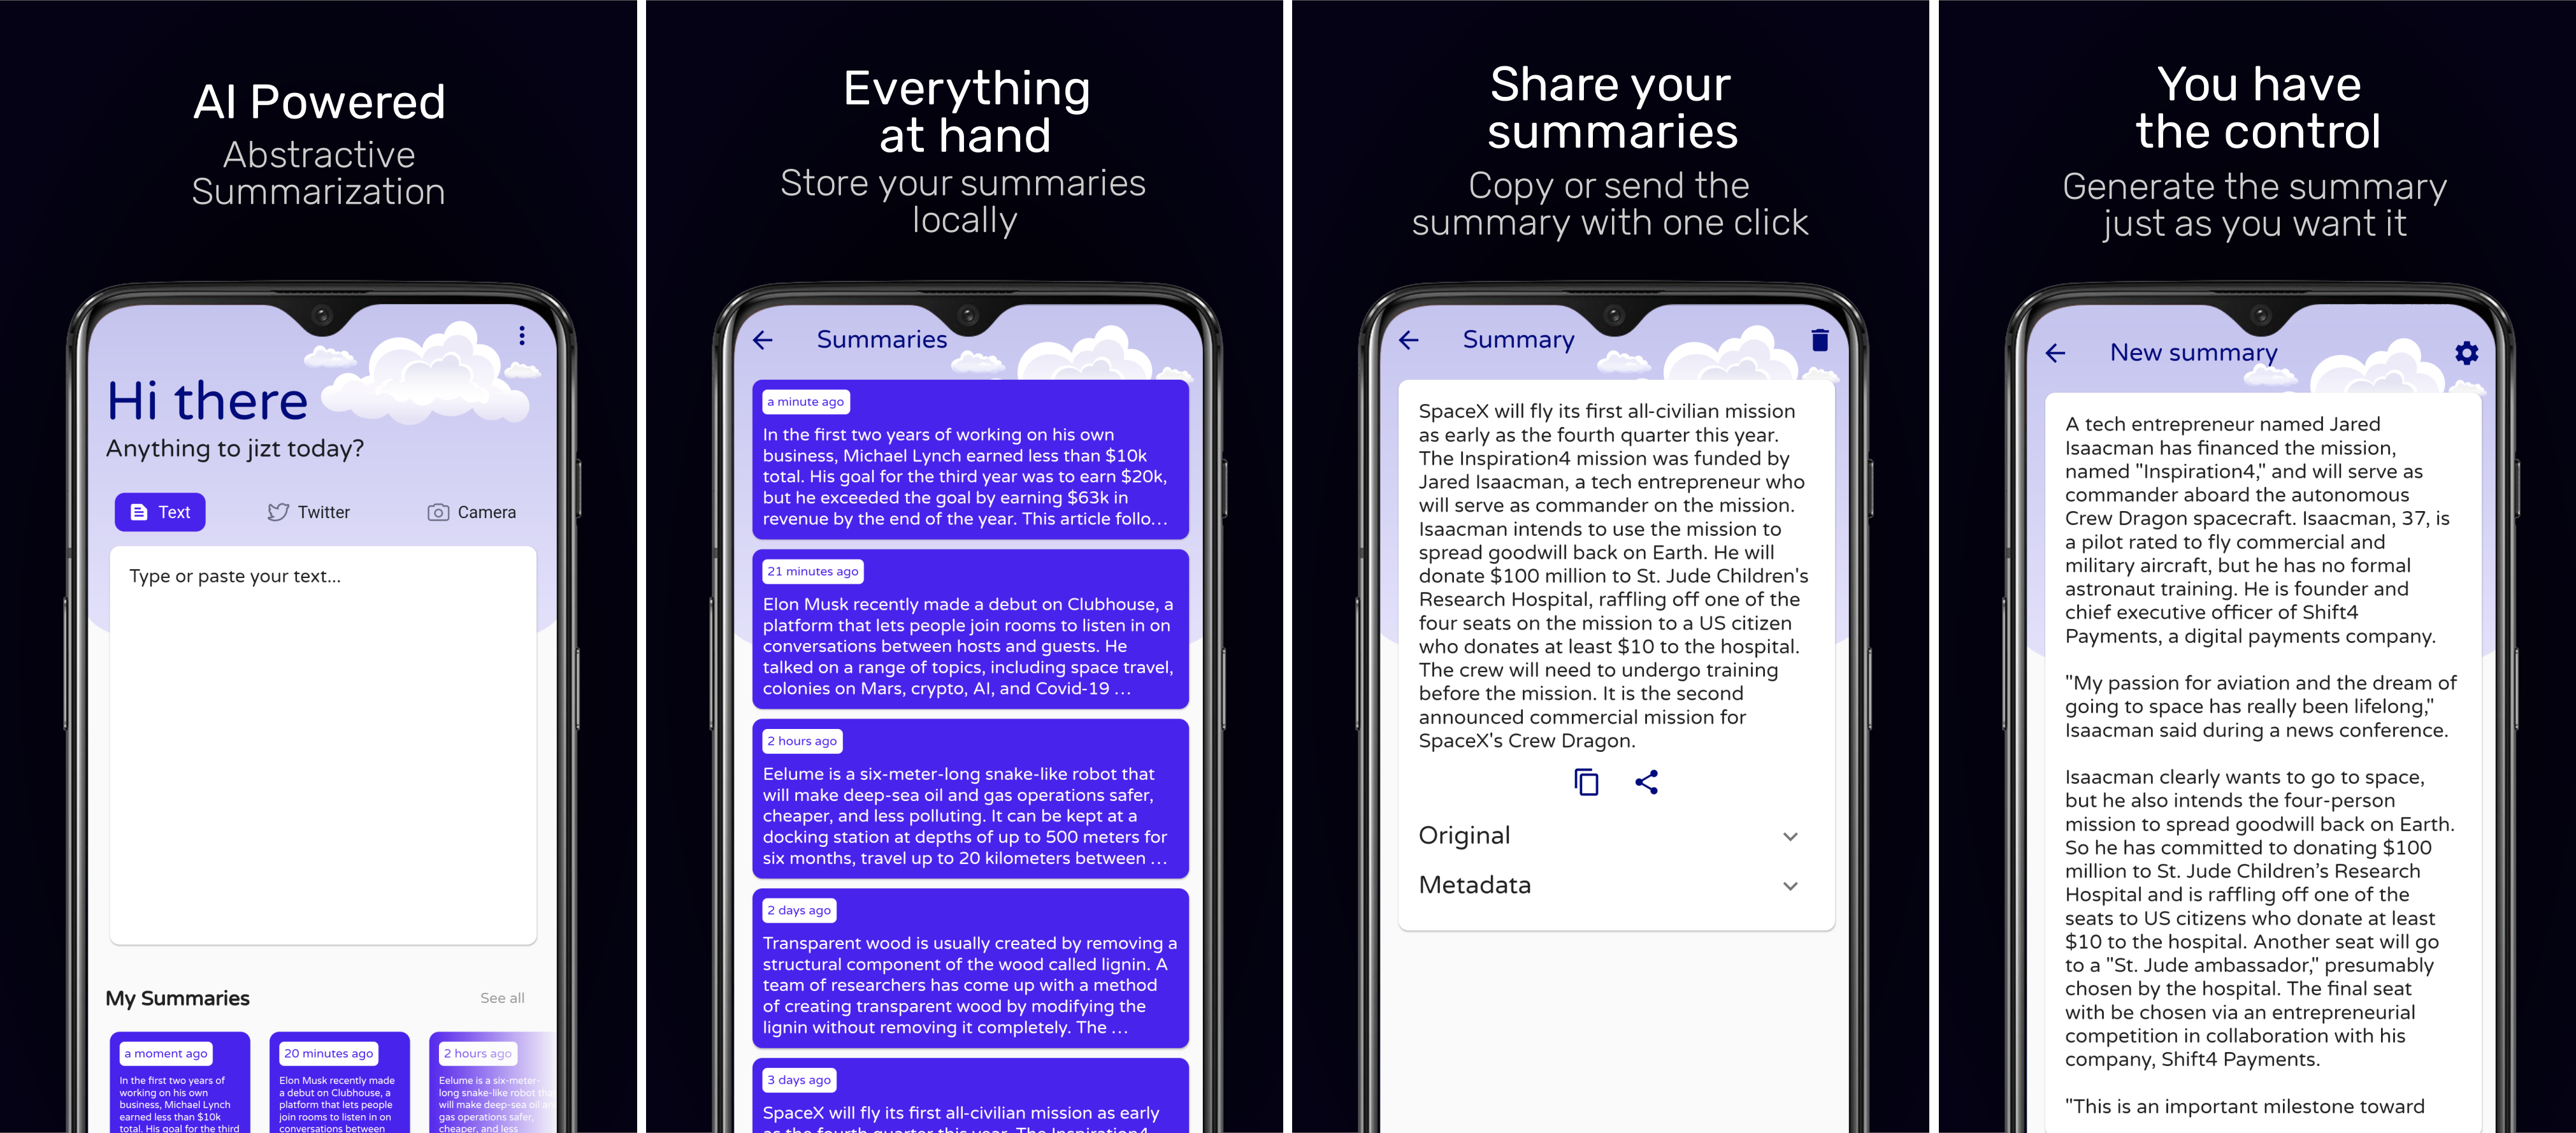
\includegraphics[width=\textwidth]{app-screens}
	\vspace{-0.5cm}
	\caption{Capturas de pantalla de la aplicación para su publicación en Play Store.}
    \label{fig:app-screens}
\end{figure}

\apendice{Documentación técnica de programación}

\section{Introducción}

\section{Estructura de directorios}

\section{Manual del programador}

\section{Compilación, instalación y ejecución del proyecto}

\section{Pruebas del sistema}

\apendice{Documentación de usuario} \label{apendice:usuario}

\section{Introducción}

En esta sección se recogen los requisitos que requiere nuestra aplicación, así como los detalles para la instalación y uso de la misma por el usuario final\footnote{\, Por ahora, no se incluyen los detalles referentes a la versión de escritorio, dado que el soporte de Flutter para estas plataformas está aún en fase \emph{alfa} \cite{flutter-desktop}.}.

\section{Requisitos de usuarios}

Para la versión \textbf{Android}, se deben cumplir los siguientes requisitos:

\vspace{-0.3cm}
\begin{itemize} [\textbullet]
	\item Mínimo 18 MB de espacio de almacenamiento libre. El paquete de instalación tiene un tamaño de 6,3 MB, y una vez instalada ocupa 16,36 MB. No obstante, ese tamaño aumentará ligeramente según se vayan almacenando resúmenes.
	
	\item Versión de Android igual o superior a la 4.1 (\emph{JellyBean} - API 16).
\end{itemize}

En el caso de \textbf{iOS}:

\vspace{-0.3cm}
\begin{itemize} [\textbullet]
	\item Mínimo 20 MB de espacio de almacenamiento libre. En este caso, el peso del paquete es de 6,9 MB, y una vez instalada ocupa 17,2 MB.
	
	\item Versión de iOS 8 o superior.
\end{itemize}

\newpage

Y en el caso de la versión \emph{\textbf{web}}:

\begin{itemize} [\textbullet]
	\item Los navegadores \emph{web} soportados son Google Chrome\footnote{Hemos probado la \emph{app} en navegadores basados en Chromium, como Brave, y también parecen funcionar.}, Mozilla Firefox, Safari o Edge.
\end{itemize}

En todos los casos se requiere conexión a Internet para generar nuevos resúmenes (los resúmenes ya generados se pueden consultar \emph{offline}). La \emph{app} de JIZT no requiere de permisos adicionales en ninguna de las plataformas.

La aplicación solo está disponible por el momento en inglés, dado que este es el único lenguaje soportado actualmente por el servicio de generación de resúmenes.

\vspace{2cm}

\section{Instalación}

En esta sección detallamos el proceso de instalación en las diferentes plataformas.

\subsection{Android}

\subsubsection{Instalación recomendada}

Se recomienda que el usuario instale la aplicación desde Google Play.

Para ello, simplemente basta con buscar la aplicación <<JIZT AI Summarization>> y pulsar en <<Instalar>>.

\newpage

\begin{figure}[H]
	\centering
	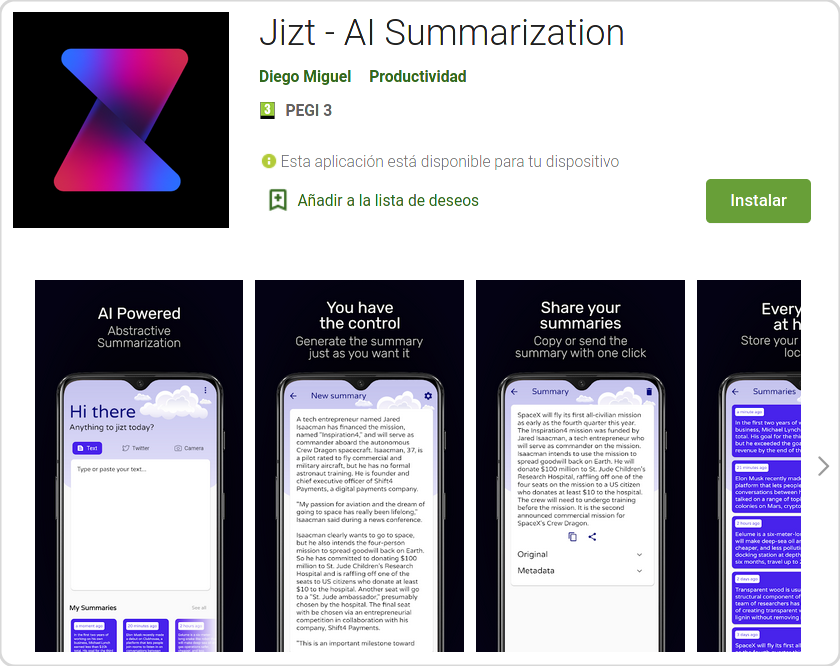
\includegraphics[width=0.8\textwidth]{jizt-google-play}
	\caption{Instalar JIZT desde Google Play.}
\end{figure}

\subsection{iOS}

Por el momento, la aplicación no ha sido publicada en la App Store, e iOS no proporciona ninguna manera oficial para la instalación de aplicaciones desde fichero\footnote{\, Como aclaración al margen de Manual de Usuario, la aplicación no ha sido publicada en la App Store por su elevado precio (99\$ al año por la cuenta de desarrollador, frente a los 25\$ de por vida, en el caso de Play Store).}.

Por tanto, se recomienda a los usuarios que accedan desde su navegador móvil a la versión \emph{web} de JIZT (ver siguiente sección).

\subsection{\emph{Web}}

Se puede acceder a la aplicación directamente a través de \href{https://app.jizt.it}{app.jizt.it}, sin ser necesario realizar ninguna instalación.

\newpage

\section{Manual del usuario}

Una vez instalada la aplicación, el usuario está en disposición de comenzar a utilizarla. El funcionamiento en interfaz de la aplicación en las diferentes plataformas es homogéneo, por lo que todo lo explicado a continuación es válido para cualquiera de ellas.

\subsection{Generar un nuevo resumen} \label{subsection:nuevo-resumen}

La generación de resúmenes se trata de una de las funciones principales de la aplicación.

Los pasos que debemos seguir para generar un nuevo resumen son los siguientes:

\begin{enumerate}
	\item En la pantalla de inicio, pulsar sobre el campo de texto central, el cual contiene escrito <<\emph{Type or paste your text}>> (en español, <<Escribe o pega tu texto>>).
	
	\item Escribir el texto o pulsar en el icono de la esquina superior derecha, el sirve para pegar el texto desde el portapapeles.
	
	\item Pulsar en <<\emph{Summarize}>> (<<resumir>>).
	
	\item Se mostrará una barra que simboliza que el resumen está siendo generado.
	
	\item Una vez completado el resumen, se mostrará una nueva pantalla con el resumen.
\end{enumerate}

Se puede visualizar un vídeo que recoge el proceso en \href{https://github.com/dmlls/jizt/blob/main/docs/video-tutorials/1-generar-nuevo-resumen.mp4}{https://github.com/\newline dmlls/jizt/blob/main/docs/video-tutorials/1-generar-nuevo-resumen.mp4}.

\subsection{Ajustar la longitud del resumen a generar}

JIZT nos permite establecer la longitud deseada del resumen generado. Esta longitud se establece como un porcentaje de la longitud del texto original.

Para ajustar la longitud del resumen que vamos a generar, debemos seguir los dos primeros pasos indicados en la sección <<\hyperref[subsection:nuevo-resumen]{Generar un nuevo resumen}>>.

Una vez en la pantalla de nuevo resumen, podemos ajustar el \emph{slider} que aparece en la parte inferior de la pantalla, estableciendo la longitud mínima y máxima de nuestro resumen.

Se puede visualizar un vídeo que recoge el proceso en \href{https://github.com/dmlls/jizt/blob/main/docs/video-tutorials/2-ajustar-longitud.mp4}{https://github.com/\newline dmlls/jizt/blob/main/docs/video-tutorials/2-ajustar-longitud.mp4}.

\subsection{Ver todos los resúmenes generados}

La aplicación muestra en la pantalla principal una vista previa de los últimos resúmenes generados en forma de lista deslizable. Pulsando sobre cualquiera de ellos, se accede a los detalles del mismo.

Si se quieren ver todos los resúmenes, se puede pulsar en <<\emph{See all}>> (<<ver todos>>). Se mostrará una nueva pantalla en la que aparece una lista con todos los resúmenes, ordenados temporalmente de más recientes a más antiguos. Se puede pulsar sobre cualquiera de ellos para obtener más detalles.

Se puede visualizar un vídeo que recoge el proceso en \href{https://github.com/dmlls/jizt/blob/main/docs/video-tutorials/3-ver-todos-resúmenes.mp4}{https://github.com/\newline dmlls/jizt/blob/main/docs/video-tutorials/3-ver-todos-resúmenes.mp4}.

\subsection{Borrar un resumen} \label{subsection:borrar}

Para borrar un resumen, se puede pulsar en el símbolo que aparece en la esquina superior derecha en la pantalla de <<\emph{Summary}>> (resumen).

Se puede acceder a esta pantalla de tres formas diferentes:

\begin{enumerate}
	\item Tras generar un resumen, se muestra dicha pantalla por defecto.
	
	\item Haciendo \emph{click} en cualquiera de los resúmenes que aparecen en la parte inferior de la pantalla principal.
	
	\item Pulsando en <<\emph{See all}>> (<<ver todos>>) y haciendo \emph{click} en cualquiera de los resúmenes.
\end{enumerate}

Se puede visualizar un vídeo que recoge el proceso en \href{https://github.com/dmlls/jizt/blob/main/docs/video-tutorials/4-borrar-resumen.mp4}{https://github.com/\newline dmlls/jizt/blob/main/docs/video-tutorials/4-borrar-resumen.mp4}.

\subsection{Copiar un resumen}

Para copiar un resumen, se debe estar en la pantalla de <<\emph{Summary}>> (resumen). Para acceder a esta pantalla, seguir cualquiera de las alternativas listadas en la sección ``\hyperref[subsection:borrar]{Borrar un resumen}''.

Una vez en esta pantalla, se debe pulsar en el siguiente icono:

Tras pulsar dicho icono, el texto se habrá copiado al portapapeles de nuestro dispositivo.

Se puede visualizar un vídeo que recoge el proceso en \href{https://github.com/dmlls/jizt/blob/main/docs/video-tutorials/5-copiar-resumen.mp4}{https://github.com/\newline dmlls/jizt/blob/main/docs/video-tutorials/5-copiar-resumen.mp4}.

\subsection{Compartir un resumen}

Para copiar un resumen, se debe estar en la pantalla de <<\emph{Summary}>> (resumen). Para acceder a esta pantalla, seguir cualquiera de las alternativas listadas en la sección ``\hyperref[subsection:borrar]{Borrar un resumen}''.

Una vez en esta pantalla, se debe pulsar en el siguiente icono:

A continuación, se mostrará una lista de aplicaciones a través de las cuales se puede compartir el resumen.

Se puede visualizar un vídeo que recoge el proceso en \href{https://github.com/dmlls/jizt/blob/main/docs/video-tutorials/6-compartir-resumen.mp4}{https://github.com/\newline dmlls/jizt/blob/main/docs/video-tutorials/6-compartir-resumen.mp4}.

\subsection{Ver el texto a partir del cual se generó un resumen}

Para ver el texto original de un resumen, se debe estar en la pantalla de <<\emph{Summary}>> (resumen). Para acceder a esta pantalla, seguir cualquiera de las alternativas listadas en la sección <<\hyperref[subsection:borrar]{Borrar un resumen}>>.

Una vez en dicha pantalla, se debe pulsar sobre <<\emph{Original}>>.

Se puede visualizar un vídeo que recoge el proceso en \href{https://github.com/dmlls/jizt/blob/main/docs/video-tutorials/7-ver-original.mp4}{https://github.com/\newline dmlls/jizt/blob/main/docs/video-tutorials/7-ver-original.mp4}.

\subsection{Obtener más información acerca de un resumen}

Para obtener más información de un resumen, se debe estar en la pantalla de <<\emph{Summary}>> (resumen). Para acceder a esta pantalla, seguir cualquiera de las alternativas listadas en la sección <<\hyperref[subsection:borrar]{Borrar un resumen}>>.

Una vez en dicha pantalla, se debe pulsar sobre <<\emph{More info}>> (<<Más información>>).

Se puede visualizar un vídeo que recoge el proceso en \href{https://github.com/dmlls/jizt/blob/main/docs/video-tutorials/8-m\%C3\%A1s-info.mp4}{https://github.com/\newline dmlls/ jizt/blob/main/docs/video-tutorials/8-m\%C3\%A1s-info.mp4}.

\subsection{Generar un resumen a partir de un documento}

Por el momento, esta opción no está disponible. No obstante, pronto será implementada.

\subsection{Generar un resumen a partir de una imagen}

Por el momento, esta opción no está disponible. No obstante, pronto será implementada.


\printbibliography[title={Bibliografía}]

\end{document}
